\documentclass{article}

\usepackage{amsmath, amsthm, amssymb, amsfonts, physics}
\usepackage{thmtools}
\usepackage{graphicx}
\usepackage{setspace}
\usepackage{geometry}
\usepackage{float}
\usepackage[hidelinks]{hyperref}
\usepackage[utf8]{inputenc}
\usepackage[english]{babel}
\usepackage{framed}
\usepackage[dvipsnames]{xcolor}
\usepackage{tcolorbox}
\usepackage{ctex}
\usepackage{tikz-cd}
\usepackage{mathtools}
\usepackage{tabularx, tabulary}

\colorlet{LightGray}{White!90!Periwinkle}
\colorlet{LightOrange}{Orange!15}
\colorlet{LightGreen}{Green!15}
\colorlet{LightBlue}{Blue!15}

\newcommand{\HRule}[1]{\rule{\linewidth}{#1}}
\newcommand{\impt}[1]{\textcolor{blue}{\textbf{\textit{#1}}}}
\newcommand{\uimpt}[1]{\underline{\textbf{\textit{#1}}}}
\newcommand{\R}{\mathbb{R}}
\newcommand{\Z}{\mathbb{Z}}
\newcommand{\N}{\mathbb{N}}
\newcommand{\C}{\mathbb{C}}
\newcommand{\F}{\mathbb{F}}
\newcommand{\id}{\mathbb{I}}
\newcommand{\imag}{\mathrm{i}}
\newcommand{\cplx}{\mathbf{z}}
\newcommand{\conj}[1]{#1^{*}}
\newcommand{\conjt}[1]{#1^{\dagger}}
\newcommand{\re}[1]{\text{Re}(#1)}
\newcommand{\im}[1]{\text{Im}(#1)}
\newcommand{\planck}{\hbar}
\newcommand{\hilbert}{\mathcal{H}}
\newcommand{\ketpsi}{\ket{\psi}}
\newcommand{\ketPsi}{\ket{\Psi}}
\newcommand{\ketphi}{\ket{\phi}}
\newcommand{\ketPhi}{\ket{\Phi}}
\newcommand{\brapsi}{\bra{\psi}}
\newcommand{\braPsi}{\bra{\Psi}}
\newcommand{\braphi}{\bra{\phi}}
\newcommand{\braPhi}{\bra{\Phi}}
\newcommand{\ketplus}{\ket{+}}
\newcommand{\ketminus}{\ket{-}}
\newcommand{\braplus}{\bra{+}}
\newcommand{\braminus}{\bra{-}}
\newcommand{\ketx}{\ket{x}}
\newcommand{\brax}{\bra{x}}
\newcommand{\Span}[1]{\text{span}\{#1\}}
\newcommand{\intR}{\int_{\R}}
\newcommand{\dx}{\dd x}
\newcommand{\Sum}[2]{\sum_{#1}^{#2}}
\newcommand{\Sumi}[1]{\sum_{#1}}
\newcommand{\Prod}[2]{\prod_{#1}^{#2}}
\newcommand{\hamiltonian}{\hat{H}}
\newcommand{\oppos}{\hat{X}}
\newcommand{\opmtm}{\hat{P}}
\newcommand{\opuni}{\mathcal{U}}
\newcommand{\annih}{\hat{a}}
\newcommand{\creat}{\hat{a}^{\dagger}}
\newcommand{\opnum}{\hat{n}}
\newcommand{\proj}[1]{\Pi_{#1}}
\newcommand{\Prob}[1]{\text{Pr}(#1)}
\newcommand{\urep}{\mathfrak{U}}

\declaretheoremstyle[name=Theorem,]{thmsty}
\declaretheorem[style=thmsty,numberwithin=section]{theorem}
\tcolorboxenvironment{theorem}{colback=LightGreen}

\declaretheoremstyle[name=Postulate,]{poststy}
\declaretheorem[style=poststy,numberwithin=section]{postulate}
\tcolorboxenvironment{postulate}{colback=Lavender!45}

\declaretheoremstyle[name=Lemma,]{lemsty}
\declaretheorem[style=lemsty,numberwithin=section]{lemma}
\tcolorboxenvironment{lemma}{colback=LightOrange}

\declaretheoremstyle[name=Definition,]{defnsty}
\declaretheorem[style=defnsty,numberwithin=section]{definition}
\tcolorboxenvironment{definition}{colback=LightBlue}

\setstretch{1.2}
\geometry{
    letterpaper,
    textheight=9in,
    textwidth=6.5in,
    top=1in,
    headheight=12pt,
    headsep=25pt,
    footskip=30pt
}

\begin{document}

\title{ \normalsize \textsc{}
		\\ [2.0cm]
		\HRule{1.5pt} \\
		\LARGE \textbf{\uppercase{ECON 301 - Intermediate Microeconomic Analysis}
		\HRule{2.0pt} \\ [0.6cm] \LARGE{进阶微观经济学分析} \vspace*{10\baselineskip}}
		}
\date{}
\author{\textbf{Author} \\ 
		Wenyou (Tobias) Tian \\
        田文友 \\
		University of British Columbia \\
        英属哥伦比亚大学 \\
		2024}

\maketitle
\newpage

\tableofcontents
\newpage
\section{Mathematical Tools and Notations - 数学工具及符号标记}
This first section is motivated by commonly-used symbolic notations and relevant mathematical tools required to perform analyses and calculations.

\subsection{Notations - 符号标记}
The most commonly used notations in this note include the following: \\
\begin{tabularx}{\textwidth}{p{1in}X}
    $\imag$ & different from ``$i$'', this represents the imaginary unit. Notice that $\frac{1}{\imag} = -\imag = \conj{\imag}$. \\
    $\abs{\cplx}$ & the norm of the complex number $\cplx$. \\
    $\re{\cplx}, \im{\cplx}$ & the real part and the imaginary part of complex number $\cplx$. \\
    $\conj{\cplx}$ & the complex conjugate of complex number $\cplx$. \\
    $\dagger$ & superscript symbol to denote the complex adjoint of a matrix. \\
    $\hilbert$ & a Hilbert space, a mathematical notation used to denote a \impt{quantum system}. \\
    $\ketpsi$ & usually represents a normalized vector in a given $\hilbert$, a mathematical notation used to denote a \impt{quantum state} in a quantum system. \\
    $\braket{\phi}{\psi}$ & mathematically, it represents the \textit{inner product} of $\ketphi$ and $\ketpsi$. \\
    $\dyad{\phi}{\psi}$ & mathematically, it represents the \textit{outer product} of $\ketphi$ and $\ketpsi$. \\
    $\ket{0}, \ket{1}$ & one set of basis vectors for a qubit, with $\ket{0} = \begin{pmatrix} 1 \\ 0 \end{pmatrix}$ and $\ket{1} = \begin{pmatrix} 0 \\ 1 \end{pmatrix}$. \\
    $\ketplus, \ketminus$ & another set of basis vectors for a qubit, with $\ketplus = \frac{1}{\sqrt{2}}\begin{pmatrix} 1 \\ 1 \end{pmatrix}$ and $\ketminus = \frac{1}{\sqrt{2}}\begin{pmatrix} 1 \\ -1 \end{pmatrix}$. \\
    $\delta(x)$ & \hyperref[subsec:dirac-delta]{\textcolor{cyan}{Dirac delta function}}. \\
    $\proj{x}$ & represents a projector onto one orthonormal basis $\ket{x}$, $\proj{x} = \dyad{x}{x}$. \\
    $\mathcal{O}$ & usually denotes an observable. \\
    $X, Y, Z$ & denote Pauli-X, Pauli-Y, Pauli-Z observables respectively. \\
    $\oppos, \opmtm$ & position observable and momentum observable. \\
    $H$ & denotes Hadamard operator, $H = \frac{1}{\sqrt{2}} \begin{pmatrix}
        1 & 1 \\
        1 & -1
    \end{pmatrix}$. \\
    $\hbar$ & reduced Planck's constant, $\approx 1.05 \times 10^{-34} \text{J} \cdot \text{s}$, $h = 2\pi\hbar$. It relates the frequency of wave/light with \impt{rotational velocity/angular frequency} $\omega$. We have $\omega = 2\pi f$, $hf = \hbar \omega$. It shows up when calculating the energy of a photon of wavelength $\lambda$: $f = \frac{c}{\lambda} \to \omega = \frac{2\pi c}{\lambda} \to \text{Experiments: } E_\lambda = \hbar \omega$. \\
    $\opuni$ & mostly denotes a unitary operator/evolution. \\
    $\hat{H}$ & denotes the Hamiltonian in a Schr\"odinger's equation. \\
    $[A, B]$ & commutator between matrices $A$ and $B$, if $[A, B] = 0$, the two matrices commutes, otherwise, one needs to add the difference. \\
    $\annih, \creat$ & the annihilation and creation operators. \\
    $\opnum$ & the number operator, equivalent to $\creat\annih$. \\
    $\tr(A)$ & trace of a square matrix $A$. \\
    $\mathfrak{U}$ & a unitary representation of a group on a Hilbert space. \\
    $\rho$ & the density operator.
\end{tabularx}
% ----------------------------------------------------------------
\subsection{Mathematical Tools - 数学工具}
\subsubsection{Complex Numbers - 复数}
A complex number $\cplx$ can be considered as a vector in a complex plane with coordinates $(a, b)$. Let the \impt{norm} of $\cplx$ be defined as \impt{$r = \sqrt{a^2 + b^2}$}, and the \impt{argument} (the angle between the vector and the positive real axis) of $\cplx$ be $\theta$. Then, the complex number $\cplx$ can be represented in a variety of ways:
\begin{definition}
    Given a complex number $\cplx$, its coordinates, and its argument, we have:
    $$\cplx = a + b\imag$$
    $$\cplx = re^{\imag \theta} = r(\cos \theta + \imag \sin \theta)$$
    We further denote the real part of this complex number $\re{\cplx} = a$, and the imaginary part $\im{\cplx} = b$.
\end{definition}
The second representation is well-defined due to \impt{Euler's formula}:
$$e^{\imag \theta} = \cos \theta + \imag \sin \theta$$
Furthermore, a useful byproduct of such a representation is the following:
\begin{definition}
    The complex conjugate of a complex number $\cplx$ is denoted as $\conj{\cplx}$, with properties:
    $$\conj{\cplx} = a - b\imag$$
    $$\conj{\cplx} = re^{-\imag \theta} = r(\cos \theta - \imag \sin \theta)$$
\end{definition}
It is trivial to notice that for a complex number $\cplx$ and its conjugate, their norms are equal,
$$\abs{\cplx} = \abs{\conj{\cplx}} = \sqrt{a^2 + b^2} = r, \abs{\cplx}^2 = \abs{\conj{\cplx}}^2 = \cplx \conj{\cplx}$$
and further gives us two useful properties:
$$\re{\cplx} = \frac{\cplx + \conj{\cplx}}{2}, \im{\cplx} = \frac{\cplx - \conj{\cplx}}{2\imag}$$
With the real part and the imaginary part of a complex number defined, we can also have:
\begin{align*}
    \re{\cplx} = 0 &\implies \cplx^2 = -\abs{\cplx}^2 \\
    \im{\cplx} = 0 &\implies \cplx^2 = \abs{\cplx}^2
\end{align*}
Further observations about the complex conjugate include the following:
\begin{quote}
    Let $\cplx_1, \cplx_2$ be two complex numbers, then: \\
    1. $\conj{(\cplx_1 + \cplx_2)} = \conj{\cplx_1} + \conj{\cplx_2}$ \\
    2. $\conj{(\cplx_1 \cplx_2)} = \conj{\cplx_1}\conj{\cplx_2}$ \\
    These two properties imply the \impt{linearity of conjugation}. \\
    3. $\im{\cplx} = 0 \implies \conj{\cplx} = -\cplx$. \\
    4. $r = 1 \implies \conj{\cplx} = \frac{1}{\cplx}$ (the complex number is \impt{unitary})
\end{quote}
\newpage
% ----------------------------------------------------------------
\subsubsection{Linear Algebra - 线性代数}
\begin{definition}
    Given a vector $\vec{\cplx}$ in a complex vector space, let
    $$\vec{\cplx} = \begin{pmatrix}
        \cplx_1 \\
        \cplx_2 \\
        \vdots \\
        \cplx_n
    \end{pmatrix}$$
    then, the \uimpt{conjugate (Hermitian) transpose} of $\vec{\cplx}$ is denoted as:
    $$\vec{\cplx}^{\dagger} = \begin{pmatrix}
        \conj{\cplx_1} & \conj{\cplx_2} & \dots & \conj{\cplx_n}
    \end{pmatrix}$$
    Similarly, given a matrix $A \in \C^{m \times n}$ over a complex vector space, with element on the $i$th row and $j$th column be $a_{ij}$, then the \uimpt{complex conjugate/adjoint} of $A$, denoted as $A^{\dagger} \in \C^{n \times m}$, has elements on the $j$th row and $i$th column be $a_{ji}' = \conj{a_{ij}}$. \\
    This yields:
    $$\vec{\cplx}^{\dagger} = \conj{(\vec{\cplx}^{\top})}$$
    $$A^{\dagger} = \conj{(A^{\top})}$$
\end{definition}
\label{subsec:hermitian}
\begin{definition}
    A linear operator $A: \hilbert \to \hilbert$ (or complex vector spaces in general) is \uimpt{self-adjoint (Hermitian)} if:
    $$A = A^{\dagger}$$
\end{definition}
\begin{theorem}
    \uimpt{Spectral decomposition for Hermitian operators}: \\
    Let $A$ be Hermitian, there exists an orthonormal basis $\{\ket{x}\}_x$ such that they are \uimpt{eigenvectors} of $A$, and \uimpt{all eigenvalues} $\lambda \in \R$.
\end{theorem}
This is to claim, there exists an orthonormal basis $\{\ket{x}\}_x$ such that
$$\forall x, A \ket{x} = \lambda_x \ket{x}, \lambda_x \in \R$$
where $\braket{x}{x'} = \delta_{xx'}$. We can then express this Hermitian operator as:
$$A = \Sumi{x} \lambda_x \dyad{x}{x} = \Sumi{x} \lambda_x \proj{x}$$
We say $\{\lambda_x\}$ \impt{form the spectrum}.
\label{subsec:unitary}
\begin{definition}
    A linear operator $\mathcal{U}: \hilbert \to \hilbert$ is a \uimpt{unitary operator} if we have
    $$\mathcal{U}\mathcal{U}^{\dagger} = \mathcal{U}^{\dagger}\mathcal{U} = \id$$
\end{definition}
We further denote the set of unitaries on $\hilbert$ by 
$$\opuni(\hilbert) = \{\opuni: \hilbert \to \hilbert \text{ is a linear operator} \mid \opuni\opuni^{\dagger} = \opuni^{\dagger}\opuni = \id\}$$
\begin{theorem}
    \uimpt{Spectral decomposition for Unitary operators}: \\
    Let $\opuni$ be unitary on $\hilbert$, there exists an orthonormal basis $\{\ket{k}\}_k$ of $\opuni$ such that all eigenvalues $\{\lambda_k\}_k$ have $\abs{\lambda_k} = 1$.
\end{theorem}
Hence, 
$$\opuni = \Sumi{k} \lambda_k \dyad{k}{k} = \Sumi{k}e^{\imag \alpha_k} \dyad{k}{k}$$
These properties indicate that unitary matrices are invertible; they preserve normalization and inner product. The proof of such preservation is as follows:
\begin{align*}
    (\opuni \ketphi, \opuni \ketpsi) &= \conjt{(\opuni \ketphi)} (\opuni \ketpsi) \\
    &= \mel{\phi}{\conjt{\opuni}\opuni}{\psi} \\
    &= \braket{\phi}{\psi}
\end{align*}
Generally, in a $d$-dimensional complex vector space, we can express $\opuni = VD\conjt{V}$ with $V$ being an orthonormal basis transformation and
$$D = \begin{pmatrix}
    e^{\imag \alpha_1} & \dots & 0 \\
    \vdots & \ddots & \vdots \\
    0 & \dots & e^{\imag \alpha_d}
\end{pmatrix}$$
\begin{definition}
    The \uimpt{tensor product} between two Hilbert spaces $\hilbert_A$ and $\hilbert_B$ is defined as:
    $$\hilbert_A \otimes \hilbert_B := \text{span}\{\ketpsi_A \otimes \ketphi_B \mid \ketpsi_A \in \hilbert_A, \ketphi_B \in \hilbert_B\}$$
\end{definition}
The tensor products have the following identifications:
\begin{quote}
    1. Multiplication with scalars: $\forall a \in \C, (a \ketpsi_A) \otimes \ketphi_B = \ketpsi_A \otimes (a \ketphi_B) = a(\ketpsi_A \otimes \ketphi_B)$. \\
    2. Distributive property: $(\ket{\psi_1}_A + \ket{\psi_2}_A) \otimes \ketphi_B = \ket{\psi_1}_A \otimes \ketphi_B + \ket{\psi_2}_A \otimes \ketphi_B$. \\
    3. How operators act: $(S_A \otimes T_B)(\ketpsi_A \otimes \ketphi_B) = (S_A \ketpsi_A) \otimes (T_B \ketphi_B)$. \\
    4. Inner products: $(\bra{\psi_1}_A \otimes \bra{\phi_1}_B)(\ket{\psi_2}_A \otimes \ket{\phi_2}_B) = \braket{\psi_1}{\psi_2}_A \braket{\phi_1}{\phi_2}_B$
\end{quote}
How do we make tensor products explicit? First, we start with single vectors. Consider two vectors:
$$\vec{x} = \begin{pmatrix}
    x_1 \\
    \vdots \\
    x_n
\end{pmatrix}, \vec{y} = \begin{pmatrix}
    y_1 \\
    \vdots \\
    y_m
\end{pmatrix}$$
Then, the tensor product of these two vectors is:
$$\vec{x} \otimes \vec{y} = \begin{pmatrix}
    x_1 \vec{y} \\
    \vdots \\
    x_n \vec{y}
\end{pmatrix} = \begin{pmatrix}
    x_1 y_1 \\
    \vdots \\
    x_1 y_m \\
    \vdots \\
    x_n y_1 \\
    \vdots \\
    x_n y_m
\end{pmatrix}$$
Then, this implies the tensor product for matrices. Consider two matrices:
$$A = \begin{pmatrix}
    a_{11} & \dots & a_{1n} \\
    \vdots & \ddots & \vdots \\
    a_{n1} & \dots & a_{nn}
\end{pmatrix} \in \C^{n \times n}, B = \begin{pmatrix}
    b_{11} & \dots & b_{1m} \\
    \vdots & \ddots & \vdots \\
    b_{m1} & \dots & b_{mm}
\end{pmatrix} \in \C^{m \times m}$$
Their tensor product will be:
$$A \otimes B = \begin{pmatrix}
    a_{11} B & \dots & a_{1n} B \\
    \vdots & \ddots & \vdots \\
    a_{n1} B & \dots & a_{nn} B
\end{pmatrix} \in \C^{mn \times mn}$$

\label{subsec:commutator}
\begin{definition}
    Given two matrices $A, B$, define their \uimpt{commutator} to be
    $$[A, B] = AB - BA$$
    If $[A,B] = 0$, we say $A$ and $B$ are \uimpt{commutative} or \uimpt{commutes with each other}. 
\end{definition}
\begin{lemma}
    Two diagonalizable operators commute if and only if there exists a common eigenbasis between the two operators.
\end{lemma}
The proof of this lemma is as follows: \\
We first show the backward deduction. We assume that $A, B$ share an eigenbasis. Hence, in this basis, we can diagonalize the two matrices with its eigenvalues:
$$A = \begin{pmatrix}
    a_1 &  & \\
    & a_2 & \\
    & & \ddots
\end{pmatrix}, B = \begin{pmatrix}
    b_1 &  & \\
    & b_2 & \\
    & & \ddots
\end{pmatrix}$$
Thus, we have
$$AB = BA = \begin{pmatrix}
    a_1b_1 &  & \\
    & a_2b_2 & \\
    & & \ddots
\end{pmatrix}$$
Then we show the forward deduction. We assume $AB=BA$ and $\ket{k}$ is an eigenvector of $A$, then
$$AB\ket{k} = BA\ket{k} = B(\alpha_k \ket{k}) = \alpha_k B\ket{k}$$
This means that $B\ket{k}$ is an eigenvector of $A$ with the same eigenvalue. With the loss of generality, the same holds for all eigenvectors of $A$ and vice versa for $B$. This means that $A$ and $B$ share the same eigenspace, meaning there exists a same eigenbasis.
\begin{theorem}
    We define the exponentiation of a matrix $A$ with base $e$ to be:
    $$e^A = \Sum{n = 0}{\infty} \frac{A^n}{n!}$$
\end{theorem}
\begin{definition}
    The \uimpt{trace} of a square matrix $A$ is the sum of elements on its main diagonal. It is also the \uimpt{sum of eigenvalues} of the matrix. We denote the trace of $A$ to be $\tr(A)$.
\end{definition}
We have the following theorems for the trace:
\begin{theorem}
    Linearity of trace:
    $$\tr(\alpha A + \beta B) = \alpha \tr(A) + \beta \tr(B)$$
\end{theorem}
\begin{theorem}
    Cyclic property of the trace:
    $$\tr(AB) = \tr(BA)$$
    This further yields:
    $$\tr([A,B]) = 0$$
\end{theorem}
\begin{theorem}
    The trace of a matrix $\tr(A)$ is \uimpt{independent} of the basis chosen to represent $A$.
\end{theorem}
A useful property of the trace is that:
$$\tr(A) = \Sum{k=1}{d} \ev{A}{\phi_k}$$
with orthonormal basis $\{\ket{\phi_k}\}_{k=1}^d$.
\begin{definition}
    A \uimpt{group} is defined to be a set with an \uimpt{associative operation}. Consider a set $G$ and an operation $\cdot$, we can form a group if given $a, b \in G$ and $a \cdot b \in G$, we further have
    \begin{quote}
        1. $(a \cdot b) \cdot c = a \cdot (b \cdot c)$. \\
        2. $\exists \id, a \cdot \id = a$ \\
        3. $\exists a^{-1}, a \cdot a^{-1} = \id$
    \end{quote}
\end{definition}

\newpage
% ----------------------------------------------------------------
\subsubsection{Analysis - 分析}
\label{subsec:dirac-delta}
\begin{definition}
    A \uimpt{Dirac delta function} $\delta(x)$ is defined as
    $$\intR \delta(x) f(x) \dx = f(0) \to \intR \delta(x-y)f(x) \dx = f(y)$$
    such that it has the property
    $$\delta(x) = \begin{cases}
        0 & x \ne 0 \\
        +\infty & x = 0
    \end{cases}$$
    $$\intR \delta(x) \dx = 1$$
\end{definition}
There are some other useful properties of the Dirac delta function, which are as follows:
$$\delta(ax) = \frac{1}{\abs{a}}\delta(x) \implies \delta(-x) = \delta(x)$$
$$\delta(x) = \frac{1}{2\pi} \intR e^{\imag px} \dd p = \frac{1}{2\pi\hbar} \intR \exp(\frac{\imag p x}{\hbar}) \dd p$$

\label{subsec:fourier}
\begin{definition}
    Let $f: \R \to \R$ be an integrable function. The \uimpt{Fourier transform} of $f$ is a function $F$ defined as:
    $$F(t) = \mathcal{F}[f] = \frac{1}{\sqrt{2\pi}} \intR f(x) \exp(-\imag t x) \dd x$$
    The inverse of the Fourier transform is another Fourier transform:
    $$f(x) = \mathcal{F}^{-1}[F] = \frac{1}{\sqrt{2\pi}} \intR F(t) \exp(\imag t x) \dd t$$
    An extra form of the Fourier transform is:
    $$f(x) = \frac{1}{\sqrt{2k\pi}} \intR F(t) \exp(\frac{\imag t x}{k}) \dd t$$
\end{definition}
\begin{theorem}
    The linearity of the transform indicates:
    $$\forall a, b \in \C, \mathcal{F}[af+bg] = a\mathcal{F}[f] + b\mathcal{F}[g]$$
\end{theorem}
\begin{theorem}
    The transform of derivatives indicates:
    $$\mathcal{F}[f'] = \frac{\imag p}{\hbar} \mathcal{F}[f]$$
\end{theorem}
\begin{theorem}
    The transform of the shift indicates that:
    $$\mathcal{F}[f(x-x_0)] = \exp(-\imag p x_0)\mathcal{F}[f]$$
\end{theorem}

\label{subsec:differential-eqn}
\begin{theorem}
    Consider a $2^{nd}$ degree ordinary differential equation of the form
    $$y'' + py' + y = 0$$
    We further consider its relating quadratic equation:
    $$\lambda^2 + p\lambda + q = 0$$
    where its solution is one of the following scenarios:
    \begin{quote}
        1. Two unequal real roots $a \ne b$. \\
        2. Two equal real roots $a = b$. \\
        3. Two complex roots $\alpha \pm \imag \beta$.
    \end{quote}
    The general solution to the ODE is the following in respective scenarios:
    \begin{quote}
        1. $y = c_1e^{ax} + c_2e^{bx}$. \\
        2. $y = c_1e^{ax} + c_2xe^{ax}$. \\
        3. $y = c_1e^{\alpha x}\cos(\beta x) + c_2e^{ax}\sin(\beta x) = c_1e^{(\alpha + \imag \beta)x} + c_2e^{(\alpha - \imag \beta)x}$
    \end{quote}
\end{theorem}

\newpage
\section{Postulates of Quantum Physics - 量子物理的“公理”}
\subsection{Postulate 1 - “公理”一}
Quantum physics/mechanics are usually taught as a subsequent course of undergraduate classical physics course. In this course, however, we directly develop from the postulates to describe physics quantum-mechanically. \par
This includes describing the physics of particles (e.g. electrons, photons, single atoms), many-body systems, superconducting systems, which are small systems, and even large systems like the solar system or the entire universe. We may also wish to describe different degrees of freedom -- vectorial degrees of freedom (e.g. continuous degrees of freedom like \impt{position} or \impt{momentum}, and discrete/countable degrees of freedom like \impt{spin}), and scalar degrees of freedom (e.g. mass, charge, phase etc.). \par
To simplify our analyses, we may choose to describe certain degrees of freedom in a quantum mechanical way, and others classically. For example:
\begin{quote}
    Consider an electron, if we wish to understand its spin, we may model its spin quantum-mechanically while modelling its position or its related electromagnetic field classically. \\
    We consider this a \impt{hybrid model}.
\end{quote} \par
This motivates the first two postulates of quantum physics.
\begin{postulate}
    A \uimpt{quantum system} is associated with a \uimpt{complex Hilbert space $\hilbert$} (a.k.a the state space)
\end{postulate}
Mathematically, a Hilbert space is an inner product space over $\C$ that is complete:
\begin{quote}
    1. Completeness: every \impt{Cauchy sequence} converges. \\
    2. Inner product space over $\C$: the inner product is in a \impt{sesquilinear form} such that it is \impt{anti-linear} in the first argument. Specifically, if we define $(\cdot, \cdot)$ as the inner product, and $\lambda, \mu \in \C$, we have the properties:
    \begin{quote}
        2.1. $(\lambda \psi, \phi) = \lambda^{*} (\psi, \phi)$ \\
        2.2. $(\psi, \mu \phi) = \mu (\psi, \phi)$
    \end{quote}
\end{quote}
Then, we continue to the second postulate.
% ----------------------------------------------------------------
\subsection{Postulate 2 - “公理”二}
After associating a quantum system with a Hilbert space, we now wish to associate the states in such a quantum system with some mathematical object.
\begin{postulate}
    A \uimpt{quantum state} in a quantum system is mathematically represented by a \uimpt{normalized vector} $\psi$, such that $\psi \in \hilbert$.
\end{postulate}
This essentially gives us
$$\norm{\psi} = \sqrt{(\psi, \psi)} = 1$$
Furthermore, this also states that if a vector in such a Hilbert space is \textbf{not normalized}, it is \textbf{not a valid quantum state}. Only \textbf{normalized vectors} can be \textbf{quantum states}. Notice that right now, we have not used \impt{Dirac notation} to denote quantum states, we will do so later.
\subsubsection{Dirac Notation/Bra-ket Notation (Part 1) - 狄拉克记号(第一部分)}
To motivate the use of Dirac notations, we first consider an example of a \impt{qubit}, which is a two-level quantum system. This is saying, it is a quantum system with two dimensions (e.g. $\hilbert = \C^2$, with standard inner product definition). In such a system, an arbitrary quantum state can be
$$\psi = \begin{pmatrix} \alpha \\ \beta \end{pmatrix}, \abs{\alpha}^2 + \abs{\beta}^2 = 1$$
Then, an inner product between two states will be
$$(\psi, \psi^{'}) = \conj{\alpha}\alpha' + \conj{\beta}\beta'$$
In this quantum system, it is motivated to label the basis to be:
$$\ket{0} = \begin{pmatrix}
    1 \\ 0
\end{pmatrix}, \ket{1} = \begin{pmatrix}
    0 \\ 1
\end{pmatrix}$$
Meaning that
$$\psi = \begin{pmatrix}
    \alpha \\ \beta
\end{pmatrix} = \alpha \ket{0} + \beta \ket{1} \equiv \ketpsi$$
Furthermore, from this notation we have:
$$\ketpsi = \Sum{x = 0}{1} \psi(x)\ket{x}, \psi(0) = \alpha, \psi(1) = \beta$$
\begin{definition}
    Define the \uimpt{wavefunction} of a quantum state $\ketpsi$ to be:
    $$\psi: \{\text{basis labels}\} \to \C$$
    which is a function assigning coefficients of the vector to the basis vectors
\end{definition}
Notice that the vector $\ketpsi$ is not basis dependent, but its wavefunction (i.e. coefficient-assignment function) is basis dependent. \par
In the same system, we can also define two other basis states:
$$\ketplus = \frac{1}{\sqrt{2}}\begin{pmatrix}
    1 \\ 1
\end{pmatrix}, \ketminus = \frac{1}{\sqrt{2}}\begin{pmatrix}
    1 \\ -1
\end{pmatrix}$$
In this basis,
$$\psi = \alpha \ket{0} + \beta \ket{1} = \frac{\alpha + \beta}{\sqrt{2}}\ketplus + \frac{\alpha - \beta}{\sqrt{2}}\ketminus$$
This thus gives a different wavefunction:
\begin{align*}
    \tilde{\psi}: \{+, -\} &\to \C \\
    + &\mapsto \frac{\alpha + \beta}{\sqrt{2}} \\
    - &\mapsto \frac{\alpha - \beta}{\sqrt{2}}
\end{align*}
With the wavefunction defined for a quantum state, the inner product of these states is thus:
$$(\ketpsi, \ketphi) = \begin{cases}
    \displaystyle \Sumi{x} \conj{\psi}(x)\phi(x) & \dim \hilbert = n < \infty \\
    & \\
    \displaystyle \intR \conj{\psi}(x)\phi(x) \dx & \dim \hilbert = \infty
\end{cases}$$
Notice that as of right now, there are three uses of the symbol ``$\psi$'':
\begin{quote}
    1. $\psi \in \hilbert$: $\psi$ is a vector. \\
    2. $\ketpsi \in \hilbert$: $\psi$ is a name, or a label. \\
    3. $\psi: \{\text{basis labels}\} \to \C$: $\psi$ is a function, specifically the wavefunction for the state $\ketpsi$.
\end{quote}
\subsubsection{Dirac Notation/Bra-ket Notation (Part 2) - 狄拉克记号(第二部分)}
To further motivate the use of Dirac notations, apart from a finite-dimensional quantum system, we now consider a continous 1D system (i.e. think of 1D real space, $\R$), and we wish to model the position of a particle. In this case, we denote each position $x \in \R$ to be one physical state. This denotion is a bit ``iffy'', as each state is not strictly normalizable, but for now, we look over it. \par
For any analysis, we first define the quantum system, which in this case, define
$$\hilbert = \Span{\ketx}_{x \in \R}$$
In this case, we should have $\forall x \ne x' \in \R$, $\ketx, \ket{x'}$ should be distinguishable/orthogonal. This is to require:
$$(\ketx, \ket{x'}) = 0, (\ketx, \ketx) = 1$$
However, this requirement is only well-defined in a finite-dimensional space. Therefore, we instead ask for:
$$(\ketx, \ket{x'}) = \delta(x-x')$$
where $\delta$ is the \hyperref[subsec:dirac-delta]{\textcolor{cyan}{Dirac delta function}}. \par
In this quantum system, every quantum state $\ketpsi \in \hilbert$ can be written as a continuous linear combination of $\{\ketx\}_{x \in R}$
$$\ketpsi = \intR \psi(x)\ketx \dx$$
with normalization condition
$$\intR \conj{\psi}(x)\psi(x) \dx = 1$$
This indicates the wavefunction of quantum states in a system are \impt{square-integrable} and \impt{normalized}. An example of such a wavefunction is the \impt{Gaussian wavepacket}:
$$\psi(x) = e^{\imag k x} \cdot \frac{1}{\sqrt[4]{2\pi\sigma^2}} \cdot e^{-\frac{(x-x_0)^2}{4\sigma^2}}$$
\begin{center}
    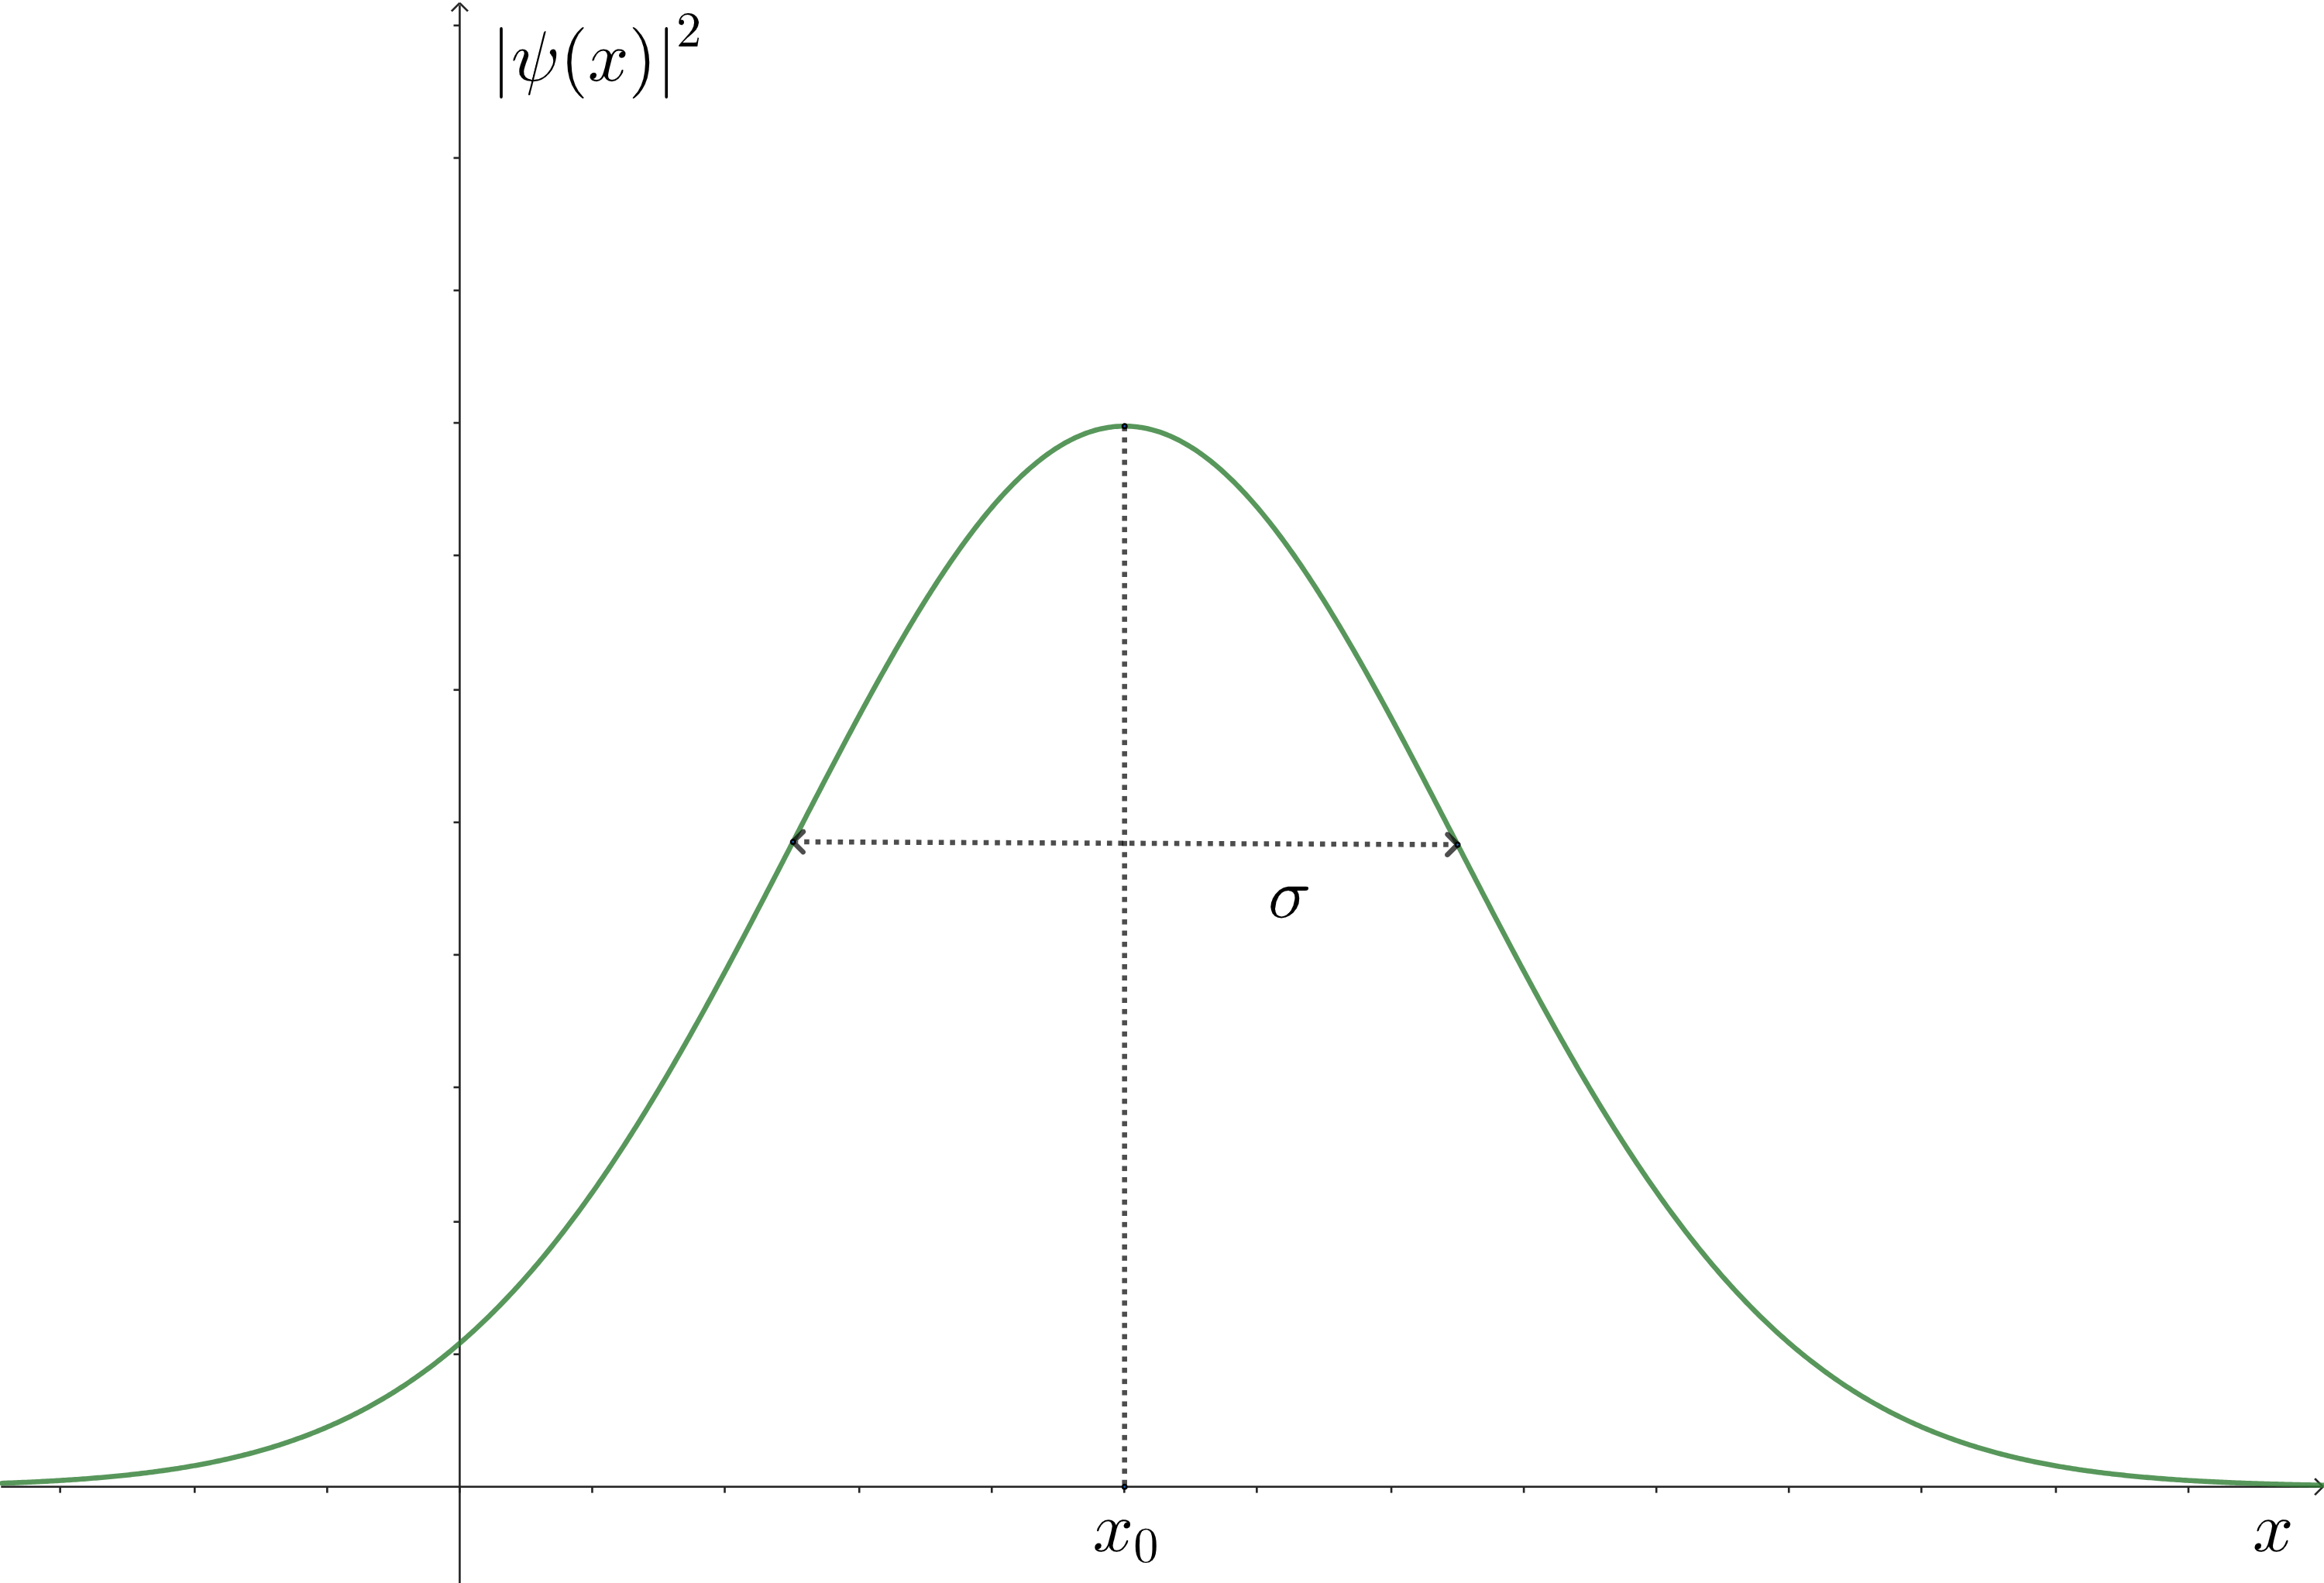
\includegraphics[scale = 3]{gaussian-wavepacket.png}
\end{center}
\par
Back to the use of Dirac notation, if we are give $\ketpsi \in \hilbert$, then
$$\brapsi = (\ketpsi)^{\dagger}$$
From the qubit system,
$$\ketpsi = \begin{pmatrix}
    \alpha \\ \beta
\end{pmatrix} \to \brapsi = \begin{pmatrix}
    \conj{\alpha} & \conj{\beta}
\end{pmatrix} = \conj{\alpha}\bra{0} + \conj{\beta}\bra{1}$$
From the 1D continuous system,
$$\ketpsi = \intR \psi(x)\ketx \dx \to \brapsi = \intR \conj{\psi}(x)\brax \dx$$
Then, given another quantum state in the discrete case:
$$\ketphi = \begin{pmatrix}
    \gamma \\ \zeta
\end{pmatrix}$$
We have
$$(\psi, \phi) = \conj{\alpha}\gamma + \conj{\beta}\zeta = \begin{pmatrix}
    \conj{\alpha} & \conj{\beta}
\end{pmatrix} \cdot \begin{pmatrix}
    \gamma \\ \zeta
\end{pmatrix} = \brapsi \cdot \ketphi = \braket{\psi}{\phi} = (\ketpsi, \ketphi)$$
In the continuous case, we have
$$(\psi, \phi) = \intR \conj{\psi}(x)\phi(x) \dx$$
Since the bra-ket notations are simply vectors, we also have the outer products between states, for example:
$$\dyad{0}{0} = \begin{pmatrix}
    1 \\ 0
\end{pmatrix} \begin{pmatrix}
    1 & 0
\end{pmatrix} = \begin{pmatrix}
    1 & 0 \\
    0 & 0
\end{pmatrix}$$
$$\dyad{\phi}{\psi} = \begin{pmatrix}
    \gamma \\ \zeta
\end{pmatrix}\begin{pmatrix}
    \conj{\alpha} & \conj{\beta}
\end{pmatrix} = \begin{pmatrix}
    \gamma\conj{\alpha} & \gamma\conj{\beta} \\
    \zeta\conj{\alpha} & \zeta\conj{\beta}
\end{pmatrix} \in \C^{2 \times 2}$$
% ----------------------------------------------------------------
\subsection{Postulate 3 - “公理”三}
After postulating the quantum system as a complex Hilbert space, with a quantum state being a normalized vector in this Hilbert space, we now wish to proceed to how to conduct a measurement on such a system, as we require measurement to obtain information. \par
In this case, we prepare a quantum system in state $\ketpsi \in \hilbert$, and let $\{\ket{x}\}_x$ to be an \impt{orthonormal basis} of $\hilbert$. From this setup, we know:
$$\braket{x}{x'} = \delta_{xx'} = \delta(x-x')$$
\begin{postulate}
    \raggedright
    A quantum system $\hilbert$ can be measured with respect to an orthonormal basis $\{\ket{x}\}_x$, such that the possible outcomes are labels $\{x\}_x$ with probability distribution/density
    $$ \Prob{x}_\psi = \abs{\braket{x}{\psi}}^2 $$
    This is also referred to as \uimpt{Born's Rule}. \\
    The post-measurement state upon receiving outcome $x$ is $\ket{x}$, this is equivalent to saying ``measurement changes the state'', or ``\uimpt{measurement corresponds to the collapse of the wavefunction}''
\end{postulate}
Note that a single quantum system can only produce a single outcome. If we wish to learn more about a state $\ketpsi$, we need multiple preparations and measurements to estimate $\Prob{x}_\psi$. \par
Now we wish to know, given an orthonormal basis $\{\ket{x}\}_x$ of the quantum system $\hilbert$, to which state will the wavefunction collapse?
\begin{definition}
    Quantum measurements with respect to an orthonormal basis are also called \uimpt{projective measurements}. Assume the orthonormal basis with resepct to which we are measuring is $\{\ket{x}\}_x$, we define a \uimpt{projector onto $\ket{x}$} to be:
    $$\proj{x} = \dyad{x}{x}$$
\end{definition}
We derive from Born's Rule:
\begin{align*}
    \Prob{x}_\psi &= \abs{\braket{x}{\psi}}^2 \\
    &= \braket{x}{\psi}^{*}\braket{x}{\psi} \\
    &= \braket{\psi}{x}\braket{x}{\psi} \\
    &= \mel{\psi}{\proj{x}}{\psi}
\end{align*}
If we wish to measure in another basis, we must represent the state in terms of the new basis first. This once again highlights that \impt{wavefunctions are dependent on the basis}. \par
In order for $\Prob{x}_\psi$ to be a probability distribution, two conditions must hold:
\begin{quote}
    1. $\Prob{x}_\psi \ge 0$ \\
    2. $\displaystyle \Sumi{x} \Prob{x}_\psi = 1$
\end{quote}
It is trivial that $\Prob{x}_\psi \ge 0$, as it is a complex number's norm's square. However, to satisfy the second condition, we require \impt{normalization}:
$$\Sumi{x} \Prob{x}_\psi = \Sumi{x} \abs{\braket{x}{\psi}}^2 = \Sumi{x} \abs{\psi(x)}^2 = 1$$
This derivation is natural from the fact that:
$$\ketpsi = \Sumi{x} \psi(x)\ket{x}$$
To deal with a continous Hilbert space, we may replace the summation symbol with the integral. \par
To a measurement, only the outcome and the probability of the outcome matter, therefore, \impt{global phases are physically irrelevant}. To show this, consider two quantum states where they only differ by a global phase $e^{\imag \varphi}$, that is, given:
$$\ketpsi \ne e^{\imag \varphi}\ketphi = \ketphi, \varphi \in \R, \text{ not a multiple of } 2\pi$$
If we wish to know the probability of outcome $x$ for the state $\ketphi$, we have:
\begin{align*}
    \Prob{x}_\phi &= \abs{\braket{x}{\phi}}^2 \\
    &= \abs{\mel{x}{e^{\imag \varphi}}{\psi}} \\
    &= \abs{e^{\imag \varphi}}^2 \abs{\braket{x}{\psi}}^2 \\
    &= \Prob{x}_\psi
\end{align*}
This derivation is natural because $e^{\imag \varphi}$ is a complex number with norm being $1$. \par
We may also describe the process of measurements in another way.
\begin{definition}
    An \uimpt{observable} $\mathcal{O}$ is a \uimpt{Hermitian operator}, where measuring $\mathcal{O}$ amounts to doing a \uimpt{projective measurement} with respect to the \uimpt{orthonormal basis of eigenvectors} of $\mathcal{O}$, and relabelling the outcome $x$ as $\lambda_x$
\end{definition}
Take a qubit as an example, a Pauli-Z measurement would amount to doing a projective measurement with respect to $\ket{0}$ and $\ket{1}$ as
$$Z = \begin{pmatrix}
    1 & 0 \\
    0 & -1
\end{pmatrix} = (+1)\begin{pmatrix}
    1 & 0 \\
    0 & 0
\end{pmatrix} + (-1) \begin{pmatrix}
    0 & 0 \\
    0 & 1
\end{pmatrix}$$
where $+1$ is the eigenvalue of eigenvector $\ket{0}$ and $-1$ is the eigenvalue of eigenvector $\ket{1}$. \\
Similarly, a Pauli-X measurement would amount to doing a projective measurement with respect to $\ketplus$ and $\ketminus$, with their respective eigenvalues to be $+1$ and $-1$. \\
In a continuous case, consider the position measurement as an example, where $\{\ket{x}\}_{x \in \R}$ is the position basis. We label $\lambda_x = x$, then the position observable is:
$$\oppos = \intR \lambda_x \dyad{x}{x} \dd x$$
\begin{definition}
    Given an observable $\mathcal{O}$ and a state $\ketpsi$, then the \uimpt{expected value} of this observable with respect to this state is:
    $$\expval{\mathcal{O}}_\psi = \ev{\mathcal{O}}{\psi}$$
\end{definition}
\begin{definition}
    The \uimpt{variance} of the above observable and the above state is:
    $$(\Delta \mathcal{O})_\psi^2 = \expval{\mathcal{O}^2}_\psi - (\expval{\mathcal{O}}_\psi)^2$$
\end{definition}
Once again, consider a general position state $\ketpsi = \intR \psi(x) \ket{x} \dd x$, and the above position observable. Then, the expected value of the position observable with respect to state $\ketpsi$ is:
\begin{align*}
    \expval{\oppos}_\psi &= \ev{\oppos}{\psi} \\
    &= \brapsi \intR x \dyad{x}{x} \dd x \ketpsi \\
    &= \intR x \dyad{\psi}{x}\dyad{x}{\psi} \dd x \\
    &= \intR x \conj{\psi}(x) \psi(x) \dd x \\
    &= \intR x \abs{\psi(x)}^2 \dd x
\end{align*}
We often wish to properly represent the outcome or the \impt{post-measurement} state. In this case, if we denote the initial state to be $\ketpsi$, and the post-measurement state to be $\ket{\psi'}$, then we have
$$\ket{\psi'} = \frac{\proj{i}\ketpsi}{\sqrt{\Prob{\lambda_i}}}$$
An additional useful operator is the \impt{reflection (parity)} operator, where we denote it as $\hat{R}$:
$$\hat{R} = \intR \dyad{x}{-x} \dd x$$
and has the following properties:
\begin{quote}
    1. $\hat{R}\ket{x} = \ket{-x}$. \\
    2. $\hat{R}^2 = \mathbb{I}$. \\
    3. $\hat{R}\oppos\hat{R} = -\oppos$
\end{quote}

\subsection{Postulate 4 - “公理”四}
So far, we have postulated the settings of a physical system in a quantum-mechanic way. We have defined a \impt{quantum system} in terms of a Hilbert space, a \impt{quantum state} in terms of a normalized vector in such a Hilbert space, and how the system can be \impt{measured} with respect to an orthonormal basis which relates to an \impt{observable} represented as a Hermitian operator. \par
Furthermore, we also hope describe how such a system evolves in time. This is, we wish to understand the \impt{dynamics} of a quantum system.
\begin{postulate}
    Closed quantum systems that do not have interactions with other quantum systems, evolve \uimpt{reversibly} and the \uimpt{reversible evolution} of a state $\ketpsi \in \hilbert$ is expressed as a \uimpt{unitary transformation}.
    $$\ketpsi \to \opuni \ketpsi, \opuni \in \opuni(\hilbert)$$
\end{postulate}
Here, since \hyperref[subsec:unitary]{\textcolor{cyan}{unitary matrices}} are invertible, we have $\opuni^{-1} = \conjt{\opuni}$ which implies a reversible evolution. \par
An example of such unitary operators is the Hadamard operator, the evolution under the Hadamard gate is as follows:
\begin{align*}
    H \ket{0} &= \frac{1}{\sqrt{2}} \begin{pmatrix}
        1 & 1 \\
        1 & -1
    \end{pmatrix} \begin{pmatrix}
        1 \\ 0
    \end{pmatrix} = \frac{1}{\sqrt{2}} \begin{pmatrix}
        1 \\ 1
    \end{pmatrix} = \ketplus \\
    H \ket{1} &= \ketminus \\
    H \ketplus &= \ket{0} \\
    H \ketminus &= \ket{1}
\end{align*}
It is easily seen that the Hadamard preserves the inner product as $\braket{0}{1} = \braket{+}{-} = 0$
\subsubsection{Schr\"odinger's Equation - 薛定谔方程}
Let $\ket{\psi(t)}$ be a \impt{time-dependent} state evolving \impt{unitarily} in a closed system. At time $t_0$, we denote the state as $\ket{\psi(t_0)}$ and after time continues to $t$, we have observed the evolution as such $\ket{\psi(t_0)} \mapsto \ket{\psi(t)}$. \par
We wish to understand what equation of motion governs the evolution. The evolution defines the equation of motion, while the equation of motion implies evolution. An \impt{equation of motion} is a differential equation in time defining the evolution. \par
\begin{definition}
    Let $\opuni(t, t_0)$ be an unitary operator that time-evolves an initial state at $t_0$: $\ket{\psi(t_0)}$ to the evolved state at $t$: $\ket{\psi(t)}$. We call such an operator the \uimpt{propagator}.
    $$\opuni(t, t_0)\ket{\psi(t_0)} = \ket{\psi(t)}$$
\end{definition}
With this setup, we now derive the Schr\"odinger's equation. \par
We take the time-derivative $\dd t$ of the state $\ket{\psi(t)}$:
\begin{align*}
    \pdv{t} \ket{\psi(t)} &= \lim_{\Delta \to 0} \frac{\ket{\psi(t + \Delta)} - \ket{\psi(t)}}{\Delta} \\
    &= \lim_{\Delta \to 0} \frac{\opuni(t+\Delta, t)\ket{\psi(t)} - \ket{\psi(t)}}{\Delta} \\
    &= (\lim_{\Delta \to 0} \frac{\opuni(t+\Delta, t) - \id}{\Delta})\ket{\psi(t)}
\end{align*}
For easier interpretation, we temporarily denote $\displaystyle G = \lim_{\Delta \to 0} \frac{\opuni(t+\Delta, t) - \id}{\Delta}$, which is a linear operator. So, we have $\pdv{t} \ket{\psi(t)} = G \ket{\psi(t)}$. \par
We first observe that $G$ is \impt{anti-Hermitian}, proven through the following:
\begin{align*}
    \pdv{t} \braket{\psi(t)} &= 0 \\
    (\pdv{t}\bra{\psi(t)})\ket{\psi(t)} + \bra{\psi(t)}(\pdv{t} \ket{\psi(t)}) &= 0 \\
    \ev{\conjt{G}}{\psi(t)} + \ev{G}{\psi(t)} &= 0 \\
    \conjt{G} + G &= 0
\end{align*}
We now have the equation of motion: $\pdv{t} \ket{\psi(t)} = G\ket{\psi(t)}$, where $G$ is anti-Hermitian. \par
By convention, we multiply the equation of motion by $\imag \hbar$. This would have the effect of $G \mapsto \imag G$ which is now Hermitian. In this case, we define the \impt{Hamiltonian} as 
$$\hat{H} := \imag \hbar G$$
Then, we finally obtain the \impt{time-dependent Schr\"odinger's equation}:
$$\hat{H}\ket{\psi(t)} = \imag \hbar \pdv{t} \ket{\psi(t)}$$
This is the \impt{equation of motion of quantum states in a closed system}. \par
Since $\hat{H}$ is Hermitian, it can be interpreted as an observable, the physical quantity measured when measuring observable $\hat{H}$ is the \impt{total energy of the quantum system}. In general, the Hamiltonian can be time-dependent, but mostly time-independent (which is, $\hat{H}(t) \equiv \hat{H}$). In order to know what Hamiltonian maps to what evolution/propagator $\opuni(t, t_0)$, we need to solve the Schr\"odinger's equation for different Hamiltonians.

\subsection{Postulate 5 - “公理”五}
\begin{postulate}
    Let $A$ and $B$ be quantum systems associated with $\hilbert: \hilbert_A, \hilbert_B$. The \uimpt{composite system} $AB$ is associated with the Hilbert space:
    $$\hilbert_{AB} = \hilbert_A \otimes \hilbert_B$$
\end{postulate}
Take 2 qubits as an example, where the composite quantum system is essentially $\C^2 \otimes \C^2$. Then, the notation of a state in this system can be:
$$\ket{0}_A \otimes \ket{0}_B = \ket{0} \otimes \ket{0} = \ket{0}_A\ket{0}_B = \ket{0}\ket{0} = \ket{00}_{AB} = \ket{00}$$
For the same composite quantum system, consider the following state:
$$\ket{\psi^{00}}_{AB} = \frac{1}{\sqrt{2}}(\ket{00} + \ket{11})$$
It is not possible to write the quantum state in the form of $\ketpsi_A \otimes \ketphi_B$ even though it is a valid state of the composite system.
\begin{definition}
    For all possible/valid states in a composite quantum system, we define the states that can be written as the tensor product of quantum states of component systems (e.g. $\ketpsi_A \otimes \ketphi_B$) as \uimpt{product states}, and those that cannot be written in such a form as \uimpt{entangled states}.
\end{definition}
If we have an orthonormal basis $\{\ket{k}_A\}_k$ on $\hilbert_A$ and $\{\ket{j}_B\}_j$ on $\hilbert_B$, then $\{\ket{k}_A\ket{j}_B\}_{(k, j)}$ is an orthonormal basis of $\hilbert_A \otimes \hilbert_B$. A general state of such a system can be represented as:
$$\ketpsi_{AB} = \Sumi{k, j}\psi(k, j)(\ket{k}_A \otimes \ket{j}_B)$$
$$\ketpsi_{AB} = \intR\intR \psi(x, y)(\ket{x} \otimes \ket{y}) \dd x \dd y$$
If $\dim \hilbert_A, \dim \hilbert_B < \infty$, then $\dim (\hilbert_A \otimes \hilbert_B) = \dim \hilbert_A \cdot \dim \hilbert_B$. \par
Consider a local linear operator $M_A$ on subsystem $\hilbert_A$, then the corresponding global operator on the composite system is:
$$M_{AB} = \Sumi{m} \alpha_m S_A^{(m)} \otimes T_B^{(m)}$$
Then for a generic state, we have
$$M_{AB}\ketpsi_{AB} = \Sumi{m} \alpha_m \Sumi{k, j} \psi(k, j)(S_A^{(m)} \ket{k}_A) \otimes (T_B^{(m)} \ket{j}_B)$$
This indicates that if subsystem $A$ undergoes a unitary evolution $\opuni_A$ while $B$ does not undergo any evolution, the evolution on $AB$ is unitary $\opuni_{AB} = \opuni_A \otimes \id_B$. However, the converse is not true, that is, if the entire system undergoes a generic unitary evolution ($\opuni_{AB} \in \opuni(\hilbert_A \otimes \hilbert_B)$), it does not imply that each subsystem undergoes a unitary evolution. \par
Furthermore, if we consider a local projective measurement, that is say, let $\{\proj{A}^{(k)}\}_k$ be projectors of local measurements on $A$, then the operator on $AB$ is thus: $\{\proj{A}^{(k) \otimes \id_B}\}_k$. Almost the same rules apply to composite systems when compared to a single system:
\begin{quote}
    1. Born's Rule: $\Prob{k_A}_{\psi_{AB}} = \brapsi_{AB} \proj{A}^{(k)} \otimes \id_B \ketpsi_{AB}$. \\
    2. Post-measurement state upon receiving outcome $k_A$: $\frac{\proj{A}^{(k)} \otimes \id_B \ketpsi_{AB}}{\sqrt{\Prob{k_A}_{\psi_{AB}}}}$
\end{quote}
An example operator on composite systems is the controlled-NOT gate (a.k.a CNOT). It works on 2 qubits, and it is an operator of the following form:
$$\text{CNOT} = \dyad{0}{0} \otimes \id + \dyad{1}{1} \otimes X$$
The gate takes in 2 qubits, the first one being the ``control'' and the second being the ``target''. Its function is to flip the target if the control is $1$. Thus, in general, the operator does the following operations:
\begin{quote}
    1. $\ket{00} \mapsto \ket{00}$ \\
    2. $\ket{01} \mapsto \ket{01}$ \\
    3. $\ket{10} \mapsto \ket{11}$ \\
    4. $\ket{11} \mapsto \ket{10}$
\end{quote}
Explicitly, the CNOT gate should be a $4 \times 4$ matrix of the following form:
$$\text{CNOT} = \begin{pmatrix}
    1 & 0 & 0 & 0 \\
    0 & 1 & 0 & 0 \\
    0 & 0 & 0 & 1 \\
    0 & 0 & 1 & 0
\end{pmatrix}$$

\subsection{Bloch Sphere - 布洛赫球面}
To start with this concept, we first introduce the basic single-qubit gates: Pauli-X, Pauli-Y, and Pauli-Z. The matrix form, given in the computational Z basis, are:
$$X = \begin{pmatrix}
    0 & 1 \\
    1 & 0
\end{pmatrix}, Y = \begin{pmatrix}
    0 & -\imag \\
    \imag & 0
\end{pmatrix}, Z = \begin{pmatrix}
    1 & 0 \\
    0 & -1
\end{pmatrix}$$
Any pure state of a qubit can be described and visualized as a \impt{point on a 3D sphere of radius 1}. This is demonstrated as follows. \par
First, any pure state of a single qubit can be written as:
$$\ketpsi = \alpha \ket{0} + \beta \ket{1}$$
with $\abs{\alpha}^2 + \abs{\beta}^2 = 1$. Represent the coefficients (a complex number) in product form: $\alpha = \abs{\alpha}e^{\imag \omega_1}, \beta = \abs{\beta}e^{\imag \omega_2}$. So we have:
\begin{align*}
    \ketpsi &= \alpha \ket{0} + \beta \ket{1} \\
    &= |\alpha|e^{\imag \omega_1}\ket{0} + \abs{\beta}e^{\imag \omega_2}\ket{1} \\
    &= \abs{\alpha}\ket{0} + \abs{\beta}e^{\imag (\omega_2 - \omega_1)}\ket{1}
\end{align*}
where $e^{-\imag \omega_1}$ is a global phase (it does not change the state), and $\phi = \omega_2 - \omega_1$ (the relative phase between two basis states). \par
Since we want to represent this state on the surface of the sphere, we use spherical coordinates where $\theta \in [0, \pi]$ and $\phi \in [0, 2\pi)$. \par
Right now, we have $\ketpsi = \abs{\alpha}\ket{0} + \abs{\beta}e^{\imag\phi}\ket{1}$. We wish to justify that this state can be written as
$$\ketpsi = \cos(\frac{\theta}{2})\ket{0} + \sin(\frac{\theta}{2})e^{\imag \phi}\ket{1}$$
so that we can use $\theta$ and $\phi$ for spherical-coordinate representation. \par
So far, with $\ketpsi$ being a quantum state, it is trivial to see that we can easily denote $\abs{\alpha}$ as $\cos(x)$ and $\abs{\beta}$ as $\sin(x)$. Thus, we need to justify why $x$ here must be $\frac{\theta}{2}$ instead of some other value. We should start by considering what mathematical conditions $\abs{\alpha}$ and $\abs{\beta}$ should satisfy:
\begin{quote}
    1. $0 \le \abs{\alpha}, \abs{\beta} \le 1$. \\
    2. $\abs{\alpha}, \abs{\beta}$ should uniquely correspond to a $\theta$.
\end{quote}
This indicates that $\cos(x), \sin(x)$ must be within the range $0$ to $1$ while $x \in [0, \pi]$. This condition shows that if $x$ is a factor of $\theta$, the factor must be exactly $\frac{1}{2}$. Thus, we can properly justify why $\abs{\alpha} = \cos(\frac{\theta}{2})$ and $\abs{\beta} = \sin(\frac{\theta}{2})$. \par
Therefore, now when we consider the eigenstates (computational basis) of the Pauli-Z, -X, -Y operators on this Bloch sphere, we can see why the operators are named this way:
\begin{quote}
    1. Pauli-Z: has computational basis $\ket{0}$ and $\ket{1}$.
    $$\ket{0} = (\theta = 0, \phi); \ket{1} = (\theta = \pi, \phi)$$
    we see that $\ket{0}$ lies on the positive $z$-direction, and $\ket{1}$ lies on the negative $z$-direction; \\
    2. Pauli-X: has computational basis $\ketplus$ and $\ketminus$.
    $$\ketplus = (\theta = \frac{\pi}{2}, \phi = 0); \ketminus = (\theta = \frac{\pi}{2}, \phi = \pi)$$
    we see that $\ketplus$ lies on the positive $x$-direction, and $\ketminus$ lies on the negative $x$-direction; \\
    3. Pauli-Y: has computational basis $\ket{+\imag}$ and $\ket{-\imag}$.
    $$\ket{+\imag} = (\theta = \frac{\pi}{2}, \phi = \frac{\pi}{2}); \ket{-\imag} = (\theta = \frac{\pi}{2}, \phi = \frac{3\pi}{2})$$
    we see that $\ket{+\imag}$ lies on the positive $y$-direction, and $\ket{-\imag}$ lies on the negative $y$-direction.
\end{quote}
\begin{center}
    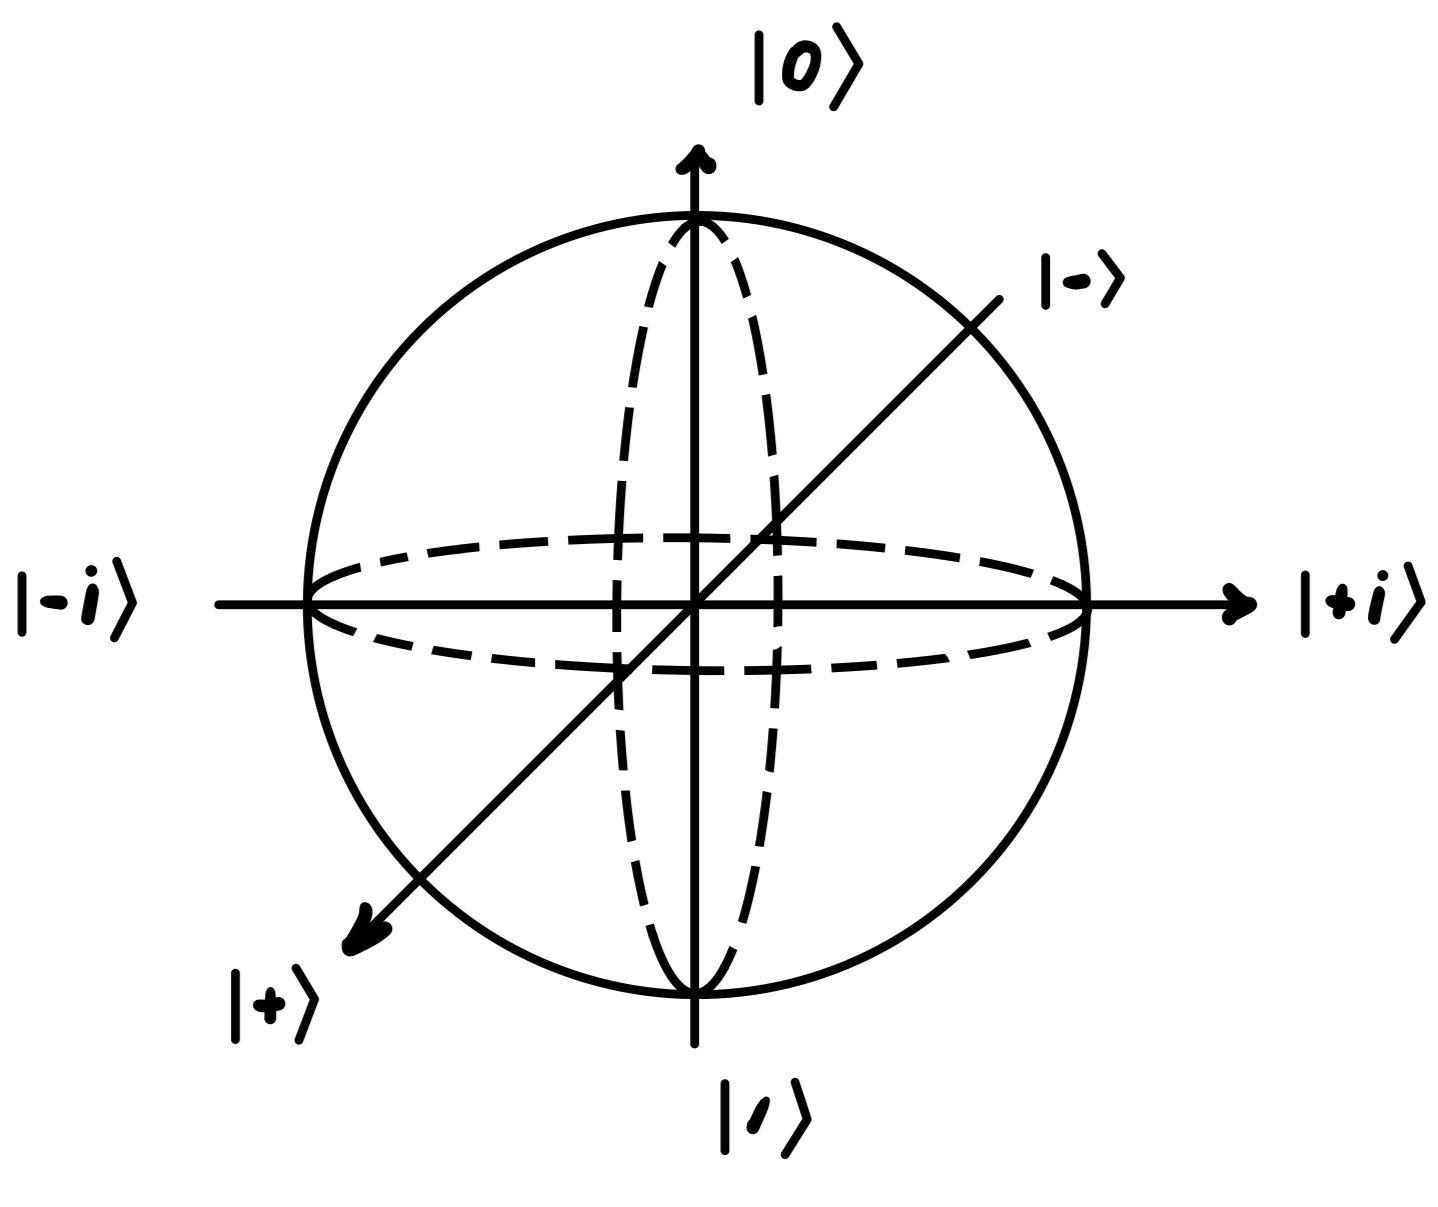
\includegraphics[scale = 0.25]{bloch-sphere.png}
\end{center}
It is helpful to know the following relationship:
\begin{align*}
    \ketpsi &= \alpha \ket{0} + \beta \ket{1} \\
    &= \frac{\alpha + \beta}{\sqrt{2}}\ketplus + \frac{\alpha - \beta}{\sqrt{2}}\ketminus
\end{align*}

\newpage
\section{Uniform Dynamics - 均匀动力演化}
From the time-dependent Schr\"odinger's Equation, it induces unitary evolution in a quantum system (which in converse, derives the Schr\"odinger's Equation), which is described by a unitary propagator in the form:
$$\opuni(t_2, t_1) \ket{\psi(t_1)} = \ket{\psi(t_2)}$$
\begin{definition}
    \uimpt{Uniform dynamics} is a term that describes unitary evolution. \\
    A unitary evolution is \uimpt{uniform} if
    $$\forall t_1, t_2, \opuni(t_2, t_1) = \opuni(t_2 - t_1, 0)$$
    i.e. the propagator only depends on the time difference $\Delta t= t_2 - t_1$
\end{definition}
Notation-wise, if an evolution is uniform, we write:
$$\opuni(t_2, t_1) = \opuni(t_2 - t_1)$$
\begin{theorem}
    A unitary evolution is uniform if and only if the associated Hamiltonian is time-independent ($\hamiltonian(t) \equiv \hamiltonian$).
\end{theorem}
Intuitively, if we start at the time-dependent Schr\"odinger's Equation, we should have:
\begin{align*}
    \imag \hbar \pdv{t}\ket{\psi(t)} &= \hamiltonian(t) \ket{\psi(t)} \\
    \pdv{t} \ket{\psi(t)} &= \frac{1}{\imag \hbar} \hamiltonian(t) \ket{\psi(t)} \\
    \Delta \ket{\psi(t)} & \approx \Delta t \cdot \frac{1}{\imag \hbar} \hamiltonian(t) \ket{\psi(t)}
\end{align*}
Then, if we wish that the evolution of the state is only dependent on the time difference ($\Delta t$), the Hamiltonian should be time-independent.
\subsection{Proof of Uniform Dynamics associates with a Time-independent Hamiltonian}
We first observe the following for uniform dynamics:
$$\opuni(\Delta t)\opuni(\Delta s)\ket{\psi(t)} = \opuni(\Delta t)\ket{\psi(t + \Delta s)} = \ket{\psi(t + \Delta s + \Delta t)} = \opuni(\Delta s + \Delta t)\ket{\psi(t)}$$
This gives the lemma
\begin{lemma}
    Let $\opuni(\cdot)$ be uniform, then
    $$\forall \ket{\psi(t)}\in\hilbert, \opuni(\Delta t)\opuni(\Delta s) = \opuni(\Delta t + \Delta s)$$
\end{lemma}
This gives us
$$\opuni(\Delta t)\opuni(\Delta t)\dots\opuni(\Delta t) = \opuni(\Delta t)^m = \opuni(m\cdot \Delta t)$$
Since $\opuni$ has some orthonormal eigenbasis $\{\ket{k}\}_k$, we know $\opuni^m$ has the \impt{same} orthonormal eigenbasis, and it remains same for all $m \in \N, \Delta t \in \R$. This thus shows the eigenbasis of $\opuni$ is independent of $\Delta t$, remains constant over time. Hence, we can express $\opuni(\Delta t)$ as the following forms:
\begin{align*}
    \opuni(\Delta t) &= \Sumi{k} \lambda_k(\Delta t) \dyad{k} \\
    &= \Sumi{k} e^{\imag \alpha_k(\Delta t)} \dyad{k}
\end{align*}
Since, we have $\opuni(\Delta t)^m = \opuni(m\cdot \Delta t)$, we have:
\begin{align*}
    \Sumi{k}(e^{\imag \alpha_k(\Delta t)})^m \dyad{k} &= \Sumi{k} e^{\imag \alpha_k(m\Delta t)} \dyad{k} \\
    m \cdot \alpha_k(\Delta t) &= \alpha_k(m \Delta t)
\end{align*}
This immediately shows that $\alpha_k$ is linear, and we can write it in the form of:
$$\alpha_k(\Delta t) = -\omega_k \cdot \Delta t$$
At this intermediate step, suppose that the initial state is an eigenstate of $\opuni(\Delta t)$, that is $\ket{\psi(0)} = \ket{k}$, then we must have:
$$\ket{\psi(t)} = \opuni(t)\ket{\psi(0)} = \Sumi{l}e^{\imag \alpha_l(t)}\dyad{l} \ket{k} = e^{\imag \alpha_k(t)}\ket{k} = e^{-\imag \omega_k t}\ket{k}$$
Notice that with respect to the initial state, it has only evolved with a global phase, that is $\abs{e^{-\imag \omega_k t}} = 1$, the direction of the state remains unchanged.
\begin{definition}
    Quantum states that only evolve with a global phase are \uimpt{stationary states}.
\end{definition}
However, even though stationary states only evolve with a global phase, for each state, there will be a different $\omega_k$ that essentially determines the angular velocity at which it ``rotates''. \par
We then insert this intermediate conclusion into the Schr\"odinger's Equation with a general $\hamiltonian(t)$:
\begin{align*}
    \hamiltonian(t)\ket{\psi(t)} &= \imag \hbar \pdv{t}\ket{\psi(t)} \\
    \hamiltonian(t)(e^{-\imag \omega_k t}\ket{k}) &= \imag \hbar \pdv{t}(e^{-\imag \omega_k t}\ket{k}) \\
    e^{-\imag \omega_k t}\hamiltonian(t)\ket{k} &= \imag \hbar (-\imag \omega_k)(e^{-\imag \omega_k t}\ket{k}) \\
    \hamiltonian(t)\ket{k} &= \hbar \omega_k \ket{k}
\end{align*}
We can thus conclude that:
\begin{quote}
    1. The eigenstates of $\opuni(\Delta t)$ are also eigenstates of the Hamiltonian. \\
    2. The eigenvalues of $\hamiltonian(t)$ are $\hbar \omega_k =: E_k$, which are constant.
\end{quote}
With these two conclusions, we finally can claim that $\hamiltonian(t)$ is a constant operator independent of time:
$$\hamiltonian(t) \equiv \hamiltonian \equiv \Sumi{k}E_k\dyad{k}$$

\subsection{Proof of Time-independent Hamiltonian reflects Uniform Dynamics}
If the Hamiltonian is time-independent, we can write the Hamiltonian in the form:
$$\hamiltonian = \Sumi{k}E_k \dyad{k}$$
where $\{\ket{k}\}_k$ is the orthonormal eigenbasis of the Hamiltonian. \par
Consider an arbitrary state, expressed in this basis, we have:
$$\ket{\psi(t)} = \Sumi{k}c_k(t) \ket{k}$$
Then, the Schr\"odinger's Equation implies:
\begin{align*}
    \hamiltonian\ket{\psi(t)} &= \imag \hbar \pdv{t}\ket{\psi(t)} \\
    \hamiltonian (\Sumi{k}c_k(t) \ket{k}) &= \imag \hbar \pdv{t}(\Sumi{k}c_k(t) \ket{k}) \\
    \Sumi{k}c_k(t) \hamiltonian \ket{k} &= \imag \hbar \Sumi{k}c_k^{'}(t) \ket{k} \\
    \Sumi{k}c_k(t) E_k \ket{k} &= \Sumi{k} \imag \hbar c_k^{'}(t) \ket{k}
\end{align*}
Component-wise, with each summand, we have:
$$c_k(t) E_k = \imag \hbar c_k^{'}(t)$$
which is a differential equation with the solution:
$$c_k(t) = C_k^{(0)}\exp(\frac{E_k t}{\imag \hbar}) = C_k^{(0)}\exp(-\imag \frac{E_k t}{\hbar})$$
where $C_k^{(0)}$ is the initial condition. \par
Here, we know the time evolution of an arbitrary state under the time-independent Hamiltonian:
$$\ket{\psi(t)} = \Sumi{k} C_k^{(0)}\exp(-\imag \frac{E_k t}{\hbar}) \ket{k}$$
We choose the unitary propagator of this time evolution to be:
$$\opuni(\Delta t) = \Sumi{k} e^{-\imag \omega_k t}\dyad{k}$$
where $\omega_k = \frac{E_k}{\hbar}$, this propagator is uniform by design. We then show that this indeed is the desired propagator.
\begin{align*}
    \opuni(\Delta t)\ket{\psi(t)} &= (\Sumi{l} \exp(-\imag \omega_l \Delta t) \dyad{l})(\Sumi{k} C_k^{(0)}\exp(-\imag \omega_k t) \ket{k}) \\
    &= \Sumi{k} C_k^{(0)} \exp(-\imag \omega_k (t + \Delta t)) \ket{k} \\
    &= \ket{\psi(t+\Delta t)}
\end{align*}
In a continuous space, we also have:
\begin{align*}
    \opuni(\Delta t)\ket{\psi(t)} &= \intR \exp(-\imag \omega_y \Delta t) \dyad{y} \dd y \intR C_k^{(0)} \exp(-\imag \omega_x t) \ket{x} \dd x \\
    &= \intR\intR C_k^{(0)} \exp(-\imag \omega_x t) \exp(-\imag \omega_y \Delta t) \ket{y}\braket{y}{x} \dd x \dd y \\
    &= \intR C_k^{(0)} \exp(-\imag \omega_x t) \exp(-\imag \omega_x \Delta t) \ket{x} \dd x \\
    &= \ket{\psi(t+\Delta t)}
\end{align*}

\subsection{Intermediate Summary}
To summarize, for uniform dynamics, the Schr\"odinger's Equation is reduced to the eigenvalue problem:
$$\hamiltonian\ket{k} = E_k \ket{k}$$
which is also the \impt{time-independent Schr\"odinger's Equation}. After solving the eigenvalue problem, we will be able to find $\{E_k\}_k$ and $\{\ket{k}\}_k$. \par
We would also know the unitary propagator to be:
$$\opuni(\Delta t) = \Sumi{k} e^{-\imag \omega_k t}\dyad{k}$$
where $\omega_k = \frac{E_k}{\hbar}$, and the eigenstates of the propagator are \impt{stationary states}:
$$\opuni(t)\ket{k} = e^{-\imag \omega_k t}\ket{k}$$
And, for an arbitrary state, the time evolution is:
$$\ket{\psi(t)} = \Sumi{k} C_k^{(0)}\exp(-\imag \omega_k t) \ket{k}$$

\subsection{Rotation on the Bloch Sphere - 量子态在布洛赫球面的旋转}
Consider an example of a Hamiltonian being the following:
$$\hamiltonian = EX = \begin{pmatrix}
    0 & E \\
    E & 0
\end{pmatrix}$$
where $E \in \R$, and the eigenbasis of the Hamiltonian is the same as that of Pauli-X: $\{\ketplus, \ketminus\}$. We know that
$$X = \dyad{+} - \dyad{-}$$
then, we have
$$\hamiltonian = (+E)\ketbra{+}{+} + (-E)\ketbra{-}{-}$$
Recall that for uniform dynamics, if $\displaystyle \hamiltonian = \Sumi{k}E_k \dyad{k}$, then the unitary propagator is represented by $\displaystyle \opuni(t) = \Sumi{k}e^{-\imag \omega_k t} \dyad{k}$, where $\omega_k = \frac{E_k}{\hbar}$. Thus, in this case, the unitary propagator is:
$$\opuni(t) = \exp(-\imag \frac{E}{\hbar} t)\dyad{+} + \exp(\imag \frac{E}{\hbar} t)\dyad{-}$$
Suppose the initial state $\ket{\psi(0)} = \ket{0} = \frac{\ketplus + \ketminus}{\sqrt{2}}$, we have:
\begin{align*}
    \ket{\psi(t)} &= \frac{1}{\sqrt{2}}(\exp(-\imag \frac{E}{\hbar} t)\ketplus + \exp(\imag \frac{E}{\hbar} t)\ketminus) \\
    &= \cos(\frac{Et}{\hbar})\ket{0} - \imag \cdot \sin(\frac{Et}{\hbar})\ket{1}
\end{align*}
The evolution reflects the rotation in the Bloch sphere around the axis through the eigenbasis of $\hamiltonian$, which in this case $\{\ketplus, \ketminus\}$
\begin{center}
    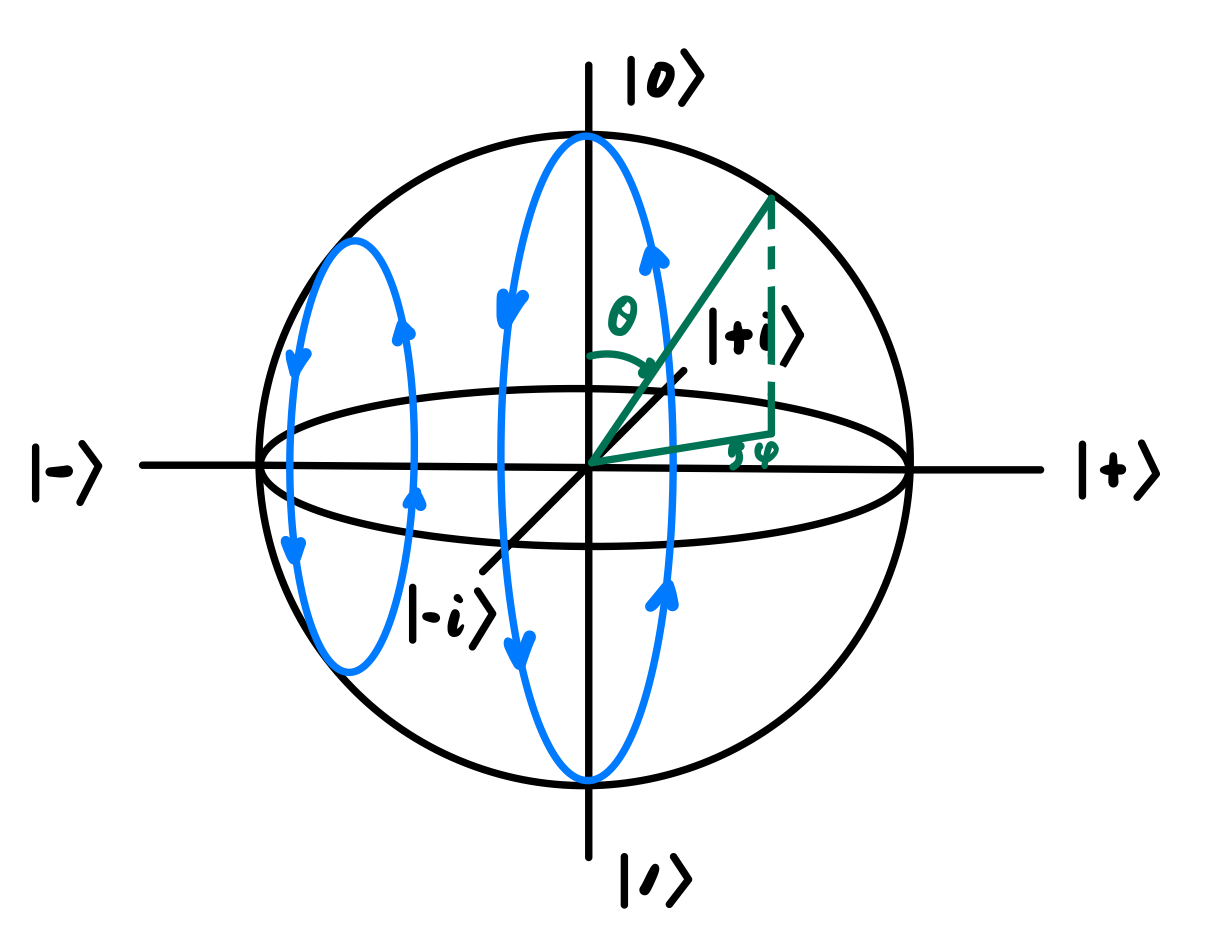
\includegraphics[scale = 0.3]{bloch-sphere-rotation.png}
\end{center}
We may also substitute Pauli-X with other Pauli operators so that the rotation would be in the respective axis.

\subsection{Evolution of Observables and Symmetries - 可观测量的演化和对称性}
From the third postulate, we know for a time-independent observable $A$, which is a Hermitian operator, the expected value of $A$ is:
$$\expval{A}_\psi = \expval{A}{\psi}$$
From this, we wish to understand how does $\expval{A}$ evolve with respect to $\psi$ evolving in time.
\begin{definition}
    Consider an observable $A$ with respect to a state $\ketpsi$, the evolution of this observable in time is
    $$\expval{A}_t := \expval{A}_{\psi(t)} = \expval{A}{\psi(t)}$$
\end{definition}
This further means $\expval{A}_t = \expval{\conjt{\opuni(t)}A\opuni(t)}{\psi(0)}$. \par
Knowing how $\ket{\psi(t)}$ evolves from the fourth postulate, we can look into the time-derivative of the expected value of an observable $A$ over time with respect to a state $\ketpsi$:
\begin{align*}
    \pdv{t} \expval{A}_t &= \pdv{t} \expval{A}{\psi(t)} \\
    &= \bra{\psi(t)}A(\pdv{t}\ket{\psi(t)}) + (\pdv{t}\bra{\psi(t)})A\ket{\psi(t)} \\
    &= \bra{\psi(t)}A(-\frac{\imag}{\hbar} \hamiltonian \ket{\psi(t)}) + (\frac{\imag}{\hbar} \bra{\psi(t)} \conjt{\hamiltonian})A\ket{\psi(t)} \\
    &= \frac{\imag}{\hbar}(\expval{-A\hamiltonian}{\psi(t)} + \expval{\hamiltonian A}{\psi(t)}) \\
    &= \frac{\imag}{\hbar} \expval{\hamiltonian A-A\hamiltonian}{\psi(t)} \\
    &= \frac{\imag}{\hbar} \expval{[\hamiltonian, A]}_t
\end{align*}
\begin{definition}
    An observable $A$ is called a \uimpt{conserved quantity} if
    $$\pdv{t} \expval{A}_t = 0$$
\end{definition}
Equivalently, this means, for time-independent observables $A$, $A$ is \impt{conserved} $\iff$ for all time $t$, $A$ \hyperref[subsec:commutator]{\textcolor{cyan}{commutes with}} $\hamiltonian$, that is, $[\hamiltonian, A] = 0$. Here, a time-independent observable means the projective measurement is independent of time, or, the state is always measured in the same way regardless of time evolution. \par
A trivial example is that $[\hamiltonian, \hamiltonian] = 0$, where as we previously reached that $\hamiltonian$ can be interpreted as an observable such that when measured reflects the total energy of the system, meaning \impt{total energy of a system is conserved}.
\begin{definition}
    A unitary operator $V$ is called a \uimpt{symmetry} if it commutes with the unitary propagator for all times, that is,
    $$[V, \opuni(t)] = 0$$
\end{definition}
Conserved quantities and symmetries imply each other.

\newpage
\section{Stern--Gerlach Experiment - 施特恩--格拉赫实验}
This experiment demonstrated that the magnetic moments (a.k.a spins of the electrons) of silver atoms are quantized (that is, it is not a classical degree of freedom).

\subsection{Setup - 实验设置}
\begin{center}
    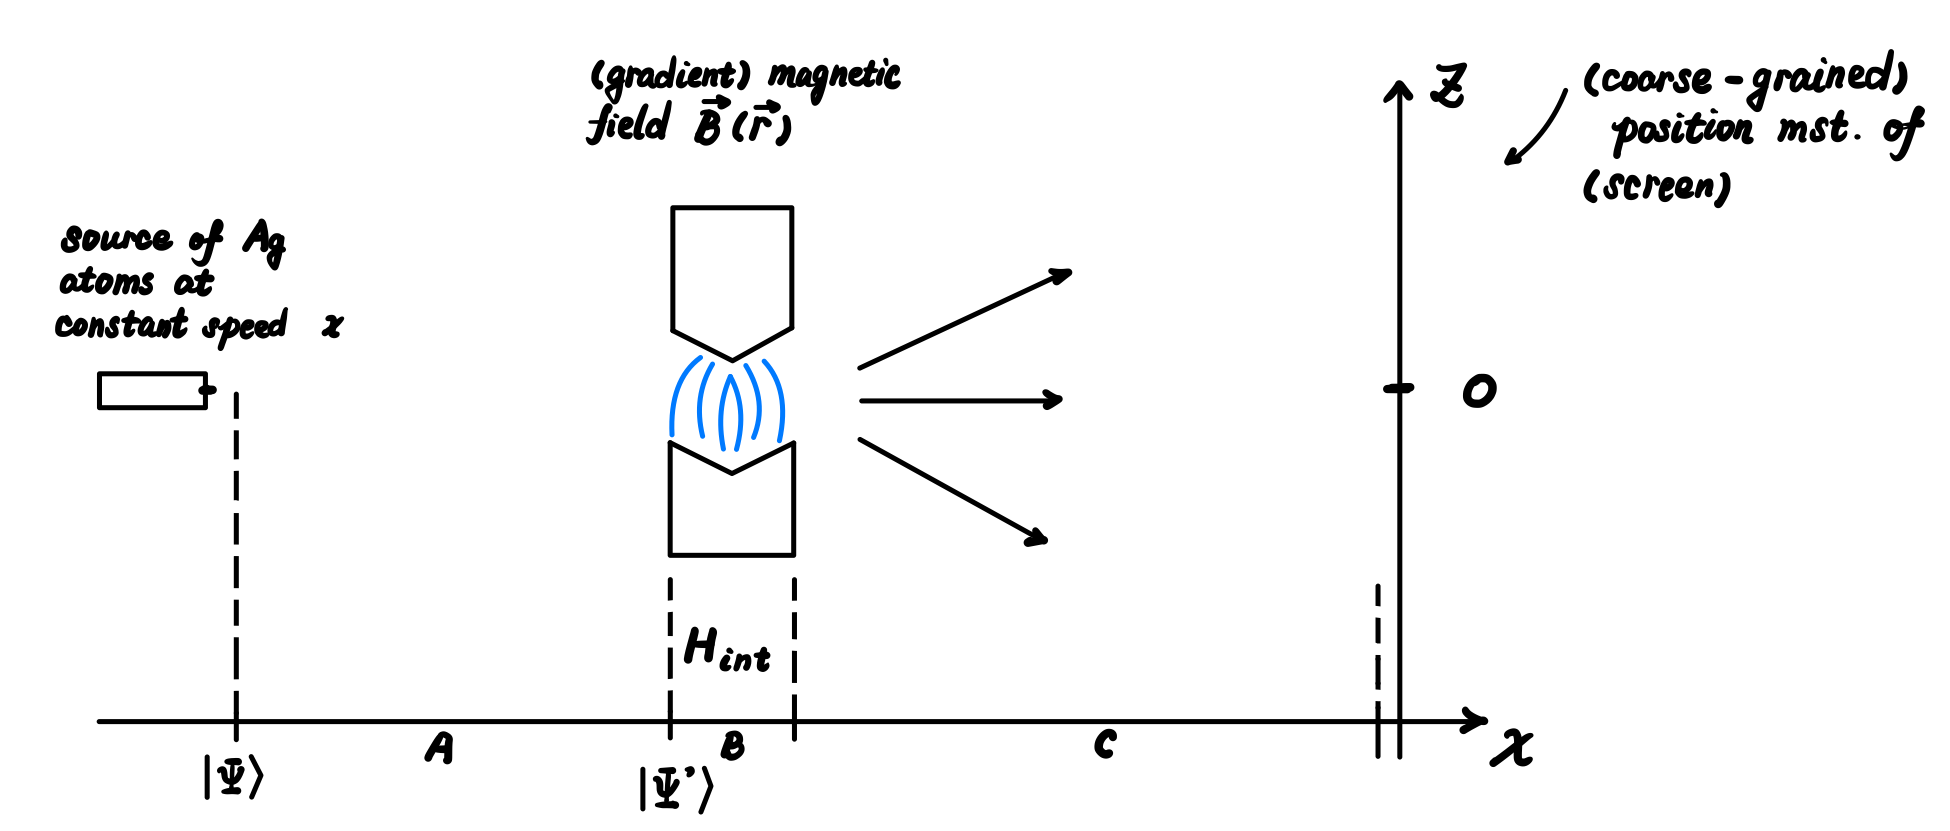
\includegraphics[scale = 0.45]{stern-gerlach-setup.png}
\end{center}
We set up the experiment such that the silver atoms are emitted at a constant speed along the $x$-axis. It will pass through a magnetic field and we observe where it lands on a coarse-grained screen.

\subsection{A First Look - 实验浅尝}
A first look of the experiment assumes that in region $A$ and $C$, the Hamiltonian will be $\hamiltonian = 0$, while in region $B$, the region of interaction, we denote it as $\hamiltonian_{\text{int}}$. We also assume that the speed at emittance remains constant throughout, so the position along the $x$-axis is proportional to time: $x(t) \propto t$. \par
Since we know the Hamiltonian, when viewed as an observable, when measured yields the energy of the total system, so in the interaction region, we have the Hamiltonian to be:
$$\hamiltonian_{\text{int}} = -\vec{\mu} \cdot \vec{B}(\vec{r})$$
where $\vec{\mu}$ is the magnetic moment, $\vec{B}$ is the magnetic field. Here, we approximate the magnetic field is only along the $z$-axis, and the magnetic moment is along the $z$-axis in a Bloch sphere. So the interaction Hamiltonian becomes:
$$\hamiltonian_{\text{int}} = -\mu_z \cdot B_z(\vec{r})$$
If we analyze the experiment classically, the force exerted on the silver atom in the magnetic field should be:
$$\vec{F} = -\nabla\hamiltonian_{\text{int}} = \begin{pmatrix}
    0 \\ 0 \\
    \mu_z \pdv{B_z(\vec{r})}{z}
\end{pmatrix}$$
where the force in $z$-direction should depend on the magnetic moment. Thus, the classical expectation yields that, assuming the magnetic moments in $z$-direction are classical degrees of freedom and they are random from source, the distribution of silver atoms observed on the screen should spread out from the center with the center having the largest density (Gaussian distribution). However, actual observation indicates that the center of the screen has little to none observations but there are two peaks on at positions $+\Delta$ and $-\Delta$. \par
The classical explanation fails to reflect the observation, thus, we need to explain this phenomenon in a quantum model. \par
To start with, we model the quantum system as:
$$\hilbert_{\text{total}} = \hilbert_{\text{magnetic}} \otimes \hilbert_z$$
where $\hilbert_{\text{mag}}$ is spanned by $\{\ket{0}, \ket{1}\}$ ($\ket{0}$ denotes spinning upwards, and $\ket{1}$ denotes spinning downwards), and $\hilbert_z$ is spanned by $\{\ket{z}\}_z$ (a 1D continuous position space). Here, the $x$-direction and $y$-direction are not modelled, as they do not contribute to our analysis. \par
The initial state can thus be modelled as the following:
$$\ketPsi = (\alpha \ket{0} + \beta \ket{1}) \otimes \ketpsi_z$$
where
$$\ketpsi_z = \intR \psi(z)\ket{z} \dd z$$
and $\abs{\psi(z)}^2 \propto -\frac{z^2}{2\sigma^2}$ (a Gaussian random variable). \par
From here on, we wish to understand the evolution of the state. \par
It is trivial to observe that in regions where $\hamiltonian = 0$, the state remains constant as Schr\"odinger's equation demonstrates that the time-derivative of the state is $0$. \par
For the interaction region, classically, we have shown what it is previously. However, in a quantum model, the classical quantities must be promoted to operators/observables:
\begin{align*}
    \hilbert_{\text{int}} &= - (\gamma Z \otimes \id) \cdot (\id \otimes B_z(\vec{r})) \\
    &= -\gamma Z \otimes B_z(\vec{r})
\end{align*}
The corresponding unitary evolution operator will have the following mapping:
$$\opuni: \begin{cases}
    \ket{0} \otimes \ketpsi \mapsto \ket{0} \otimes \mathcal{T}_{+\Delta}\ketpsi \\
    \ket{1} \otimes \ketpsi \mapsto \ket{1} \otimes \mathcal{T}_{-\Delta}\ketpsi
\end{cases}$$
where $\mathcal{T}$ is the translation operator and the subscript is how much the operator translates the state on the $z$-direction. \par
This means, the evolution leads to a magnetic-moment-dependent shift of particle in $\pm \Delta$, where the size of $\Delta$ depends on the strength of $\vec{\mu}, \vec{B}$ and $\nabla\vec{B}$. We assume deflection by $\Delta$ to be visible: $\Delta >> \sigma$. \par
Now, on the final state after evolution, we perform a local position measurement in the $z$-direction. This means, on the magnetic moment space, the operator is $\id_{\text{mag}}$. Since the observation occurs on a coarse-grained screen, we can assume finite precision $\varepsilon > 0$, where the screen can be evenly spaced out by regions of size $\varepsilon$. The projector on the entire state will be:
$$\id \otimes \int_{n\varepsilon}^{(n+1)\varepsilon} \dyad{z} \dd z$$
where $n \in \Z$. Random magnetic moment means random $\alpha, \beta$.

\subsection{Preparation for a Deeper Analysis - 深度分析准备}
With the same setup, we can then consider the 3 dimensional case. Define the Hilbert space to be $\hilbert = \hilbert_x \otimes \hilbert_y \otimes \hilbert_z$. This can be expressed in two ways:
$$\hilbert = \Span{\ket{\vec{r}}}_{\vec{r} \in \R^3} = \Span{\ket{\vec{p}}}_{\vec{p} \in \R^3}$$
where
$$\vec{r} = \begin{pmatrix}
    x \\ y \\ z
\end{pmatrix}, \ket{\vec{r}} = \ket{xyz}; \vec{p} = \begin{pmatrix}
    p_x \\ p_y \\ p_z
\end{pmatrix}, \ket{\vec{p}} = \ket{p_xp_yp_z}$$
The inner product between the two basis state is:
\begin{align*}
    \braket{\vec{r}}{\vec{p}} &= (\bra{x} \otimes \bra{y} \otimes \bra{z})(\ket{p_x} \otimes \ket{p_y} \otimes \ket{p_z}) \\
    &= (2\pi\hbar)^{-\frac{3}{2}} \exp(\frac{\imag \vec{r} \cdot \vec{p}}{\hbar})
\end{align*}
A general state, can also be expressed in two ways:
$$\ketpsi = \int_{\R^3} \psi(\vec{r})\ket{\vec{r}} \dd^3 \vec{r} = \int_{\R^3} \tilde{\psi}(\vec{p})\ket{\vec{p}}\dd^3 \vec{p}$$
The relevant operators/observables are defined as follows:
$$\oppos = \oppos \otimes \id_y \otimes \id_z, \opmtm_x = \opmtm_x \otimes \id_y \otimes \id_z, \dots$$
where the operators act on the wavefunctions in these ways:
\begin{align*}
    \oppos&: \begin{cases}
        \psi(\vec{r}) \mapsto x\psi(\vec{r}) \\
        \tilde{\psi}(\vec{p}) \mapsto \imag \hbar \pdv{p_x}\tilde{\psi}(\vec{p})
    \end{cases} \\
    \opmtm_y&: \begin{cases}
        \psi(\vec{r}) \mapsto -\imag \hbar \pdv{y}\psi(\vec{r}) \\
        \tilde{\psi}(\vec{p}) \mapsto p_y\tilde{\psi}(\vec{p})
    \end{cases}
\end{align*}
Consequently, we consider two vectors of operators being:
$$\opmtm = \begin{pmatrix}
    \opmtm_x \\ \opmtm_y \opmtm_z
\end{pmatrix}, \hat{R} = \begin{pmatrix}
    \oppos \\ \hat{Y} \\ \hat{Z}
\end{pmatrix}$$
where $\hat{R}^2 = \oppos^2 + \hat{Y}^2 + \hat{Z}^2$, and when $\opmtm^2$ is applied to $\psi(\vec{r})$, we have:
$$\opmtm^2: \psi(\vec{r}) \mapsto -\hbar^2 \nabla^2 \psi(\vec{r})$$
The key commutators are:
$$[\oppos, \opmtm_x] = [\hat{Y}, \opmtm_y] = [\hat{Z}, \opmtm_z] = \imag \hbar \id_x \otimes \id_y \otimes \id_z$$

\subsection{Deeper Analysis - 深度分析}
We model the quantum system with $\hilbert = \hilbert_s \otimes \hilbert_x \otimes \hilbert_z$, where $\hilbert_s = \Span{\ket{0}, \ket{1}}$ and the other two are the corresponding position spaces. The Hamiltonian will be in two parts:
$$\hamiltonian_{sxz} = \hamiltonian_0 + \hamiltonian_{\text{interaction}}$$
where $\hamiltonian_0 = \frac{1}{2\mu}(\opmtm_x^2 + \opmtm_z^2)$, the interaction Hamiltonian should model the magnetic field:
$$\hamiltonian_{\text{int}} = \gamma \cdot Z \otimes \proj{x}^{[0, \delta]} \otimes \hat{Z}$$
This is essentially derived from $\hamiltonian_{\text{int}} = -\vec{\mu} \cdot \vec{B}$. For spin-$\frac{1}{2}$ atoms:
$$\vec{\mu} \propto \begin{pmatrix}
    X \otimes \id \otimes \id \\
    Y \otimes \id \otimes \id \\
    Z \otimes \id \otimes \id
\end{pmatrix}$$
and the magnetic field is a gradient in spatial $z$-direction and only non-zero for $x \in [0, \delta]$, so:
$$\vec{B}(\hat{R}) \propto \begin{pmatrix}
    0 \\ 0 \\
    \id \otimes \proj{x}^{[0, \delta]} \otimes \hat{Z}
\end{pmatrix}$$
Thus, when multiplied together, we have $\hamiltonian_{\text{int}}$, where $\gamma$ is dependent on the magnetic field strength, coupling constant of the spin to the magnetic field. \par
With the Hilbert space set up, we can have the initial state to be:
$$\ketPsi_{sxz} = (\alpha \ket{0} + \beta \ket{1}) \otimes \ket{\psi_0}_{xz}$$
with the initial position wavefunction to be:
$$\psi_0(x, z) = (\frac{1}{\sqrt[4]{2\pi\sigma^2}})^2\exp(-\frac{(x-x_0)^2}{4\sigma^2}-\frac{(z-z_0)^2}{4\sigma^2}+\imag k x)$$
This represents a Gaussian wavepacket in the $x,z$ directions and an initial momentum in $x$ direction travelling from left to right.
\begin{center}
    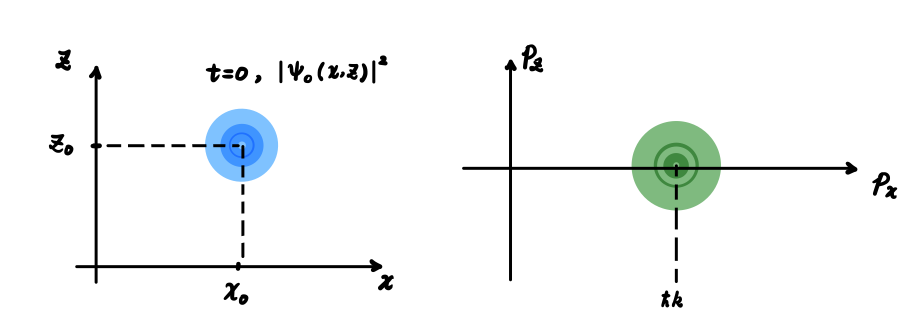
\includegraphics[scale = 1]{stern-gerlach-initial.png}
\end{center}
The time evolution is hard to solve because the unitary propagator is:
$$\opuni(t) = \exp(-\frac{\imag t}{\hbar}(\hamiltonian_0 + \hamiltonian_{\text{int}}))$$
where $\exp(A+B) \ne \exp(A) + \exp(B)$ if $[A, B] \ne 0$. \par
We can first conduct a semi-classical analysis separately per region. For regions $A, C$, the \impt{support} (the part of function that is only larger than $\varepsilon$) of the position wavefunction
$$\text{supp}_\varepsilon(\psi_{xz}) \cap [0, \delta] \approx \varnothing$$
We then can approximate:
$$\hamiltonian_{\text{int}} \ketPsi \approx 0 \to \opuni_{AC}(t) \approx \exp(-\frac{\imag t}{\hbar}\hamiltonian_0) = \id \otimes \exp(-\frac{\imag t}{2\mu\hbar}\opmtm_x^2) \otimes \exp(-\frac{\imag t}{2\mu\hbar}\opmtm_z^2)$$
With the Ehrenfest Relations in \hyperref[subsec:ehrenfest]{\textcolor{cyan}{Section 5.2}}, we have two sets of relationship:
\begin{align*}
    \expval{\oppos}_t &= \expval{\oppos}_0 + t \cdot \frac{\expval{\opmtm_x}_0}{\mu} = x_0 + t \cdot \frac{\hbar k}{\mu} \\
    \expval{\opmtm_x}_t &= \expval{\opmtm_x}_0= \hbar k \\
    (\Delta \oppos)_t^2 &= \sigma^2 + \frac{\hbar^2}{4\sigma^2\mu^2} \cdot t^2 \\
    (\Delta \opmtm_x)_t^2 &= \frac{\hbar^2}{4\sigma^2} \\
    \expval{\hat{Z}}_t &= \expval{\hat{Z}}_0 + t \cdot \frac{\expval{\opmtm_z}_0}{\mu} = z_0 \\
    \expval{\opmtm_z}_t &= \expval{\opmtm_z}_0= 0 \\
    (\Delta \hat{Z})_t^2 &= \sigma^2 + \frac{\hbar^2}{4\sigma^2\mu^2} \cdot t^2 \\
    (\Delta \opmtm_z)_t^2 &= \frac{\hbar^2}{4\sigma^2}
\end{align*}
\begin{center}
    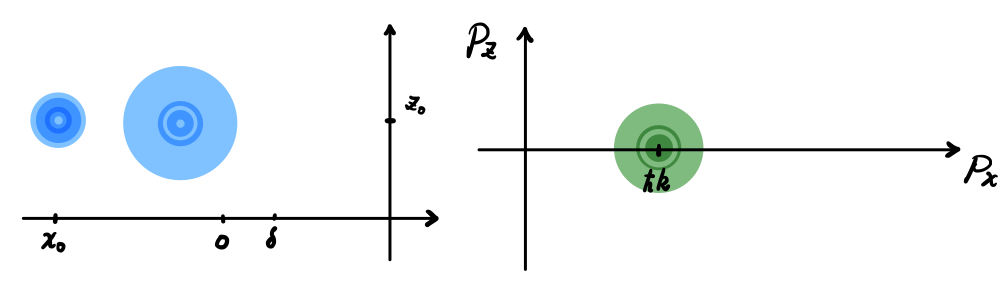
\includegraphics[scale = 0.8]{stern-gerlach-nonint.png}
\end{center}
For region $B$, we can assume a strong magnetic field and strong coupling to approximate $\hamiltonian$ to be $\hamiltonian_{\text{int}}$ only.
\begin{lemma}
    Consider an operator $A$ and a projector $\Pi$, we have
    $$e^{A \otimes \Pi} = e^A \otimes \Pi + \id \otimes (\id - \Pi)$$
\end{lemma}
So the unitary propagator is:
$$\opuni_B(t)_{szx} \approx \exp(-\frac{\imag t}{\hbar} \hamiltonian_{\text{int}}) = \exp(-\frac{\imag t \gamma}{\hbar}(Z \otimes \hat{Z})) \otimes \proj{x}^{[0, \delta]} + (\id \otimes \id) \otimes (\id - \proj{x}^{[0, \delta]})$$
We specifically need to investigate how $\exp(-\frac{\imag t \gamma}{\hbar}(Z \otimes \hat{Z}))$ acts on $\hilbert_s \otimes \hilbert_z$. Consider an arbitrary state $\ketPhi_{sz} = (\alpha \ket{0} + \beta \ket{1}) \otimes \ketphi_z$, this operator yields:
\begin{align*}
    \exp(-\frac{\imag t \gamma}{\hbar}(Z \otimes \hat{Z})) \ketPhi_{sz} &= \alpha\exp(-\frac{\imag t \gamma}{\hbar}(Z \otimes \hat{Z})) \ket{0}\ket{\phi} \\
    &+ \beta\exp(-\frac{\imag t \gamma}{\hbar}(Z \otimes \hat{Z})) \ket{1}\ket{\phi}
\end{align*}
Through mathematical manipulation (skipped here), we finally have:
$$\alpha \ket{0} \otimes \exp(-\frac{\imag t \gamma}{\hbar}\hat{Z})\ketphi_z + \beta \ket{1} \otimes \exp(+\frac{\imag t \gamma}{\hbar}\hat{Z})\ketphi_z$$
We then investigate the behaviour of: $\exp(\pm\frac{\imag t \gamma}{\hbar}\hat{Z})$.
\begin{align*}
    \psi(z) &\mapsto \exp(\pm \frac{\imag t \gamma}{\hbar}z)\phi(z) \\
    \tilde{\psi}(p_z) &\mapsto \tilde{\psi}(p \pm t\gamma)
\end{align*}
where the second relation is conducted through Fourier transform.
\begin{center}
    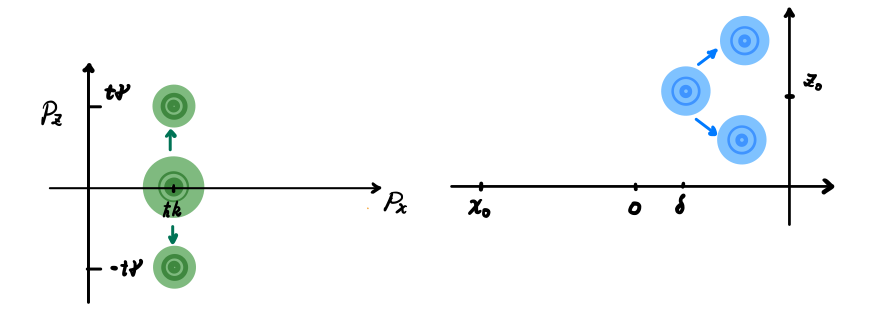
\includegraphics[scale = 1]{stern-gerlach-int.png}
\end{center}
When the wavepacket reached the screen, the state will be:
$$\ket{\Psi'}_{sxz} = \alpha\ket{0}_s \otimes \ket{\psi_+}_{xz} + \beta\ket{1}_s \otimes \ket{\psi_-}_{xz}$$
Finally, when we conduct a position measurement with the projectors to be: $\{\proj{n\varepsilon}\}_{n \in \Z - \{0\}}$, where each projector is:
$$\proj{n\varepsilon} = \id \otimes \id \otimes \int_{n\varepsilon}^{(n+1)\varepsilon} \dyad{z} \dd z$$
The probability is thus:
\begin{align*}
    \Prob{n} &= \expval{\proj{n\varepsilon}}{\Psi'} \\
    &= \abs{\alpha}^2 \cdot \intR \int_{n\varepsilon}^{(n+1)\varepsilon} \abs{\psi_+(x, z)}^2 \dd z \dd x \\
    &+ \abs{\beta}^2 \cdot \intR \int_{n\varepsilon}^{(n+1)\varepsilon} \abs{\psi_-(x, z)}^2 \dd z \dd x
\end{align*}
The post-measurment state is thus:
$$\frac{\proj{n\varepsilon}\ket{\Psi'}_{sxz}}{\sqrt{\Prob{n}}}$$
\begin{center}
    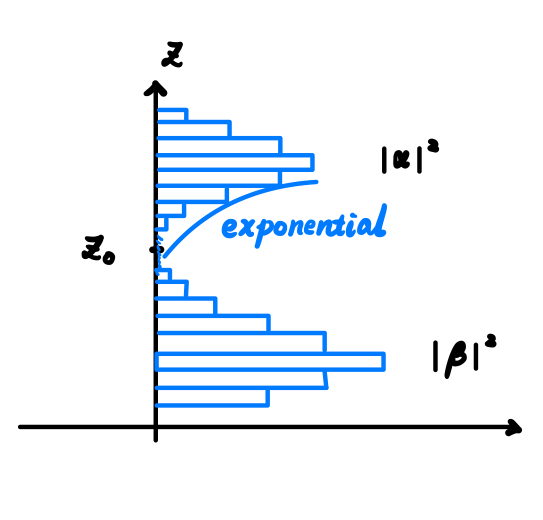
\includegraphics[scale = 0.5]{stern-gerlach-outcome.png}
\end{center}

\newpage
\section{Position and Momentum Observables - 位置与动量可观测量}
\subsection{The Properties of and Transformations between the Observables - 可观测量的性质和互相变换}
In this section, we explore the relationship between the two important observables. \\
First, we revisit the 1D continuous system, where the quantum system is defined as a Hilbert space: $\hilbert = \Span{\ket{x}}_{x \in \R}$ with the condition $\braket{x}{x'} = \delta(x-x')$. A general quantum state can be expressed in the position basis:
$$\ketpsi = \intR \psi(x)\ketx \dd x, \intR \abs{\psi(x)}^2 \dd x = 1$$
where in particular we know $\psi(x) = \braket{x}{\psi}$. \\
We have the \impt{position observable} to be:
$$\oppos = \intR x \dyad{x} \dd x$$
However, we can also represent the same state in another basis, say $\ket{p}_{p \in \R}$. Here, a general state will be represented as:
$$\ketpsi = \intR \tilde{\psi}(p) \ket{p} \dd p, \tilde{\psi}(p) = \braket{p}{\psi}$$
We now wish to understand how the position wavefunction and the momentum wavefunction relate with each other. Here, we may substitute the state in different bases in the wavefunction calculation:
\begin{align*}
    \psi(x) &= \braket{x}{\psi} \\
    &= \brax \intR \tilde{\psi}(p) \ket{p} \dd p \\
    &= \intR \tilde{\psi}(p) \braket{x}{p} \dd p \\
    \tilde{\psi}(p) &= \intR \psi(x) \braket{p}{x} \dd x
\end{align*}
We observe that, knowing the inner product between these two bases is enough to properly build the relationship.
\begin{definition}
    Define $\ket{p}_{p \in \R}$ to be the \uimpt{momentum basis} in an 1D continuous system, where the inner product between the position basis and the momentum basis is:
    $$\forall x, p \in \R, \braket{x}{p} = \frac{1}{\sqrt{2\pi\hbar}}\exp(\frac{\imag p x}{\hbar})$$
\end{definition}
Therefore,
\begin{align*}
    \psi(x) &= \frac{1}{\sqrt{2\pi\hbar}} \intR \tilde{\psi}(p) \exp(\frac{\imag p x}{\hbar}) \dd p \\
    \tilde{\psi}(p) &= \frac{1}{\sqrt{2\pi\hbar}} \intR \psi(x) \exp(-\frac{\imag p x}{\hbar}) \dd x
\end{align*}
They represent the \impt{Fourier transform} between the two bases. \\
We can thus further express a basis state in the other basis as follows:
\begin{align*}
    \ketx &= \id \ketx \\
    &= \intR \dyad{p} \dd p \ketx \\
    &= \intR \ket{p}\braket{p}{x} \dd p \\
    &= \frac{1}{\sqrt{2\pi\hbar}} \intR \exp(-\frac{\imag p x}{\hbar}) \ket{p} \dd p \\
    \ket{p} &= \frac{1}{\sqrt{2\pi\hbar}} \intR \exp(\frac{\imag p x}{\hbar}) \ket{x} \dd x
\end{align*}
This can be confirmed by the above definition being consistent with the Dirac delta function $\braket{x}{x'} = \delta(x-x')$ even expressing $\ketx$ in the momentum basis. The deduction process is hereby not shown.
\begin{definition}
    Define the momentum observable to be:
    $$\hat{P} = \intR p \dyad{p} \dd p$$
    where it has the property of being Hermitian: $\conjt{\hat{P}} = \hat{P}$
\end{definition}
It is straightforward to understand that when the observables act on the respective wavefunction of respective basis, we have:
$$\begin{cases}
    \hat{X}: \psi(x) \mapsto x \cdot \psi(x) \\
    \hat{P}: \tilde{\psi}(p) \mapsto p \cdot \tilde{\psi}(p)
\end{cases}$$
However, we wish to further know how the observables act on each other's wavefunction. One way is to calculate $\psi(x)$ after $\hat{P}$ is applied:
\begin{align*}
    \mel{x}{\hat{P}}{\psi} &= \brax (\intR p \dyad{p} \dd p) \ketpsi \\
    &= \intR p \braket{x}{p}\braket{p}{\psi} \dd p \\
    &= \frac{1}{\sqrt{2 \pi \hbar}} \intR p \cdot \exp(\frac{\imag p x}{\hbar}) \tilde{\psi}(p) \dd p
\end{align*}
The key here is to notice that: $p \cdot \exp(\frac{\imag p x}{\hbar}) = (-\imag \hbar)\pdv{x}\exp(\frac{\imag p x}{\hbar})$. Notice that the partial derivative and the integral are both linear, thus, we can swap their positions and have:
\begin{align*}
    \mel{x}{\hat{P}}{\psi} &= -\imag \hbar \pdv{x} \intR \frac{1}{\sqrt{2 \pi \hbar}} \exp(\frac{\imag p x}{\hbar}) \tilde{\psi}(p) \dd p \\
    &= -\imag \hbar \pdv{x} \psi(x)
\end{align*}
Therefore, we yield:
$$\begin{cases}
    \hat{X}: \tilde{\psi}(p) \mapsto +\imag \hbar \pdv{p}\tilde{\psi}(p) \\
    \hat{P}: \psi(x) \mapsto -\imag \hbar \pdv{x}\psi(x)
\end{cases}$$
Finally, we wish to observe how the two observables commute. We first have:
\begin{align*}
    \mel{x}{\hat{X}\hat{P}}{\psi} &= (\brax \hat{X})(\hat{P} \ketpsi) \\
    &= x\mel{x}{\hat{P}}{\psi} \\
    &= x \cdot (-\imag \hbar \pdv{x} \psi(x))
\end{align*}
Then, we also have:
\begin{align*}
    \mel{x}{\hat{P}\hat{X}}{\psi} &= (\brax \hat{P})(\hat{X} \ketpsi) \\
    &= \mel{x}{\hat{P}}{(x \cdot \psi(x))} \\
    &= -\imag \hbar \pdv{x} (x \cdot \psi(x)) \\
    &= -\imag \hbar \psi(x) - \imag \hbar x \cdot \pdv{x}\psi(x)
\end{align*}
So, we must have:
$$\mel{x}{[\hat{X}, \hat{P}]}{\psi} = \mel{x}{\hat{X}\hat{P}}{\psi} - \mel{x}{\hat{P}\hat{X}}{\psi} = \imag \hbar \psi(x)$$
This eventually gives us
\begin{theorem}
    $$[\hat{X}, \hat{P}] = \imag \hbar \id$$
\end{theorem}

\subsection{Ehrenfest Relations - 埃伦费斯特原理}
\label{subsec:ehrenfest}
So far, we can understand the action of operators as one of the following:
\begin{quote}
    1. Representation of the action itself \\
    2. Provides eigenvectors and eigenvalues \\
    3. Its action on coefficients of vectors in a specific basis
\end{quote}
We have previously shown the canonical commutation relation between the position and momentum observables. Now we wish to utilize this knowledge to connect the classical representations and the quantum representations. \\
Consider a neutral particle in an 1D continuous space. \impt{Classically}, we may express the total energy $E$ in this classical system by the sum of the particle's kinetic energy $E_k = \frac{1}{2}\mu \cdot v^2 = \frac{p^2}{2\mu}$ and the particle's potential energy $E_p = V(x)$, where the position $x$ is a function of time $x(t)$ and the momentum is also a function of time $p(t)$. The equation of motion are derived to be:
$$\pdv{t}x(t) = \frac{p(t)}{\mu}, \pdv{t}p(t) = -\pdv{V(x(t))}{x}$$
In the quantum world, classical physical variables, as shown in the Stern-Gerlach experiment, are promoted to observables/operators. In this case:
\begin{quote}
    1. Total Energy: $\hamiltonian$. \\
    2. Position: $\hat{X}$. \\
    3. Momentum: $\hat{P}$.
\end{quote}
where the Hamiltonian is:
$$\hamiltonian = \frac{\opmtm^2}{2\mu} + V(\oppos)$$
and we assume that $V$ has a Taylor expansion, where
$$V(\oppos) = \Sum{n=0}{\infty}a_n \oppos^n$$
Recall that for a time-independent observable, we have
$$\pdv{t}\expval{\hat{A}}_t = \frac{\imag}{\hbar} \expval{[\hamiltonian, \hat{A}]}_t$$
This gives us:
\begin{align*}
    \pdv{t}\expval{\oppos}_t &= \frac{\imag}{\hbar} \expval{[\frac{\opmtm^2}{2\mu} + V(\oppos), \oppos]}_t \\
    &= \frac{\imag}{\hbar} \expval{[\frac{\opmtm^2}{2\mu}, \oppos] + [V(\oppos), \oppos]}_t \\
    &= \frac{\imag}{2\mu \hbar} \expval{[\opmtm^2, \oppos]}_t
\end{align*}
Specifically, we have
\begin{align*}
    [\opmtm^2, \oppos] &= \opmtm\opmtm\oppos - \oppos\opmtm\opmtm \\
    &= \opmtm(\oppos\opmtm - [\oppos, \opmtm]) - \oppos\opmtm\opmtm \\
    &= -\opmtm[\oppos, \opmtm] + \opmtm\oppos\opmtm - \oppos\opmtm\opmtm \\
    &= -\imag \hbar \opmtm + ([\opmtm, \oppos])\opmtm \\
    &= -2\imag\hbar\opmtm
\end{align*}
Therefore,
\begin{align*}
    \pdv{t}\expval{\oppos}_t &= \frac{\imag}{2\mu \hbar} \expval{[\opmtm^2, \oppos]}_t \\
    &= \frac{\imag}{2\mu \hbar} \expval{-2\imag\hbar\opmtm}_t \\
    &= \frac{\expval{\opmtm}_t}{\mu}
\end{align*}
In a similar fashion, we have:
\begin{align*}
    \pdv{t}\expval{\opmtm}_t &= \frac{\imag}{\hbar} \expval{[\frac{\opmtm^2}{2\mu} + V(\oppos), \opmtm]}_t \\
    &= \frac{\imag}{\hbar} \expval{[V(\oppos), \opmtm]}_t \\
    &= \frac{\imag}{\hbar} \expval{\imag\hbar \pdv{V(\oppos)}{x}}_t \\
    &= -\expval{\pdv{V(\oppos)}{x}}_t
\end{align*}
This concludes that:
\begin{theorem}
    The \uimpt{Ehrenfest Relations/Theorem} claims that for a neutral particle in an 1D continuous system, we have an analagous relationship between classical physical quantities and their promoted observables, specifically:
    $$\pdv{t}\expval{\oppos}_t = \frac{\expval{\opmtm}_t}{\mu}$$
    $$ \pdv{t}\expval{\opmtm}_t =  -\expval{\pdv{V(\oppos)}{x}}_t$$
\end{theorem}
In this case, we further explore how the Schr\"odinger's Equation is affected for such a particle. \\
For vectors, we already have the Schr\"odinger's Equation to be:
$$\hamiltonian \ket{\psi(t)} = \imag \hbar \pdv{t}\ket{\psi(t)}$$
The position wavefunction is thus transformed in the following way (by applying $\brax$ from the left):
\begin{align*}
    \forall x \in \R, \mel{x}{\hamiltonian}{\psi(t)} &= \mel{x}{\imag \hbar \pdv{t}}{\psi(t)} \\
    &= \imag\hbar \pdv{t}\braket{x}{\psi(t)} \\
    &= \imag \hbar \pdv{t}\psi(x, t)
\end{align*}
If we further separate the Hamiltonian in its respective parts, we first have:
\begin{align*}
    \frac{\opmtm^2}{2\mu}: \psi(x, t) &\mapsto \frac{1}{2\mu}(-\imag\hbar\pdv{x})^2 = -\frac{\hbar^2}{2\mu}\pdv[2]{x} \psi(x, t) \\
    V(\oppos): \psi(x, t) &\mapsto V(x)\psi(x, t)
\end{align*}
Therefore, 
\begin{theorem}
    For a neutral particle in 1D-continous space, we have two Schr\"odinger's Equation, one for position, and one for momentum:
    \begin{align*}
        -\frac{\hbar^2}{2\mu}\pdv[2]{x} \psi(x, t) + V(x)\psi(x, t) &= \imag \hbar \pdv{t}\psi(x, t) \\
        \frac{p^2}{2\mu}\tilde{\psi}(p, t) + V(\imag \hbar \pdv{p})\tilde{\psi}(p, t) &= \imag \hbar \pdv{t}\tilde{\psi}(p, t)
    \end{align*}
\end{theorem}
If we have solutions for $\psi(x, t)$ and $\tilde{\psi}(p, t)$, then we know that
$$\ket{\psi(t)} = \intR \psi(x, t) \ket{x} \dd x = \intR \tilde{\psi}(p,t) \ket{p} \dd p$$
is a solution for the Schr\"odinger's Equation for $\ket{\psi(t)}$. \\
To simply demonstrate, consider a free particle where $V(x) = 0$, so the Hamiltonian is directly $\hamiltonian = \frac{\opmtm^2}{2\mu}$. We know that $\opmtm^2 = \intR p^2 \dyad{p} \dd p$ is diagonal in the momentum basis, so it is easier for us to solve the equation for $\tilde{\psi}(p, t)$.
\begin{align*}
    \frac{p^2}{2\mu}\tilde{\psi}(p, t) &= \imag \hbar \pdv{t}\tilde{\psi}(p, t) \\
    -\frac{\imag p^2}{2\mu\hbar} \tilde{\psi}(p, t) &= \pdv{t} \tilde{\psi}(p, t) \\
    \tilde{\psi}(p, t) &= \tilde{\psi}(p, 0) \cdot \exp(-\frac{\imag p^2t}{2\mu\hbar})
\end{align*}
Thus, the equation of motion for a general state $\ket{\psi(t)}$ is:
$$\ket{\psi(t)} = \intR \tilde{\psi}(p, 0) \cdot \exp(-\frac{\imag p^2t}{2\mu\hbar}) \ket{p} \dd p$$
The consistency can be checked with the propagator:
$$\opuni(t) = \exp(-\frac{\imag \hamiltonian t}{\hbar})$$
applied to $\ket{\psi(0)} = \intR \tilde{\psi}(p, 0) \ket{p} \dd p$. \\
By the Ehrenfest relations, we also know
$$\pdv{t} \expval{\opmtm}_t = - \expval{\pdv{V(\oppos)}{x}}_t = 0$$
This indicates the momentum is conserved, which further implies:
$$\pdv{t} \expval{\oppos}_t = \frac{\expval{\opmtm}_t}{\mu} = \frac{\expval{\opmtm}_0}{\mu}$$
which is equivalent to $\expval{\oppos}_t = \expval{\oppos}_0 + t \cdot \frac{\expval{\opmtm}_0}{\mu}$. \\
In this case, $(\Delta \oppos)_t \propto t^2$. On a similar note, we yielded that the momentum wavefunction is transformed in the following way:
$$\tilde{\psi}(p, t) = \tilde{\psi}(p, 0) \cdot \exp(-\frac{\imag p^2t}{2\mu\hbar})$$
We can observe it only evolves with a complex phase. This indicates that every moment of $\opmtm$, which is $\expval{\opmtm^n}_t$ is time-independent. In momentum space, this does not change much, but in position space, it changes the wavefunction significantly, more specifically, the probability spreads out as time evolves.

\newpage
\section{Particles in an 1D Potential - 一维空间具有势能的粒子运动}
From the prevous section, we have the Hamiltonian of a particle in 1D continous space to be:
$$\hamiltonian = \frac{\opmtm^2}{2\mu} + V(\oppos)$$
Our goal now is to solve many Schr\"odinger's Equations with different $V(x)$. We primarily focus on using the time-independent Schr\"odinger's Equation related to the position wavefunction:
$$-\frac{\hbar^2}{2\mu}\pdv[2]{x} \psi(x, t) + V(x)\psi(x, t) = E \psi(x, t)$$

\subsection{Particle in a Box - 闭盒中的粒子}
We start with a special case, where the potential energy as a function of position is defined as follows:
$$V(x) = \begin{cases}
    0, & x \in [0, L] \\
    \infty, & \text{otherwise}
\end{cases}$$
The boundary conditions include:
\begin{quote}
    1. For $x$ outside the box, the potential energy is positive infinity, meaning the particle cannot be outside, as it has $0$ probability of being measured. This translates to:
    $$\forall t, \forall x \notin [0, L], \psi(x, t) = 0$$
    2. We want at least a continuous wavefunction, which means:
    $$\forall t, \psi(0, t) = \psi(L, t) = 0$$
\end{quote}
This thus gives us two parts:
$$\begin{cases}
    x \in [0, L]: & -\frac{\hbar^2}{2\mu}\pdv[2]{x} \psi(x, t) = E \psi(x, t) \\
    x \notin [0, L]: & -\frac{\hbar^2}{2\mu}\pdv[2]{x} \psi(x, t) + V(x)\psi(x, t) = E \psi(x, t)
\end{cases}$$
where in the second case, $V(x)\psi(x, t) = 0$. \\
We solve for $\psi(x)$ and $E$. It is claimed that for this equation, we have the wavefunction to be:
$$\psi_n(x) = \begin{cases}
    A\sin(k_n x), & x \in [0, L] \\
    0, & x \notin [0, L]
\end{cases}$$
and we solve the equation for $n = 1, 2, 3, \dots$ with
$$k_n = \frac{\pi n}{L}, E_n = \frac{\hbar^2 k_n^2}{2\mu} = \frac{\hbar^2 \pi^2 n^2}{2L^2 \mu} = E_1 \cdot n^2$$
These can be easily checked by substituting the relevant factors into the equation. More importantly, the normalization factor $A$ can be obtained by:
\begin{align*}
    \int_{0}^{L} \abs{\psi_n(x)}^2 \dd x &= 1 \\
    A &= \sqrt{\frac{2}{L}}
\end{align*}
For the time evolution, we can consider an arbitrary state like $\ket{\psi(0)} = \frac{1}{\sqrt{2}}(\ket{\psi_l} + \ket{\psi_m})$, and observe its time evolution to find out the wavefunction's evolution. \\
From this particle in a box calculation, we observe that:
\begin{quote}
    1. The energy spectrum and the solution to the Schr\"odinger's Equation is ``quantized'' (i.e. discrete, not continuous). An energy measurement ($\hamiltonian$ observable) can only give discrete outcomes like $E_1, E_2, \dots$. \\
    2. Formally, the quantization comes from the boundary condition where $\psi(0) = \psi(L) = 0$.
\end{quote}

\subsection{Continuity Conditions - 波函数连续性条件}
From the Schr\"odinger's equation, consider the part $-\frac{\hbar^2}{2\mu}\pdv[2]{x} \psi(x)$, we expect that $\psi \in C^2$, that is twice-differentiable and continuous. However, if we magnify at the boundary, depending on the potential chosen, a twice-differentiable and continuous wavefunction may be too much to ask for. Therefore, the \impt{minimum requirement} requires that $\abs{\psi(x)}^2$ to be a probability density. That is, the cumulative distribution:
$$\Prob{[x_1, x_2]}_\psi = \int_{x_1}^{x_2} \abs{\psi(x)}^2 \dd x$$
must be \impt{absolutely continuous}. For this, $\psi(x)$ must be \impt{continuous}. \\
Furthermore, if the \impt{potential energy is a constant} ($V(x) \in \R$), then the equation becomes:
$$\pdv[2]{x} \psi(x) = -\frac{2\mu}{\hbar^2}(E - V(x))\psi(x)$$
which by integrating both sides, we have
$$\pdv{x} \psi(x) = -\frac{2\mu}{\hbar^2} \int_{x_0}^{x_1} (E - V(x))\psi(x) \dd x$$
If $\psi$ is continuous, then we see its first derivative exists and is continuous due to the fact that \impt{the convolution of a real and continuous function is continuous}. \\
If the \impt{potential energy is continuous function} (i.e. a physical case), then we know the wavefunction $\psi \in C^2$.

\subsection{Bounded Interaction Zones in 1D - 一维空间的有限交互}
The general goal here is to solve the Schr\"odinger's Equation for the potential energy as a function of the position $V(x)$ in the form of:
$$V(x) = \begin{cases}
    V_L, & x \le x_L \\
    f(x), & x \in [x_L, x_R] \\
    V_R, & x \ge x_R
\end{cases}$$
The region $[x_L, x_R]$ is considered the ``interaction zone''. The idea is to solve the equation for each region independently and impose the continuity conditions that apply accordingly. \\
We first investigate the zones of constant $V(x)$ where for $x$ in these zones, $V(x) \equiv V_0$. We consider two cases:
\begin{quote}
    1. $E \ge V_0$: the equation becomes
    $$\pdv[2]{x} \psi(x) = -\frac{2\mu}{\hbar^2}(E - V_0)\psi(x)$$
    where we denote
    $$k = \sqrt{\frac{2\mu(E-V_0)}{\hbar^2}}$$
    so the equation ultimately becomes:
    $$\pdv[2]{x} \psi(x) = -k^2\psi(x)$$
    which gives us the general solution of
    $$\psi(x) = Ae^{\imag k x} + Be^{-\imag k x}$$
    where $A, B \in \C$ and they are determined by the continuity conditions. \\
    2. $E < V_0$: the equation becomes
    $$\pdv[2]{x} \psi(x) = \frac{2\mu}{\hbar^2}(V_0 - E)\psi(x)$$
    where we denote
    $$b = \sqrt{\frac{2\mu(V_0 - E)}{\hbar^2}}$$
    so the equation ultimately becomes:
    $$\pdv[2]{x} \psi(x) = b^2\psi(x)$$
    which gives us the general solution of
    $$\psi(x) = Ce^{b x} + De^{- b x}$$
\end{quote}
For the $E \ge V_0$ cases, we have the following notes:
\begin{quote}
    1. $\psi(x) = e^{\imag k x}$ is the position wavefunction for a particle travelling from left to right $(k > 0)$. This is demonstrated by looking at how the momentum operator acts on the wavefunction:
    \begin{align*}
        \opmtm \psi(x) &= -\imag \hbar \pdv{x}\psi(x) \\
        &= -\imag\hbar(\imag k e^{\imag k x}) 
        &= \hbar k \psi(x)
    \end{align*}
    We observe that $\psi(x)$ is an eigenfunction of $\opmtm$ with eigenvalue $\hbar k$. \\
    Thus, $\psi(x)$ is a position wavefunction in $\ket{p}$ with $p = \hbar k$. The corresponding momentum wavefunction is:
    \begin{align*}
        \tilde{\psi}(p) &= \frac{1}{\sqrt{2\pi\hbar}} \intR \exp(-\frac{\imag p x}{\hbar}) \exp(\imag k x) \dd x \\
        &= \frac{1}{\sqrt{2\pi\hbar}} \intR \exp(-\imag (p - \hbar k) y) \dd y, y = \frac{x}{\hbar} \\
        &= \delta(p - \hbar k)
    \end{align*}
    2. Notice that $\psi(x) = e^{\imag k x}$ is \impt{not normalizable}, so we envelope it with, for example, a Gaussian wave packet. Instead of $\psi(x)$, we take $\psi(x) = e^{\imag k x} \phi(x)$, where by construction, $\intR \abs{\phi(x)}^2 \dd x = 1$.
\end{quote}

\subsection{Types of States}
From the solution to the zones of constant $V(x)$, we consider three types of states.
\subsubsection{Bound States}
This state only exists if $\min V(x) < V_L, V_R$. The ansatz is as follows:
\begin{align*}
    \psi(x) &= \begin{cases}
        C_L e^{b_L x} + D_L e^{-b_L x}, & x \le x_L \\
        f(x), & x \in [x_L, x_R] \text{ with continuity conditions} \\
        C_R e^{b_R x} + D_R e^{-b_R x}, & x \ge x_R
    \end{cases} \\
        &\to \begin{cases}
        C_L e^{b_L x}, & x \le x_L \\
        f(x), & x \in [x_L, x_R] \text{ with continuity conditions} \\
        D_R e^{-b_R x}, & x \ge x_R
    \end{cases}
\end{align*}
In this case, the terms $D_L e^{-b_L x}$ and $C_R e^{b_R x}$ is not considered, as if we integrate these terms, the wavefunction will not have possibly been normalized.

\subsubsection{Scatter States}
This state always exists, and it comes from $E > V_L, V_R$. The ansatz is as follows:
\begin{align*}
    \psi(x) &= \begin{cases}
        A_L e^{\imag k_L x} + B_L e^{-\imag k_L x}, & x \le x_L \\
        f(x), & x \in [x_L, x_R] \\
        A_R e^{\imag k_R x} + B_R e^{-\imag k_R x}, & x \ge x_R
    \end{cases} \\
    &\to \begin{cases}
        A_L e^{\imag k_L x} + B_L e^{-\imag k_L x}, & x \le x_L \\
        f(x), & x \in [x_L, x_R] \\
        A_R e^{\imag k_R x}, & x \ge x_R
    \end{cases}
\end{align*}
In this case, we typically take $B_R = 0$, as we consider no incoming particles from the right, that is equivalent to saying ``only incoming particles from the left''. And notice that these individual terms are normalizable with an appropriate envelope.

\subsubsection{Reflected States}
This state is the case where $E \in (V_L, V_R)$. The ansatz is (in this case, we assume $V_L < V_R$):
\begin{align*}
    \psi(x) &= \begin{cases}
        A_L e^{\imag k_L x} + B_L e^{-\imag k_L x}, & x \le x_L \\
        f(x), & x \in [x_L, x_R] \\
        C_R e^{b_R x} + D_R e^{-\imag b_R x}, & x \ge x_R
    \end{cases} \\
    &\to \begin{cases}
        A_L e^{\imag k_L x} + B_L e^{-\imag k_L x}, & x \le x_L \\
        f(x), & x \in [x_L, x_R] \\
        D_R e^{-b_R x}, & x \ge x_R
    \end{cases}
\end{align*}

\subsection{Step Potential}
Consider a potential energy function of position to be:
$$V(x) = \begin{cases}
    0, & x \le 0 \\
    V_0, & x > 0
\end{cases}$$
This gives us that $V_L = 0, V_R = V_0$, and $x_L = x_R = 0$. In this situation, there are no bound states, and there exists scattered and reflected states.

\subsubsection{Reflected States of a Step Potential}
Here, we must have $E \in (0, V_0)$, which gives the ansatz:
$$\psi(x) = \begin{cases}
    Ae^{\imag k x} + Be^{-\imag k x}, & x \le 0 \\
    Ce^{-bx}, & x \ge 0
\end{cases}$$
with
$$k = \sqrt{\frac{2\mu E}{\hbar^2}}, b = \sqrt{\frac{2\mu(V_0 - E)}{\hbar^2}}$$
The continuity conditions state that:
\begin{align*}
    \psi &: x = 0 \to A + B = C \\
    \psi'&: x = 0 \to \imag k A - \imag k B = -bC 
\end{align*}
There are three parameters for two linear homogeneous equations, we may choose $A$ to be the free parameter and express $B, C$ in terms of $A$.

\subsubsection{Scatter States of a Step Potential}
Here, we must have $E > V_0$, which gives the ansatz:
$$\psi(x) = \begin{cases}
    Ae^{\imag k_L x} + Be^{-\imag k_L x}, & x \le 0 \\
    Ce^{\imag k_R x}, & x \ge 0
\end{cases}$$
with the continuity conditions to be:
\begin{align*}
    A + B &= C \\
    \imag k_L A - \imag k_L B &= \imag k_R C
\end{align*}
here $k_L = k$ from the previous situation, and
$$k_R = \sqrt{\frac{2\mu(E-V_0)}{\hbar^2}}$$

\subsection{Transmission and Reflection Coefficients}
From the above example, consider an incoming particle beam from the left that is $\propto e^{\imag k x}$. We wish to understand the probability for a particle to be transmitted or reflected. \impt{Only for scattered states}, we can define the reflection coefficient and the transmission coefficent.
\begin{align*}
    R &= \frac{\abs{Be^{-\imag k_L x}}^2}{\abs{Ae^{\imag k x}}^2} = \abs{\frac{B}{A}}^2 \\
    T &= \frac{\abs{Ce^{\imag k_R x}}^2}{\abs{Ae^{\imag k_L x}}^2} = \abs{\frac{C}{A}}^2
\end{align*}
It is trivial to see that $R + T = 1$, and they are directly observable in experiments. Not all solutions to the Schr\"odinger's Equation have discrete energy spectrum. And for $E = V_0$, we simply solve the equation for this case.

\subsection{Square Barrier - 方形障碍情形}
Consider the potential energy to be the form:
$$V(x) = \begin{cases}
    0, & x \notin (-\frac{a}{2}, \frac{a}{2}) \\
    V_0, & x \in (-\frac{a}{2}, \frac{a}{2})
\end{cases}$$
There are no bounded states, or reflected states, only scattered states in the case of $E > V_0$ (square barrier) and $0 < E < V_0$ (quantum tunnelling). The ansatz for the square barrier is thus,
$$\psi(x) = \begin{cases}
    Ae^{\imag k x} + Be^{-\imag k x}, & L, k = \sqrt{\frac{2\mu E}{\hbar^2}} \\
    Ce^{\imag l x} + De^{-\imag l x}, & \text{interaction, } l = \sqrt{\frac{2\mu(E - V_0)}{\hbar^2}} \\
    Fe^{\imag k x}, & R, k = \sqrt{\frac{2\mu E}{\hbar^2}}
\end{cases}$$
The continuity condition is thus at $x = -\frac{a}{2}, x = \frac{a}{2}$ for $\psi$ and $\psi'$. \\
Now if we consider the transmission coefficent, we have:
$$T = \abs{\frac{F}{A}}^2 = \frac{1}{1 + \frac{V_0^2}{4E(E-V_0)} \cdot \sin^2(la)}$$
Note that this transmission coefficient is periodic in $l$, and for $la$ much less than $1$, we have the approximation where $\sin^2(la) \approx la$, this represents a narrow barrier, or an energy very close to $V_0$. So, it is clear that generally, $T < 1$ even though $E > V_0$; but when the barrier is narrow or energy is close to $V_0$, $T \approx 1$. \\
Then we examine the case where $la$ is much larger than $1$, which is equivalent to thick barriers or very high energies. Notices that $\sin^2(la) = 0$ when $la = n\pi, n \in \N$. So the transmission coefficient will be periodically $1$.
\begin{center}
    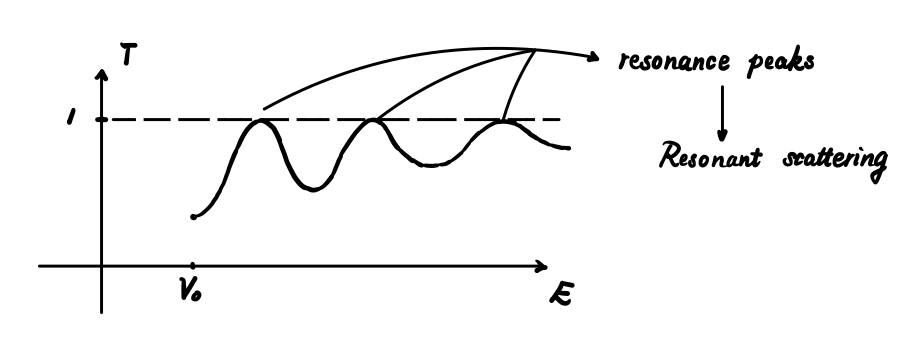
\includegraphics[scale = 1]{square-barrier-transmission.png}
\end{center}
We may use this property to determine the thickness $a$ and potential $V_0$ from fitting this model to experimental data. This allows ``quantum sensing'' of a material. Since the condition for peaks in $T$ is $la = n\pi$, we have
\begin{align*}
    n\pi &= a \cdot \sqrt{\frac{2\mu(E - V_0)}{\hbar^2}} \\
    E - V_0 &= \frac{n^2 \pi^2}{a^2} \cdot \frac{\hbar^2}{2\mu}
\end{align*}
which gives us the energy of a particle in a box of size $a$. The resonant peaks occur where $a$ is a half-integer multiple of the particle's wavelength. And not passing the barrier is the same as wavelength misalignment.

\subsection{Quantum Tunnelling - 量子隧穿}
Similar to the square barrier, the ansatz of quantum tunnelling will be:
$$\psi(x) = \begin{cases}
    Ae^{\imag k x} + Be^{-\imag k x}, & L, k = \sqrt{\frac{2\mu E}{\hbar^2}} \\
    Ce^{b x} + De^{-b x}, & \text{interaction, } b = \sqrt{\frac{2\mu(V_0 - E)}{\hbar^2}} \\
    Fe^{\imag k x}, & R, k = \sqrt{\frac{2\mu E}{\hbar^2}}
\end{cases}$$
From \href{https://en.wikipedia.org/wiki/Quantum_tunnelling}{\textcolor{cyan}{Wikipedia}}, the graphical representation of quantum tunnelling is the following:
\begin{center}
    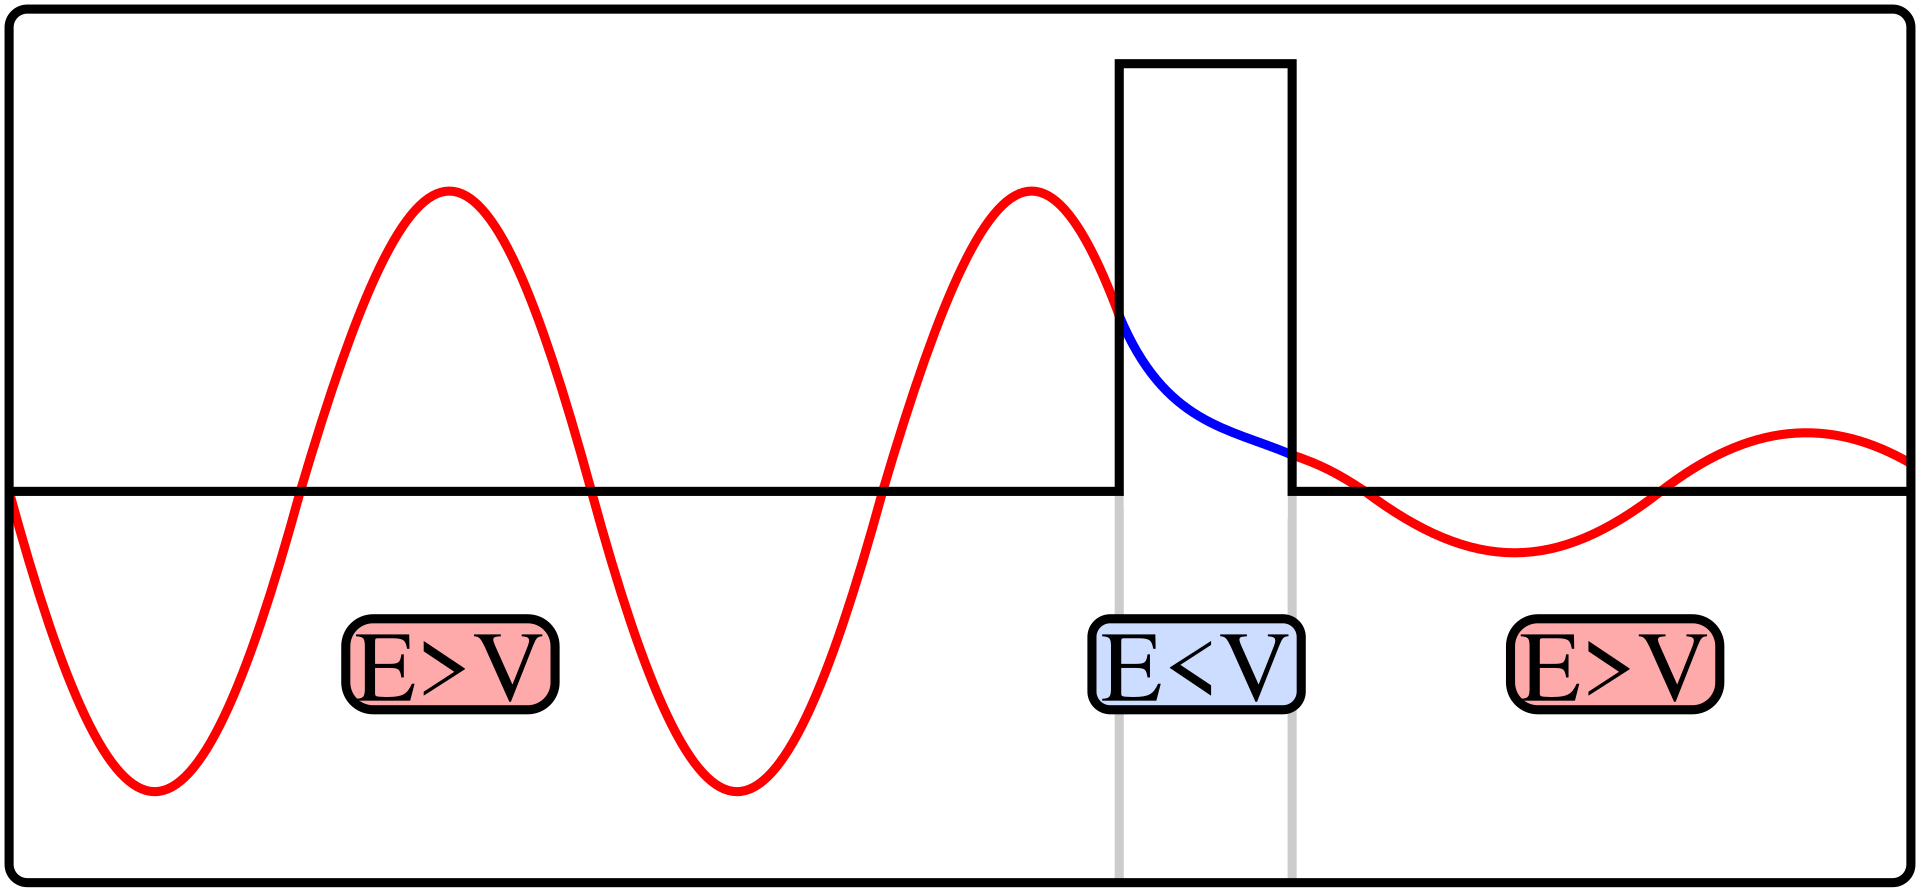
\includegraphics[scale = 0.2]{quantum-tunnelling.png}
\end{center}
That is, there exists a possibility to find the particle on the other side of the box, but the amplitude is drastically dampened.

\newpage
\section{Harmonic Oscillator - 谐振}
Suppose a degree of freedom $x$ (position, angle, current, stress, etc.) is subject to some potential function $V(x)$. We wish to zoom-in and ask what is the effective potential for this degree of freedom close to a stable equilibrium of the potential (local minimum). \\
We assume near $x_0$, we may Taylor expand the potential function to be:
$$V(x) = V(x_0) + V'(x_0)(x - x_0) + \frac{1}{2}V''(x_0)(x-x_0)^2 + \dots$$
Since we are analyzing near a local minimum, we have $V'(x_0) = 0$ and $V''(x_0) > 0$. By ``ignoring'' the smaller terms, we essentially have:
$$V(x) \approx V_0 + \frac{1}{2}V''(x_0)(x-x_0)^2$$
which is a quadratic potential, or a harmonic potential.

\subsection{Classial Harmonic Oscillator - 经典谐振}
A classical harmonic oscillator has the equation of motion:
$$m \cdot \pdv[2]{t} x = -\pdv{V}{x} = -V''(x_0)(x-x_0)$$
This solution to this differential equation is
$$x(t) = A \cos(\omega(t - t_0)) + x_0, \omega = \sqrt{\frac{V''(x_0)}{m}}$$
Some classical examples are springs, the pendulum, molecular vibration, fluctuating fields, LC circuits, and phonons in lattice.

\subsection{Quantum Harmonic Oscillator - 量子谐振}
For a quantum harmonic oscillator, the Hamiltonian is:
$$\hamiltonian = \frac{\opmtm^2}{2\mu} + \frac{1}{2}\mu \omega^2 \oppos^2$$
where we set $V_0 = 0$, $x_0 = 0$, it being time-independent, and we are working in a 1D continuous space. \par
Our goal here is to solve the Schr\"odinger's Equation for $\hamiltonian$, which is by solving the eigenvalue problem $\hamiltonian \ket{n} = E_n \ket{n}$, and find all the stationary states. \par
The Schr\"odinger's Equation is as follows:
$$-\frac{\hbar^2}{2\mu} \pdv[2]{x}\psi_n(x) + \frac{1}{2}\omega^2 x^2 \psi_n(x) = E_n \psi_n(x)$$
This equation can be solved analytically by directly diagonalize $\hamiltonian$, which is an algebraic approach, instead of a direct solution. \par
We start by defining some ``ladder'' operators:
\begin{definition}
    The \uimpt{annihilation operator} is defined to be:
    $$\annih = \sqrt{\frac{\mu \omega}{2\hbar}}\oppos + \imag \frac{1}{\sqrt{2\mu\omega\hbar}}\opmtm$$
    The corresponding \uimpt{creation operator} is the complex adjoint of the annihilation operator, which is:
    $$\creat = \sqrt{\frac{\mu \omega}{2\hbar}}\oppos - \imag \frac{1}{\sqrt{2\mu\omega\hbar}}\opmtm$$
\end{definition}
This means, the position observable and the momentum observable can be expressed in terms of these operators in the following way:
\begin{align*}
    \oppos &= \sqrt{\frac{\hbar}{2\mu\omega}}(\annih + \creat) \\
    \opmtm &= -\imag \sqrt{\frac{\mu \omega \hbar}{2}}(\annih - \creat)
\end{align*}
By utilizing $[\oppos, \opmtm] = \imag \hbar \id$, we have
\begin{lemma}
    The commutator of the annihilation and creation operator is:
    $$[\annih, \creat] = \id$$
\end{lemma}
This lemma can be shown by directly commuting the two operators with the position-momentum commutator being used in the process. \par
By defining such operators, we can then express the Hamiltonian with them, and through substituing $\oppos, \opmtm$ in terms of $\annih, \creat$, we have:
$$\hamiltonian = \hbar \omega (\creat \annih + \frac{1}{2}\id)$$
\begin{definition}
    Define the \uimpt{number operator} $\hat{n}$ to be:
    $$\hat{n} = \creat\annih$$
\end{definition}
It is trivial to see that $[\hamiltonian, \opnum] = 0$, and $\opnum$ is \impt{Hermitian}. That means, it is a conserved quantity for $\hamiltonian$, and if we solve the eigenvalue problem for $\opnum$, we solve the Schr\"odinger's Equation. \par
Let $\ket{n}$ be the eigenvector of $\opnum$, then $\opnum \ket{n} = n \ket{n}$, and so far $n$ is open and unknown. Then, from $[\opnum, \creat] = \creat$ and $[\opnum, \annih] = -\annih$, we have:
\begin{align*}
    \opnum(\creat\ket{n}) &= \creat(\opnum\ket{n}) + \creat\ket{n} \\
    &= \creat(n\ket{n}) + \creat\ket{n} \\
    &= (n+1) \creat\ket{n} \\
    \opnum(\annih\ket{n}) &= (n-1)\annih\ket{n}
\end{align*}
So, $\creat\ket{n}$ is an eigenvector of $\opnum$ with eigenvalue $n+1$; $\annih\ket{n}$ is an eigenvector of $\opnum$ with eigenvalue $n-1$. Since $\opnum$ has a non-degenerate eigenspace, we have $\creat\ket{n} \propto \ket{n+1}$ and $\annih \ket{n} \propto \ket{n-1}$. Assume that $\ket{n}$ are normalized, that is $\braket{n} = 1$ (restricting mathematical solutions to physical solutions), when we define:
$$\ket{\tilde{n+1}} = \creat \ket{n}$$
We have the $\braket{\tilde{n+1}} = n + 1$. By applying the same logic to $\creat \ket{n}$, we have two important properties:
\begin{align*}
    \creat \ket{n} &= \sqrt{n+1}\ket{n+1} \\
    \annih \ket{n} &= \sqrt{n} \ket{n-1}
\end{align*}
We first know:
$$\forall v \in \hilbert, \mel{v}{\opnum}{v} = \mel{v}{\creat\annih}{v} = \braket{av}{av} \ge 0$$
This means $n$ must be non-negative real numbers, as $\ket{n}$ are also part of the Hilbert space. \\
Next, let $k$ be a non-negative integer, we have
$$0 \le \mel{n}{\opnum^k}{n} = \mel{n}{(\creat)^k(\annih)^k}{n}$$
This further derives to:
\begin{align*}
    \mel{n}{(\creat)^k(\annih)^k}{n} &= \mel{n-1}{(\creat)^{k-1}(\annih)^{k-1}}{n-1} \cdot \sqrt{n} \cdot \sqrt{n} \\
    &= \braket{n-k} \cdot n \cdot (n-1) \cdot \dots \cdot (n-k+1)
\end{align*}
This means, $n$ must be a non-negative integer, otherwise, there exists a $k$ such that the series product will be negative. \par
We find for the Hamiltonian $\hamiltonian = \hbar \omega (\creat \annih + \frac{1}{2}\id)$ has eigenvalues $\{\frac{1}{2}\hbar\omega, \frac{3}{2}\hbar\omega, \frac{5}{2}\hbar\omega, \dots\}$ for normalizable eigenvectors. \\
Now we need to construct the corresponding eigenstates. We first start with $\ket{0}$, we know $\annih \ket{n} = \sqrt{n}\ket{n-1}$, so $\annih\ket{0} = \vec{0}$. The annihilation operator on the position wavefunction is:
$$\annih: \psi(x) \mapsto \sqrt{\frac{\mu \omega}{2\hbar}} \cdot x \cdot \psi(x) + \imag \frac{1}{\sqrt{2\hbar \mu \omega}} (-\imag \hbar)\pdv{x}\psi(x)$$
Therefore, the differential equation for $\psi_0(x)$ (the position wavefunction of $\ket{0}$) is:
\begin{align*}
    \frac{1}{\sqrt{2\hbar}}(\sqrt{\mu\omega}x + \frac{\hbar}{\sqrt{\mu\omega}}\pdv{x})\psi_0(x) &= 0 \\
    \psi_0(x) &= \frac{1}{\sqrt[4]{\frac{\hbar\pi}{\mu\omega}}} \cdot \exp(-x^2 \cdot \frac{\mu\omega}{2\hbar})
\end{align*}
For other $n \in \N$, we start with $\creat\ket{n} = \sqrt{n+1}\ket{n+1}$, then this gives:
$$\creat\ket{0} = \sqrt{n!}\ket{n}$$
which means the position wavefunction of $\ket{n}$ is essentially:
$$\psi_n(x) = \frac{1}{\sqrt{n!}} (\creat)^n \psi_0(x) = \frac{1}{\sqrt{n!}} (\sqrt{\frac{\mu\omega}{2\hbar}}x - \imag \frac{-\imag \hbar}{\sqrt{2\hbar\mu\omega}}\pdv{x})^n \psi_0(x)$$
This eventually solves to:
$$\psi_n(x) = \frac{1}{n! \cdot (\frac{2\hbar}{\mu\omega})^n\sqrt{\frac{\hbar\pi}{\mu\omega}}} \cdot H_n(x) \cdot \exp(-x^2 \cdot \frac{\mu\omega}{2\hbar})$$
where $H_n(x)$ are the \impt{Hermite polynomials}.
\begin{center}
    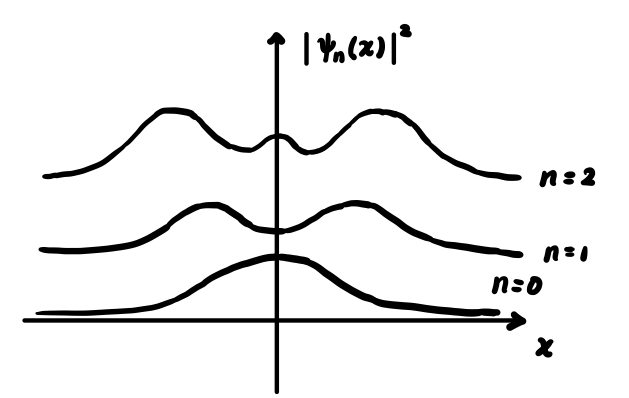
\includegraphics[scale = 1]{ho-prob-dist.png}
\end{center}
Note that the normalizability condition for $\ket{n}$ led to a discrete energy spectrum. The minimal energy $E_0 = \frac{1}{2}\hbar\omega$, meaning that the harmonic oscillator is never at rest, this is the ``zero-point'' energy. \\
It is also possible to discuss the ``classical limits''. This is considering the high energy eigenstates where $n$ is much larger than $1$. It thus has the probability distribution of:
\begin{center}
    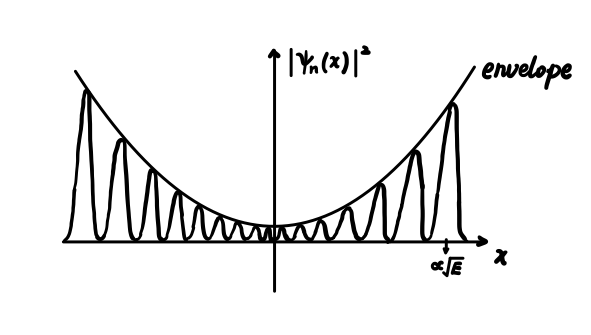
\includegraphics[scale = 1]{ho-high-energy.png}
\end{center}
The probability distribution approaches the classical probability distribution emerged over time, up to fluctuations, $n$ is the number of fluctuations. This ``envelope'' is the probability distribution in $x$ averaged over time. \\
Take a pendulum as an example, where the $x$ of interest is the angle. If we look at the angle at random times, the time-averaged ``angle'' will have an angle density for angle $p(x)$. The pendulum stays longer at the maximum height, and stays shorter at the minimum height. 
\begin{center}
    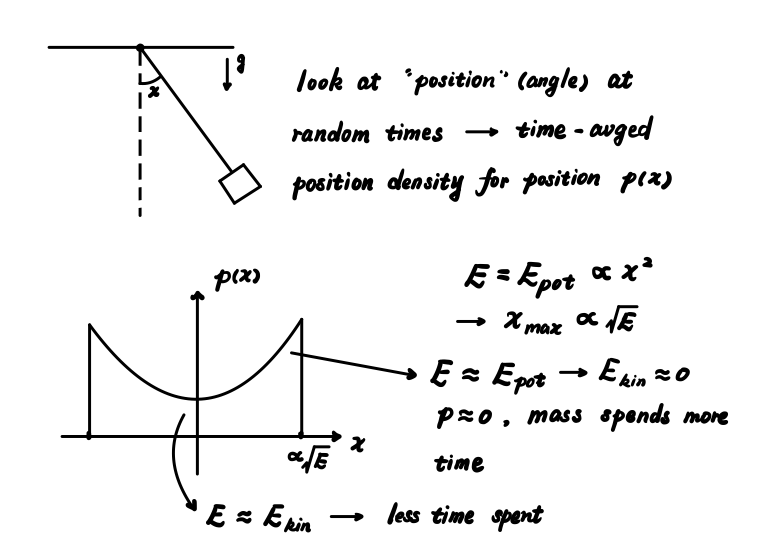
\includegraphics[scale = 1]{ho-classical-lim.png}
\end{center}
Be careful that the energy eigenstates are stationary, so $\expval{\oppos}_t, \expval{\opmtm}_t$ remains constant, there is no oscillations observable from these two observables.
\begin{definition}
    \uimpt{Coherent states} are classically oscillating quantum states, typically denoted by $\ket{\alpha}, \alpha \in \C$
\end{definition}
If we plot the position observable and momentum observable expectation values, we have:
\begin{center}
    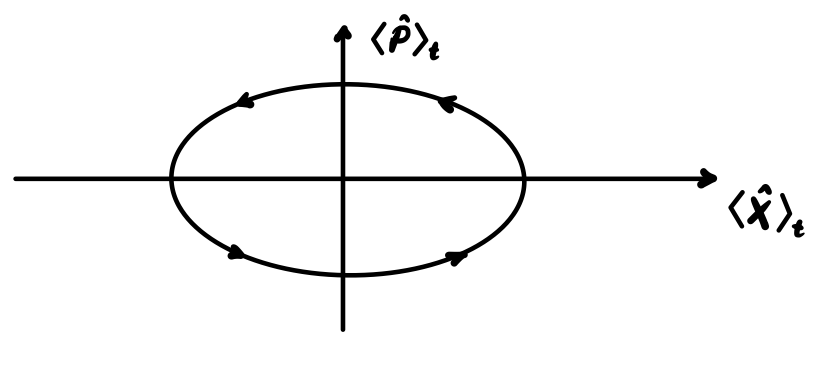
\includegraphics[scale = 1]{coherent-state.png}
\end{center}
It is going to oscillate around with uniform velocity in the ellipse, and we can map the $x$-component to $\sin$ and the $y$-component to $\cos$. A laser field can be such an example.

\newpage
\section{Uncertainty Relations - 不确定性}
We know the relationship between the position and momentum basis through their inner product, 
$$\begin{matrix}
    \ket{x} \\
    \ket{p}
\end{matrix} = \frac{1}{\sqrt{2\pi\hbar}} \intR \exp(\mp \frac{\imag p x}{\hbar}) \begin{matrix}
    \ket{p} \\ \ket{x}
\end{matrix} \dd \begin{matrix}
    p \\ x
\end{matrix}$$
Consider $\Prob{p}_{\ketx}$, notice that this probability density is uniform, as $\abs{\frac{1}{\sqrt{2\pi\hbar}}\exp(\mp \frac{\imag p x}{\hbar})}^2$ is a constant and independent of $x$ or $p$. So, if we have complete certainty in $\ket{x}$, we have \impt{complete uncertainty} about $\ket{p}$. This relation is the consequence of $[\oppos, \opmtm] = \imag \hbar$.
\begin{theorem}
    Let $\hilbert$ be an arbitrary quantum system, and consider $\ketpsi \in \hilbert$ with $A = \conjt{A}, B = \conjt{B}$. Then, we first have:
    $$(\Delta A)^2 = \expval{A^2}{\psi} - (\expval{A}{\psi})^2$$
    $$(\Delta B)^2 = \expval{B^2}{\psi} - (\expval{B}{\psi})^2$$
    then the \uimpt{Robertson Uncertainty Principle} says that
    $$\forall \ketpsi \in \hilbert, \Delta A \Delta B \ge \frac{1}{2}\abs{\expval{[A, B]}{\psi}}$$
\end{theorem}
From the Robertson Uncertainty Principle, we substitute $A, B$ with $\oppos, \opmtm$, we thus have,
\begin{theorem}
    The \uimpt{Heisenberg Uncertainty Principle} says that
    $$\Delta \oppos \Delta \opmtm \ge \frac{1}{2}\abs{\expval{[\oppos, \opmtm]}{\psi}} = \frac{\hbar}{2}$$
\end{theorem}
The Robertson Uncertainty Principle is proven through Cauchy-Schwarz Inequality, where we take the lower bound to be the absolute value of the imaginary part of the inner product (for tighter bounds, we can use the real part of the inner product). \par
Consider the following examples,
\begin{quote}
    1. Gaussian wavepackets:
    $$\psi(x) = \frac{1}{\sqrt[4]{2\pi\sigma^2}}\exp(-\frac{(x-x_0)^2}{4\sigma^2})\exp(\imag k x) \to (\Delta X)^2 = \sigma^2$$
    $$\tilde{\psi}(p) = \sqrt[4]{\frac{2\sigma^2}{\pi \hbar^2}}\exp(-\frac{(p - \hbar k)^2}{4\hbar^2 / 4\sigma^2})\exp(-\frac{\imag x_0 (p-\hbar k)}{\hbar}) \to (\Delta P)^2 = \frac{\hbar^2}{4\sigma^2}$$
    From this, we have $\Delta X \Delta P = \frac{\hbar}{2}$, which is exactly the minimum joint uncertainty on $X$ and $P$. \\
    2. Spin Measurements / Qubit Measurements: we first have $\hilbert = \Span{\ket{0}, \ket{1}}$, then with the operators $\hat{S}_{x, y, z} = \frac{\hbar}{2}X, Y, Z$. We know $[X, Z] = -2\imag Y$, then $[\hat{S}_x, \hat{S}_z] = -\imag\hbar \hat{S}_y$. Then the uncertainty is:
    $$\Delta \hat{S}_x \Delta \hat{S}_z \ge \frac{1}{2}\abs{\expval{\hat{S}_y}{\psi}}$$
    which is \impt{state dependent}. If $\ketpsi = \ket{+\imag}$, the uncertainty will be $\ge (\frac{\hbar}{2})^2$; if $\ketpsi = \ket{1}$, the uncertainty will be $\ge 0$ (trivial).
\end{quote}
The Robertson Uncertainty Principle only implies the trivial case, that is, $\Delta A \Delta B \ge 0$, when $[A, B] = 0$ ($A,B$ commute) or $[A, B] \ne 0$ but the commutator is orthogonal to $\ketpsi$. \\
The lower bound is state-independent when the commutator is proportional to $\id$. The bound is also state-independent for general states only if it is an \impt{infinite-dimensional} space.

\newpage
\section{Quantum Spins - 粒子自旋}
We start by motivating \impt{``spin''} as a finite-dimensional degree of freedom in quantum mechanics. \\
We have the following observations:
\begin{quote}
    1. Consider the spectral analysis of quantum systems, with Hamiltonians invariant on rotations (rotationally invariant), and the rotation is $R \in SO(3)$, we see a spectrum of energy levels $\{E_i\}$. As soon as we start working with a Hamiltonian that is \impt{not rotationally invariant}, then each of the previously observed energy levels $E_i$ will be split into $2j+1$ levels (finitely many), where $j \in \{0, \frac{1}{2}, 1, \frac{3}{2}, \dots\}$. This is in the premise of:
    $$SO(3) = \{R \in \R^{3 \times 3} \mid R^{\top}R = RR^{\top} = \id, \det(R) = 1\}$$
    This represents all rotations in 3D space. $S$ means ``special'', $O$ means ``orthogonal''. \\
    2. For Stern-Gerlach, without the magnet, the particle shot out with energy $E$ would only have one energy level, with rotational invariance around the beam axis. However, with a magnet, the Hamiltonian is no longer rotationally invariant around the beam axis, so the energy level splits into $2j+1, j=\frac{1}{2}$ levels.
\end{quote}
The intermediate conclusion from these observations that:
\begin{quote}
    1. Depending on the particle, there exists an additional finite-dimensional degree of freedom that needs to be described. \\
    2. It becomes visible (physically relevant) if the setting is not symmetric under rotations $\iff$ if the setting is rotationally invariant, this degree of freedom is a \impt{conserved quantity}. \\
    3. The conserved quantity associated with rotational invariance (N\"other's theorem) is \impt{angular momentum} ($\hat{\vec{L}} = \hat{\oppos} \times \hat{\opmtm}$). So ``spin'' is ``some sort of'' angular momentum, and its unit is equal to $[\vec{L}] = [\hbar]$. \\
    4. In order to investigate spin, we must investigate how quantum systems and states transform under 3D rotations.
\end{quote}
It is important to distinguish between physical settings and their corresponding mathematical descriptions. In this case, a transformation in the physical space in mathematical representation is unitary representations of groups on $\hilbert$.
\begin{definition}
    Let $G$ be a group and $\hilbert$ be a Hilbert space. \uimpt{A unitary representation} of $G$ on $\hilbert$ is the map
    $$\mathfrak{U}: G \to \text{GeneralLinearOperator}(\hilbert) := \{A:\hilbert \to \hilbert \mid A \text{ is linear and invertible}\}$$
    such that
    \begin{quote}
        1. $\mathfrak{U}(g)$ is a linear operator on $\hilbert$. (Being well-defined) \\
        2. $\mathfrak{U}(g_1g_2) = \mathfrak{U}(g_1)\mathfrak{U}(g_2)$. (Homomorphism) \\
        3. $\conjt{\mathfrak{U}(g)} = \mathfrak{U}(g)^{-1}$. (Unitary)
    \end{quote}
\end{definition}
Take $G = SO(3)$ and $\hilbert = \hilbert_{x_1} \otimes \hilbert_{x_2} \otimes \hilbert_{x_3}$ as an example. Let $\ketpsi \in \hilbert$, with position wavefunction $\psi(\vec{x})$, a trivial representation would be $\forall R \in SO(3), \urep(R) = \id$. Then, in general,
\begin{align*}
    \urep: SO(3) &\to GL(\hilbert) \text{ with } \psi(\vec{x}) \mapsto \psi(R^{-1}\vec{x}) \\
    R &\mapsto \urep(R)
\end{align*}
is a unitary representation of $SO(3)$ on $\hilbert$. \\
We are only interested in the representations that act non-trivially on the full $\hilbert$ space. These representations are considered \impt{irreducible}. Turns out, there is exactly $1$ finite-dimensional irreducible representation for each dimension. These irreducible unitary representations of $SO(3)$ in finite dimensions are the following:
\begin{align*}
    \C^1 \cong \mathcal{D}_0 &: \urep(R) = \id, \text{ scalar, spin-}0 \\
    \C^2 \cong \mathcal{D}_\frac{1}{2} &: \urep(R) = \exp(-\frac{\imag \theta}{2}(e_1X + e_2Y + e_3Z)), \text{ spinor, spin-}\frac{1}{2} \\
    \C^3 \cong \mathcal{D}_1 &: \urep(R) = R, \text{ vector, spin-}1 \\
    \C^4 \cong \mathcal{D}_\frac{3}{2} &: \text{ spin-}\frac{3}{2} \\
    \C^5 \cong \mathcal{D}_2 &: \text{ tensor, spin-}2
\end{align*}
The $\mathcal{D}$ is the representation. \\
It concludes that the Hilbert space of spin-$j$ in 3D space is:
$$\hamiltonian_{\text{tot}} = \hilbert_{x_1} \otimes \hilbert_{x_2} \otimes \hilbert_{x_3} \otimes \mathcal{D}_j$$
and under $R \in SO(3)$ the transformation is:
$$\psi(\vec{x}) \cdot \phi \mapsto \psi(R^{-1}\vec{x}) \cdot \urep(R)\phi$$
Scalars, vectors, and tensors are odd-dimensional representation of $SO(3)$ (classical), while spin-$\frac{1}{2}$ and spin-$\frac{3}{2}$ are representations only of $SU(2)$. $SO(3)$ and $SU(2)$ differ by:
\begin{quote}
    1. Physical quantities related to direction are described by vectors, whose rotations are described by rotation matrices of $SO(3)$. \\
    2. Some quantities like spin are described by spinors, whose rotations are described by rotation matrices of $SU(2)$.
\end{quote}
Here,
$$SU(2) = \{\opuni \in \C^{2 \times 2} \mid \conjt{\opuni}\opuni = \opuni\conjt{\opuni} = \id, \det\opuni = 1\}$$
To explain the transformation further, take $\urep_{\frac{1}{2}}(R)$ specifically, $R$ is a rotation around $\vec{e}$ and $\abs{\vec{e}} = 1$, about some angle $\theta$.
\begin{definition}
    Spin-$j$ is a $2j+1$ degrees of freedom with unit of angular momentum $[\hbar]$ and corresponds to an observable:
    $$\hat{\vec{S}} = \begin{pmatrix}
        \hat{S}_x \\ \hat{S}_y \\ \hat{S}_z
    \end{pmatrix}$$
\end{definition}
For spin-$\frac{1}{2}$, the observable is specifically:
$$\hat{\vec{S}} = \frac{\hbar}{2}\begin{pmatrix}
    X \\ Y \\ Z
\end{pmatrix}$$
Some spin-$j$ particles have an associated magnetic moment. First consider a general angular momentum graph:
\begin{center}
    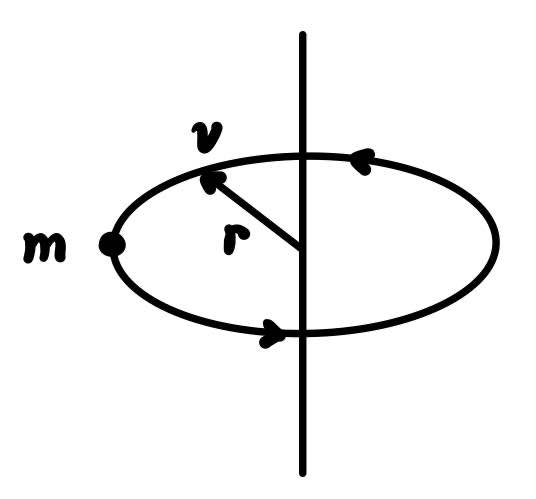
\includegraphics[scale = 0.25]{spin-angular-mtm.jpg}
\end{center}
We have $\abs{\vec{L}} = \abs{\vec{x} \times \vec{p}} = r \cdot m \cdot v$. If charged, it will behave as a magnetic moment $\vec{\mu}$:
$$\vec{\mu} = -\frac{g_s \cdot \mu_B}{\hbar} \cdot \hat{\vec{S}}$$
where $g_s$ is the gyromagnetic factor (different dependent on the particle), and $\mu_B$ is the Bohr magneton $\frac{e \cdot \hbar}{2m_e} \approx 9.3 \text{ J/T}$.

\subsection{Bosons and Fermions - 玻色子和费米子}
\begin{definition}
    Particles with integer spin ($j = 0, 1, 2, \dots$) are \uimpt{bosons}. \\
    Particles with half-integer spin ($j = \frac{1}{2}, \frac{3}{2}, \dots$) are \uimpt{fermions}.
\end{definition}
Some examples of bosons are: photons (spin-$1$), $\Omega$ and $Z$ bosons, Higgs bosons, gluons; some examples of fermions are: photons, neutrons, electrons, quarks, and $\nu$.
\begin{theorem}
    \uimpt{Pauli Exclusion Principle} states that no $2$ fermions in a quantum system can have the same quantum state.
\end{theorem}

\newpage
\section{Density Operator Formalism - 密度运算符}
When using quantum systems for \impt{processing information} (i.e. ``doing quantum information processing''), it is necessary to model \impt{missing, incomplete, subjective knowledge} about a state in a quantum system. Some examples are quantum key exchange (imperfect state preparation), errors during a quantum computation (imperfect measurements), and inaccurate model of a Hamiltonian. \par
Classically, if we have perfect knowledge about a state of a system, say an $n$-bit string, the state is a specific bit string $\vec{b} \in \{0, 1\}^n$. However, with imperfect or subjective knowledge, a ``state'' is a probability distribution over $\{0, 1\}^n$. The probability map would be:
$$\Prob{\vec{b}}: \vec{b} \in \{0, 1\}^n \to [0,1]$$
where we satisfy $\sum \Prob{\vec{b}} = 1$ and $\Prob{\vec{b}} \ge 0$. \par
In a quantum formalism, a state is a normalized vector $\ketpsi \in \hilbert$. The corresponding imperfect representation would be \impt{density operators}. \par
Suppose a quantum system associated with $\hilbert$ is prepared according to:
\begin{quote}
    1. Generate a number $i \in \{1, \dots, n\}$ with probability $\text{Pr}_i$, where $\text{Pr} \ge 0$ and $\displaystyle \Sum{i = 1}{n} \text{Pr}_i = 1$. \\
    2. Prepare the quantum state $\ket{\psi_i} \in \hilbert$, where $\{\ket{\psi_i}_{i = 1}^n\}$ is an arbitrary set of quantum states.
\end{quote}
We now wish to know how we can efficiently describe this ``state'', if we do not know $i$. In words, we can say: state $\ket{\psi_i}$ with probability $\text{Pr}_i$; or mathematically, as \impt{probability mixtures}: $\{(\text{Pr}_i, \ket{\psi_i})\}_{i=1}^n$. \par
We can find a more efficient mathematical object that captures \impt{all relevant information} of a probability mixture, where all relevant information is \impt{the probability of measurement outcomes}. We then calculate the outcome probability of a measurement with respect to projection operators $\{\Pi_x\}_x$:
\begin{align*}
    \Prob{x: \{(\text{Pr}_i, \ket{\psi_i})\}} &= \Sum{i = 1}{n} \Prob{\ket{\psi_i}} \times \Prob{x \mid \ket{\psi_i}} \\
    &= \Sum{i=1}{n} \text{Pr}_i \ev{\Pi_x}{\psi_i} \\
    &= \Sum{i=1}{n} \text{Pr}_i \tr(\Pi_x \dyad{\psi_i}) \\
    &= \tr(\Pi_x \cdot \Sum{i=1}{n} \text{Pr}_i \dyad{\psi_i})
\end{align*}
This result comes from the property of the trace. Consider the orthonormal basis of $\Pi_x \dyad{\psi_i}$ to be $\{\ket{\phi_k}\}_{k=1}^d$, we choose $\ket{\phi_1} = \ket{\psi_i}$ and complete the basis accordingly, we then have:
\begin{align*}
    \tr(\Pi_x \dyad{\psi_i}) &= \Sum{k=1}{d} \mel{\phi_k}{\Pi_x}{\psi_i}\braket{\psi_i}{\phi_k} \\
    &= \mel{\phi_1}{\Pi_x}{\psi_i} \\
    &= \ev{\Pi_x}{\psi_i}
\end{align*}
\begin{definition}
    Given a Hilbert space $\hilbert$, and prepare a number of states $\{\ket{\psi_i}\}_{i=1}^n$ with each state having the probability of $p_i$, then, the \uimpt{density operator} that represent this ``state'' is
    $$\rho = \Sum{i=1}{n} p_i \dyad{\psi_i}$$
\end{definition}
Note that the density operator is a convex linear combination of projectors, hence $\rho: \hilbert \to \hilbert$ is a linear operator. Some properties of the density operator include:
\begin{quote}
    1. $\rho$ is Hermitian \\
    2. $\rho \ge 0$ is semi-definite: $\ev{\rho}{\phi} = \sum p_i \braket{\phi}{\psi_i}\braket{\psi_i}{\phi} = \sum p_i \abs{\braket{\phi}{\psi_i}}^2 \ge 0$. \\
    3. $\tr(\rho) = 1$: $\tr(\Sumi{i}p_i \dyad{\psi_i}) = \Sumi{i}p_i \tr(\dyad{\psi_i}) = \Sumi{i}p_i = 1 $
\end{quote}
\begin{theorem}
    Any Hermitian, positive semi-definite, unit trace operator $\sigma$ can be written as:
    $$\sigma = \Sumi{i} q_i \dyad{\phi_i}$$
    where $\{q_i\} \subseteq \R$ and $\{\ket{\phi_i}\}$ is an orthonormal basis. \\
    $\sigma$ corresponds to (can be interpreted as) the probability mixture:
    $$\{(q_i, \ket{\phi_i})\}_i$$
    This is not unique.
\end{theorem}
This is essentially the spectral decomposition of a density operator. \\
The set of density operators (a.k.a ``quantum states'') of a system associated to $\hilbert$ is:
$$\mathcal{S}(\hilbert) = \{\rho \text{ is a linear operator on }\hilbert \mid \rho \ge 0, \conjt{\rho} = \rho, \tr(\rho) = 1\}$$
For density operators, $\rho \in \mathcal{S}(\hilbert)$ does not specify a unique probability mixture, which inherently tells us that probability mixtures are redundant.
\begin{definition}
    The density operator $\rho$ is \uimpt{pure}, if there exists $\ketphi \in \hilbert$, $\rho = \dyad{\phi}$. This uniquely defines a probability mixture. If $\rho$ is not pure, it is \uimpt{mixed}.
\end{definition}
A mixture of mixed states is also a mixed state. That is, consider a probability mixture $\{(q_i, \sigma_i)\}$, where $\sigma_i \in \mathcal{S}(\hilbert)$, the corresponding density operator:
$$\rho = \sum q_i \cdot \sigma_i$$
is also a mixed state. 
\begin{definition}
    $\rho$ is \uimpt{maximally mixed} if $\rho = \frac{\id}{\dim(\hilbert)}$
\end{definition}
This is essentially a uniform distribution in a classical sense. \\
Notice that for composite system $\hilbert_A \otimes \hilbert_B$, the set of density operators are defined:
$$\mathcal{S}(\hilbert_A \otimes \hilbert_B) = \{\rho \text{ is a linear operator on }\hilbert \mid \rho \ge 0, \conjt{\rho} = \rho, \tr(\rho) = 1\}$$
$$\mathcal{S}(\hilbert_A \otimes \hilbert_B) \ne \mathcal{S}(\hilbert_A) \otimes \mathcal{S}(\hilbert_B)$$
as $\mathcal{S}$ is not a linear space. \\
To compare the vector formalism and the density operator formalism, refer to the following table:
\begin{center}
    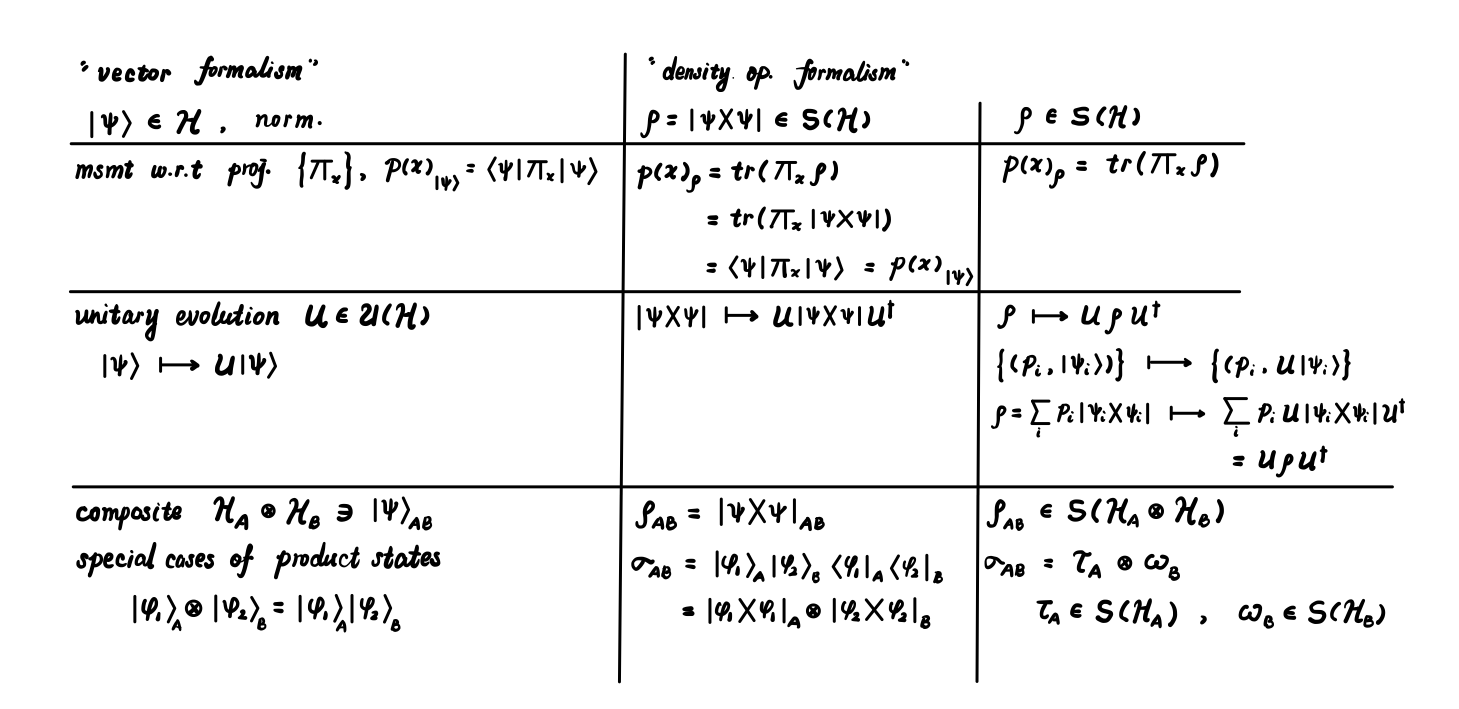
\includegraphics[scale = 0.625]{vec-rho.png}
\end{center}

\subsection{Partial Trace}
Consider a bipartite state $\rho_{AB} \in \mathcal{S}(\hilbert_A \otimes \hilbert_B)$, we want to find a way (an operation) to ``reduce'' $\rho_{AB}$ to a ``local state'', say $\rho_A \in \mathcal{S}(\hilbert_A)$, such that $\rho_A$ captures all physical properties of the $A$ system. Mathematically, this is finding an operation that maps $\rho_{AB} \mapsto \rho_A$ such that all projective measurements on $A$ $\{\Pi_x\}$:
$$\Prob{x}_{\rho_{AB}} = \tr((\Pi_x \otimes \id)\rho_{AB}) = \tr(\Pi_x \rho_A) = \Prob{x}_{\rho_A}$$
Recall that any linear operator $M_{AB}$ on $\hilbert_A \otimes \hilbert_B$ can be written as:
$$M_{AB} = \Sumi{k} S_k \otimes T_k$$
Then,
\begin{definition}
    The \uimpt{partial trace} over $B$ when $\hilbert = \hilbert_A \otimes \hilbert_B$ is map where:
    \begin{align*}
        \tr_B: \{\text{linear operator on the composite system}\} &\to \{\text{linear operator on }\hilbert_A\} \\
        M_{AB} = \Sumi{k} S_k \otimes T_k &\mapsto \Sumi{k} S_k \cdot \tr(T_k)
    \end{align*}
\end{definition}
If $\rho_{AB} \in \mathcal{S}(\hilbert_A \otimes \hilbert_B)$, then $\rho_A = \tr_B(\rho_{AB}) \in \mathcal{S}(\hilbert_A)$ is also a vaild density operator. The partial trace is essentially a map that maps an \impt{endomorphism of the composite system} to an \impt{endomorphism of the local system}. The local trace $\rho_A := \tr_B(\rho_{AB})$ is called the marginal (compare to the marginals of probability distributions)/reduced/local state. Applying the partial trace $\tr_B$, we say ``\impt{we trace out B}''. Different global states $\rho_{AB}$ can lead to the same local state. Marginals of pure states are not necessarily pure. \\
Recall that our goal was to find the ``reduction'', and we claim the partial trace does the job. To start with, consider these two elementary properties of the partial trace:
\begin{quote}
    1. $\tr(M_{AB}) = \tr(\tr_B(M_{AB}))$. \\
    2. $\tr_B((N_A \otimes \id_B)M_{AB}) = N_A \tr_B(M_{AB})$
\end{quote}
Then, 
\begin{align*}
    \tr((\Pi_x \otimes \id)\rho_{AB}) &= \tr(\tr_B((\Pi_x \otimes \id)\rho_{AB})) \\
    &= \tr(\Pi_x \tr_B(\rho_{AB})) \\
    &= \tr(\Pi_x \rho_A)
\end{align*}
This is the unique operation that satisfies this relation for all states $\rho_{AB}$ and all local measurements $\{\Pi_x\}_x$. Thus, we can consider a commutative diagram that relate the composite system and the local system by considering a local unitary evolution:
\begin{center}
    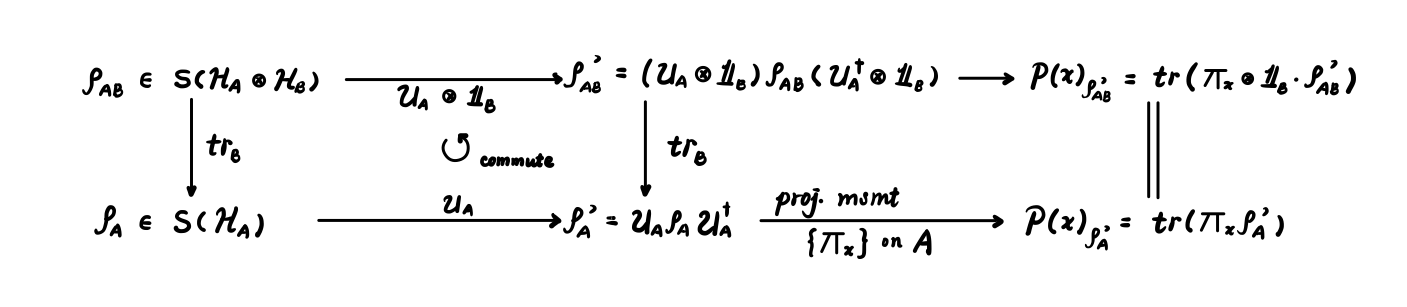
\includegraphics[scale = 0.625]{partial-trace.png}
\end{center}
Now, we are able to reduce the composite system to a local system, we wish to know whether or not we can go the other way round. It is already known that the same local state can map to non-unique composite systems.
\begin{definition}
    Let $\rho_A \in \mathcal{S}(\hilbert_A)$, then a state $\rho_{AB} \in \mathcal{S}(\hilbert_A \otimes \hilbert_B)$ on a bigger and composite $\hilbert$ is called the \uimpt{extension} of $\rho_A$ if
    $$\tr_B(\rho_{AB}) = \rho_A$$
    $\rho_{AB}$ is considered to be the \uimpt{purification} of $\rho_A$ and $B$ is the \uimpt{purifying system} if $\rho_{AB} = \dyad{\phi}_{AB}$ is a \uimpt{pure extension}.
\end{definition}
In fact, $\forall \rho_A \in \mathcal{S}(\hilbert_A)$, $\exists \hilbert_B, \ketpsi_{AB} \in \hilbert_A \otimes \hilbert_B$, such that $\tr_B(\dyad{\psi}_AB) = \rho_A$. This means, \impt{every quantum state can be purified}. Hence, at the cost of working in a larger $\hilbert$, one can always work with pure states. \\
Except for the inefficiency to model ``everything'' (laser interacting with trapped ions) and the impossibility to model ``everything'' (microwave radiation interacting with trapped ions) being reasons that we don't work with pure states only, the other important reason is that we simply can ( through density operators as a formalism).

\subsection{Schr\"odinger's Equation for Density Operators - 密度运算符的薛定谔方程}
We are already familiar with the fact that:
$$\ket{\psi(t)} = \opuni(t)\ket{\psi(0)} = \exp(-\frac{\imag \hamiltonian t}{\hbar}) \ket{\psi(0)}$$
So for $\rho(0) \in \mathcal{S}(\hilbert)$, we first have:
\begin{align*}
    \rho(t) &= \exp(-\frac{\imag \hamiltonian t}{\hbar}) \rho(0) \conjt{\exp(-\frac{\imag \hamiltonian t}{\hbar})} \\
    &= \exp(-\frac{\imag \hamiltonian t}{\hbar}) \rho(0) \exp(+\frac{\imag \hamiltonian t}{\hbar})
\end{align*}
By taking the time derivative, we have:
\begin{align*}
    \pdv{t}\rho(t) &= \pdv{t}\exp(-\frac{\imag \hamiltonian t}{\hbar}) \rho(0) \exp(+\frac{\imag \hamiltonian t}{\hbar}) + \exp(-\frac{\imag \hamiltonian t}{\hbar}) \rho(0) \pdv{t} \exp(+\frac{\imag \hamiltonian t}{\hbar}) \\
    &= (-\frac{\imag \hamiltonian}{\hbar})\rho(t) + \rho(t)(+\frac{\imag \hamiltonian}{\hbar}) \\
    &= -\frac{\imag}{\hbar} [\hamiltonian, \rho(t)]
\end{align*}

\subsection{Expectation Value of Observables in Density Operator Formalism - 基于密度运算符的可观测量的期望值}
For $\ketpsi \in \hilbert$, $\expval{\mathcal{O}}_\psi = \ev{\mathcal{O}}{\psi} = \tr(\mathcal{O}\dyad{\psi})$. Then, it is trivial to see:
$$\forall \rho \in \mathcal{S}(\hilbert), \expval{\mathcal{O}}_\rho = \tr(\mathcal{O}\rho)$$
This is the result of $\mathcal{O} = \sum x \Pi_x$ and the probability of measuring outcome $x$ in state $\ketpsi$ is $\Prob{x}_\psi = \ev{\Pi_x}{\psi}$.
\begin{align*}
    \expval{\mathcal{O}}_\psi &= \sum x \cdot \Prob{x}_\psi \\
    &= \sum x \cdot \ev{\Pi_x}{\psi} \\
    &= \ev{\sum x \cdot \Pi_x}{\psi} \\
    &= \ev{\mathcal{O}}{\psi}
\end{align*}
Furthermore, for $\rho \in \mathcal{S}(\hilbert)$, the probability of measuring outcome $x$ is $\Prob{x}_\rho = \tr(\Pi_x \rho)$, which gives:
\begin{align*}
    \expval{\mathcal{O}}_\rho &= \sum x \cdot \tr(\Pi_x \rho) \\
    &= \tr(\sum x \cdot \Pi_x \rho) \\
    &= \tr(\mathcal{O}\rho)
\end{align*}

\newpage
\section{Additional Topics - 额外主题}
\subsection{Introduction to Quantum Circuits and Quantum Computing - 量子电路和量子计算初探}
Consider an $n$-qubit system with $\hilbert = (\C^2)^{\otimes n} = \C^{2^n}$. A quantum circuit with $n$ qubits can be the following:
\begin{center}
    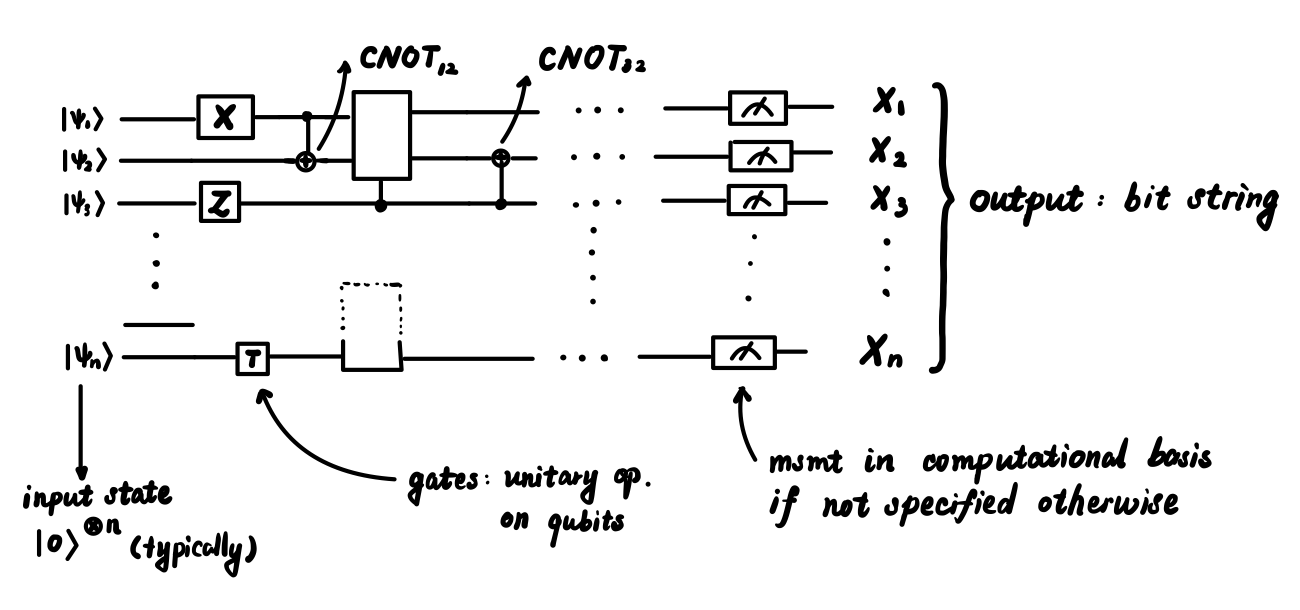
\includegraphics[scale = 0.6]{qcircuit.png}
\end{center}
If we want to measure in a different basis, say the columns of a unitary operator $V$, then one can apply $\conjt{V}$ before the measuring in the computational basis instead. \\
The final measurement give one bitstring per run of the circuit, and good quantum algorithms only need a few runs and results. \\
Discrete gates are typically implemented by turning on and off interactions (lasers, microwave pulses, bringing qubits closer to each other through Coulomb force). Take Pauli-X gate as an example, the Hamiltonian is $H_{\text{int}} = \alpha X$, which gives the unitary propagator to be:
$$\opuni(t) = \exp(-\frac{\imag \alpha X t}{\hbar}) = \cos(\frac{\omega t}{2})\id - \imag \sin(\frac{\omega t}{2})X$$
where $\omega = \frac{\alpha}{\hbar}$. If the interaction acts for $\Delta t = \frac{\pi}{\omega} = \frac{\pi \cdot \hbar}{\alpha}$, then, $\opuni(\Delta t) = (-\imag)X$. \par
Like a classical circuit, the quantum gates play an important role. Consider the controlled gates, an example is the CNOT gate:
\begin{align*}
    \text{CNOT}: \ket{00} &\mapsto \ket{00} \\\
    \ket{01} &\mapsto \ket{01} \\
    \ket{10} &\mapsto \ket{11} \\
    \ket{11} &\mapsto \ket{10}
\end{align*}
A general controlled-$\opuni$ gate would be:
\begin{align*}
    \text{C-}\opuni: \ket{00} &\mapsto \ket{00} \\\
    \ket{01} &\mapsto \ket{01} \\
    \ket{10} &\mapsto \ket{1} \otimes \opuni\ket{0} \\
    \ket{11} &\mapsto \ket{1} \otimes \opuni\ket{1}
\end{align*}
We further wish to know what total unitaries can be implemented on quantum circuits (a unitary that acts on all $n$ qubits). With a universal set of elementary gates, any $\opuni_{\text{tot}} \in \opuni((\C^2)^{\otimes n})$ can be implemented. In \impt{classical computation}, a universal set of gates is the $\{\text{NAND}\}$, that is, if the NAND gate is implemented, any logical operators can be implemented. In quantum computation, some known universal sets are:
\begin{quote}
    1. $\{T, H, \text{CNOT}\}$, where $H$ is the Hadamard, and
    $$T = \begin{pmatrix}
        1 & 0 \\ 0 & \exp(\frac{\imag \pi}{4})
    \end{pmatrix}$$
    This set can approximate any $\opuni_{\text{tot}}$ \impt{up to arbitrary precision}. \\
    2. $\{H, \text{Toffoli}\}$, the Toffoli is controlled-CNOT gate (only applying NOT when the first two qubits are both $\ket{1}$). \\
    3. Note that $\{X, Y, Z, H, CNOT, S\}$ is \impt{not universal}, where
    $$S = \begin{pmatrix}
        1 & 0 \\ 0 & \imag
    \end{pmatrix}$$
\end{quote}
The next question becomes what total unitaries can be implemented efficiently (with $\text{poly}(n)$ elementary gates). And this remains a challenge to find \impt{useful, efficient, and implementable} total unitaries. An example of such findings is Shor's integer factorization algorithm, which factorizes an integer $N$ into two prime numbers $p, q$ so that $N = pq$.

\subsection{Quantum Entanglement - 量子纠缠}
Maximally entangled states (a.k.a Bell states) of $2$ qubits in $\hilbert = \C^2 \otimes \C^2$ are:
\begin{align*}
    \ket{\psi^{00}} &= \frac{1}{\sqrt{2}}(\ket{00} + \ket{11}) = \ket{\Phi^{+}} \\
    \ket{\psi^{01}} &= \frac{1}{\sqrt{2}}(\ket{00} - \ket{11}) = \ket{\Phi^{-}} \\
    \ket{\psi^{10}} &= \frac{1}{\sqrt{2}}(\ket{01} + \ket{10}) = \ket{\Psi^{+}} \\
    \ket{\psi^{11}} &= \frac{1}{\sqrt{2}}(\ket{01} - \ket{10}) = \ket{\Psi^{-}} \\
\end{align*}
These states form an orthonormal basis of $\hilbert$ and the measurements in these basis are called \impt{Bell measurements}. These states have the following properties:
\begin{quote}
    1. $\forall i, j \in \{0, 1\}$, $\tr_B(\dyad{\psi^{ij}}) = \frac{1}{2}\id_A$ and $\tr_A(\dyad{\psi^{ij}}) = \frac{1}{2}\id_B$. \\
    2. Local interconvertibility: $\ket{\psi^{ij}} = (-1)^{ij} \cdot \id_A \otimes (X_B^iZ_B^j)\ket{\psi^{00}}$
\end{quote}
The quantum circuit for preparing $\ket{\psi^{ij}}$ is:
\begin{center}
    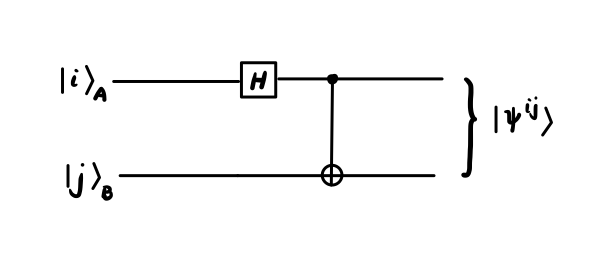
\includegraphics[scale = 1]{bell.png}
\end{center}
The Bell states are often used as a basis resource in quantum information protocols (quantum teleportation, quantum key distribution, entanglement enhanced ``abc'' - protocols).
\subsubsection{Distinction between Entangled States and Mixed States}
A bipartite state $\rho_{AB} \in \rho(\hilbert_A \otimes \hilbert_B)$ is called:
\begin{quote}
    1. a product state, if $\rho_{AB} = \rho_A \otimes \rho_B$, and $\rho_A \in \mathcal{S}(\hilbert_A), \rho_B \in \mathcal{S}(\hilbert_B)$. \\
    2. a \impt{separable} state, if $\displaystyle \rho_{AB} = \Sumi{k} q_k \rho_A^{(k)} \otimes \rho_B^{(k)}$.
    $$\rho_{AB} = \frac{1}{5} \dyad{+}\otimes\dyad{0} + \frac{4}{5}\dyad{0}\otimes\dyad{-}$$
    3. an entangled state, if $\rho_{AB}$ is not separable.
\end{quote}
\begin{definition}
    \uimpt{Werner states} are states $\rho_{AB} = \lambda \dyad{\psi^{01}} + (1-\lambda)\frac{\id_4}{4}$, where $\lambda \in [0,1]$. It can be shown that Werner states are entangled when $\lambda > \frac{2}{3}$.
\end{definition}

\subsection{Quantum Teleportation - 量子遥传}
The setting of quantum teleportation is the following:
\begin{quote}
    1. Two agents (Alice and Bob) are placed in different locations. \\
    2. They share a maximally entangled state, say $\ket{\psi^{00}}_{AB}$. \\
    3. They can exchange classical bits. \\
    4. Alice holds a qubit $S$, where $\ketpsi_S = \alpha\ket{0}_S + \beta\ket{1}_S$.
\end{quote}
The goal is to ``teleport'' $\ketpsi_S$ to Bob's system, or preparing $\ketpsi_B$ on $B$ by only exchanging classical information.
\begin{center}
    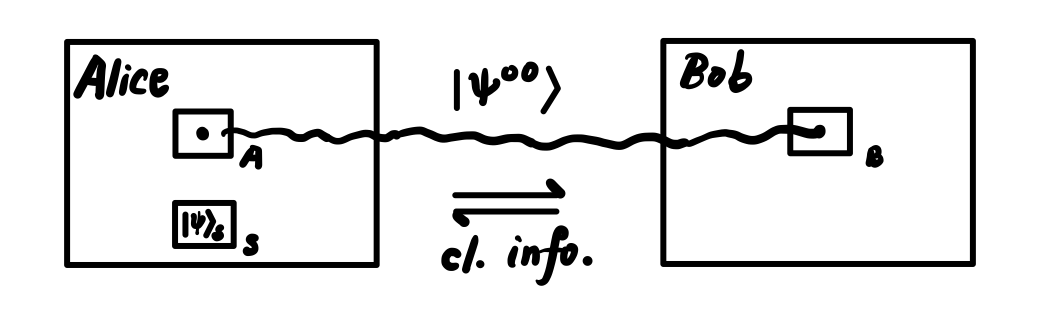
\includegraphics[scale = 0.8]{qtele-setup.png}
\end{center}
The protocol is as follows:
\begin{center}
    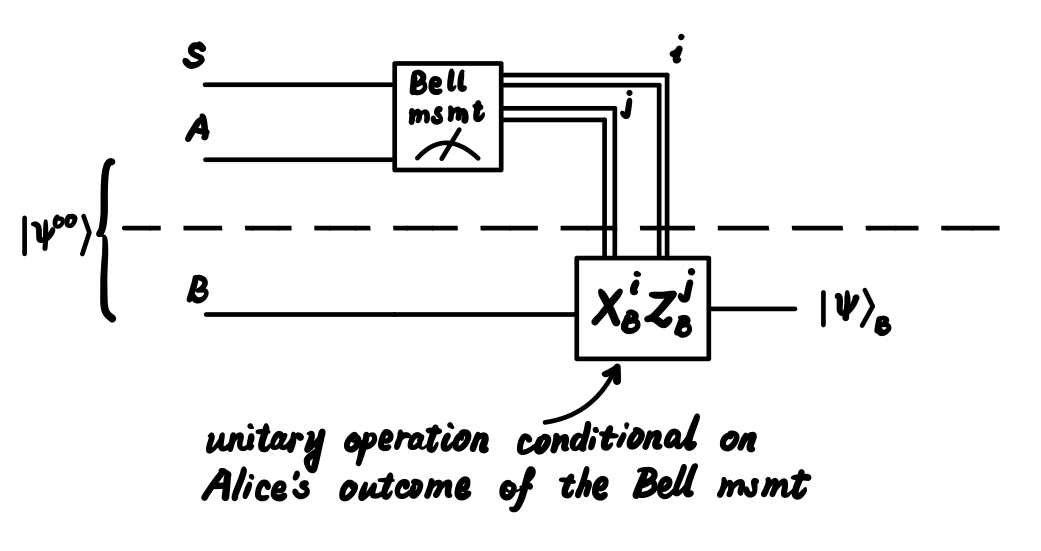
\includegraphics[scale = 0.8]{qtele-protocol.png}
\end{center}
where the Bell measurement is inversed in this case:
\begin{center}
    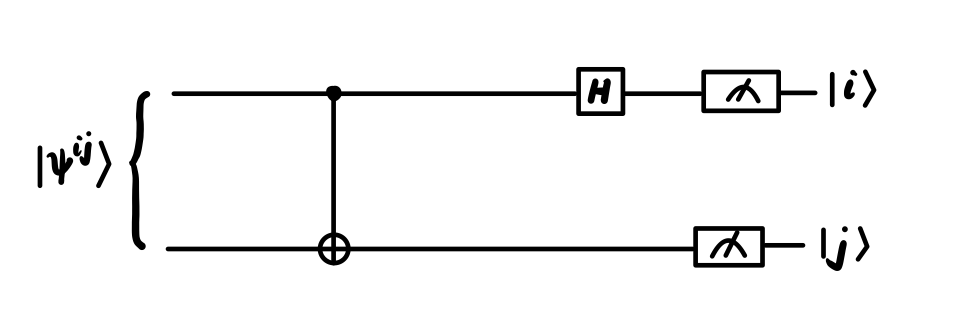
\includegraphics[scale = 0.8]{bell-inverse.png}
\end{center}
We now analyze this circuit. Suppose the initial state to be:
\begin{align*}
    \ketPsi_{SAB} &= \ketpsi_S \otimes \ket{\psi^{00}}_{AB} \\
    &= (\alpha \ket{0} + \beta \ket{1})_S \otimes \frac{1}{\sqrt{2}}(\ket{00}_{AB} + \ket{11}_{AB}) \\
    &= \frac{\alpha}{2}\ket{000} + \frac{\alpha}{011} + \frac{\beta}{2}\ket{100} + \frac{\beta}{2}\ket{111}
\end{align*}
Further suppose the outcome from the inverse Bell measurement $i = 1, j = 0$ is obtained, then the post-measurement state on $SAB$ is:
\begin{align*}
    \ket{\Psi_{(1, 0)}'}_{SAB} &= \frac{1}{\text{norm.}}(\dyad{\psi^{10}}\otimes \id_B)\ketPsi_{SAB} \\
    &= \ket{\psi^{10}} \otimes (\alpha \ket{1} + \beta\ket{0})
\end{align*}
Bob now applies $X_B^1Z_B^0 = X_B$, the final state on $B$ will be:
$$X_B(\alpha \ket{1} + \beta\ket{0}) = \alpha \ket{0} + \beta\ket{1}$$
Note that, quantum teleportation works independently of $\alpha, \beta \in \C$, hence it also works these values are unknown. The transmission of $2$ classical bits is necessary and optimal, without knowing $(i, j)$, Bob's state is maximally mixed. The classical analogue is rather straightforward, that is transmitting a classical bit from $A$ to $B$. Without knowing the bit initially, we simply look at the bit to know the value and sent it across. This is not useful for qubits because a measurement on $S$ alone does not allow us to know $\alpha, \beta$.


\subsection{No-cloning Theorem - 不可克隆原理}
The na\"ive idea for ``quantum teleportation'' is to copy $\ketpsi$ many times, and measure the copies to obtain good estimates for $\alpha, \beta$, then send these values as classical information for Bob to prepare. However, this does not work. 
\begin{definition}
    Consider two quantum systems $\hilbert_A \cong \hilbert_B$, a \uimpt{quantum cloning operation} on $\hilbert_A$ is a process that achieves:
    $$\forall \ketpsi_A \in \hilbert_A, \ketpsi_A\ket{0}_B \mapsto \ketpsi_A\ketpsi_B$$
\end{definition}
Note that CNOT is not a cloning operation because:
$$\ketplus_A \ket{0}_B \mapsto \ket{\psi^{00}} \ne \ketplus_A\ketplus_B$$
\begin{theorem}
    The \uimpt{no-cloning theorem} states that it is impossible to clone an unknown quantum state.
\end{theorem}
The proof for this theorem is as follows: \\
A cloning process would have to achieve
\begin{center}
    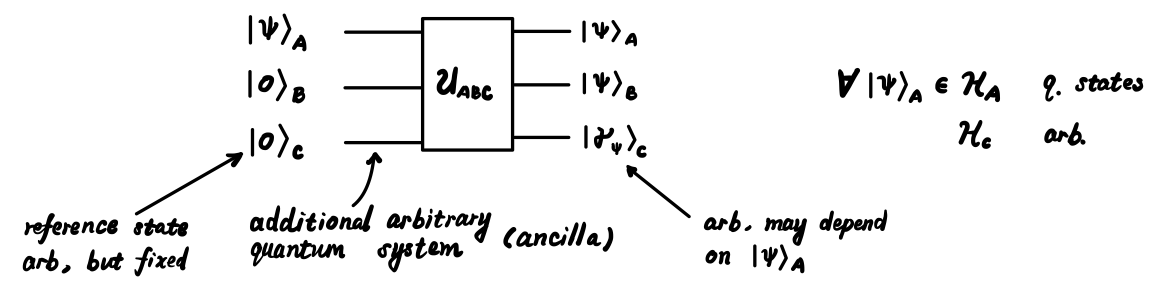
\includegraphics[scale = 0.75]{clone.png}
\end{center}
Consider another state $\ketphi_A \in \hilbert_A$ where $0 < \abs{\braket{\psi}{\psi}} < 1$. Recall that unitary operators should \impt{preserve inner products}, then we have:
\begin{align*}
    \abs{\braket{\psi 0 0}{\phi 0 0}} &= \abs{\braket{\psi}{\phi}_A} \\
    \abs{\braket{\psi\psi\gamma_\psi}{\phi \phi \gamma_\phi}} &= \abs{\braket{\psi}{\phi}_A} \cdot \abs{\braket{\psi}{\phi}_B} \cdot \abs{\braket{\gamma_\psi}{\gamma_\phi}_C} \\
    &\le \abs{\braket{\psi}{\phi}_A}^2
\end{align*}
However, $\abs{\braket{\psi}{\phi}_A} > \abs{\braket{\psi}{\phi}_A}^2$, by it being between $0$ and $1$, we see that it contradicts with the unitary preserving inner products. \\
Note that the evolutions in nature are all unitary evolutions, it is crucial to see that they are linear operations. And the key reason why cloning is impossible is that it is not a linear operation. \\
The no-cloning theorem thus implies that there is no na\"ive quantum teleportation; there is no na\"ive quantum error correction protocol; it is the basis of security proofs for quantum cryptography (quantum key distribution); and it implies monogamy of non-classical correlations. \\
Specifically, for error correction protocol, this prevents us from doing:
$$\ketpsi = \alpha \ket{0} + \beta \ket{1} \mapsto (\alpha \ket{0} + \beta \ket{1})^{\otimes n}$$
and we do this instead:
$$\alpha \ket{0} + \beta \ket{1} \mapsto \alpha\ket{000} + \beta\ket{111}$$
\begin{center}
    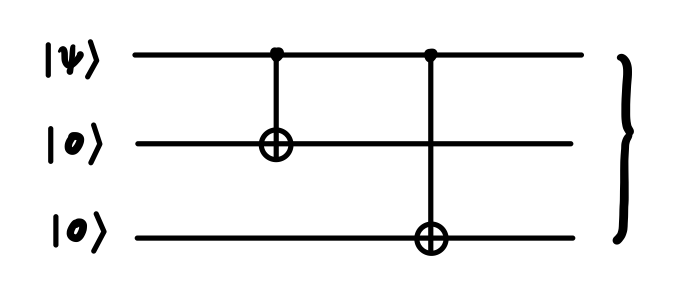
\includegraphics[scale = 1]{error-correction.png}
\end{center}
Furthermore, specifically for quantum cryptography, consider the situation where there exists an ``Eve'' who wishes to know the key between Alice and Bob, then:
\begin{center}
    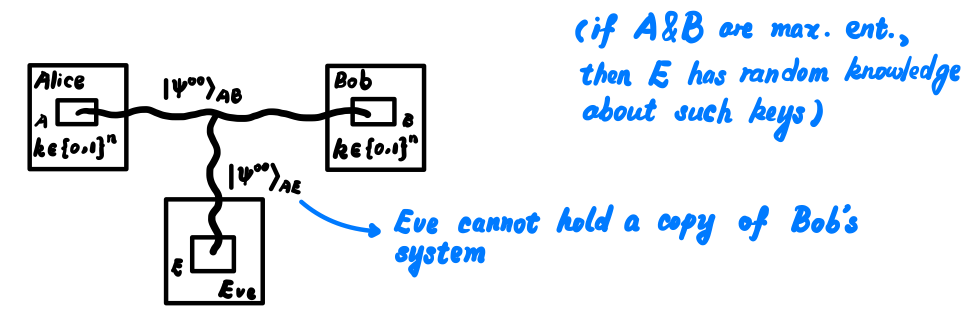
\includegraphics[scale = 0.75]{quantum-security.png}
\end{center}
Eve is being prevented from knowing the key because if Eve forms such entangled states, she would have an exact copy of Bob's system. Only Eve or Bob (one person) can be maximally entangled with Alice, but not both.
\begin{definition}
    \uimpt{Monogamy of non-classical correlations} means if two parties are correlated to the maximal extent possible, then they cannot be correlated with any other system in the world.
\end{definition}
\bigskip
\begin{center}
    {\huge \textbf{Marchons, marchons !}}
\end{center}

\end{document}